%
%  PARA TRABALLOS EN GALLEGO USAR (LINEA 12): \usepackage[galician]{babel}
%  PARA TRABALLOS EN CASTELLANO USAR (LINEA 13): \usepackage[spanish]{babel}
%
% Para los acentos usamos codificacion UTF-8 (LINEA 10): \usepackage[utf8]{inputenc} 
% Si se usase la codificacion es_ES.ISO-8859-1 (LINEA 11): \usepackage[latin1]{inputenc}
% La conversion de acentos se hace con: iconv -f UTF-8 -t ISO-8859-1 filename.tex
%
% Como se incluyen figuras eps hay que compilar con: latex traballo , dvipdf traballo
%

\documentclass[12pt,twoside,a4paper]{book}
% pódense engadir todos os packages necesarios
\usepackage[utf8]{inputenc}
% \usepackage[latin1]{inputenc}
% \usepackage[galician]{babel}
\usepackage[spanish,es-tabla]{babel}
\usepackage{graphicx}
\usepackage{grffile}
\usepackage[dvips]{epsfig}
\usepackage{amssymb}
\usepackage{enumitem}
\usepackage{eurosym}
\usepackage{float}
\usepackage{latexsym}
\usepackage{a4}
\usepackage{listings}
\usepackage{hyperref} % menús no pdf pero non leva ben co package galician
\usepackage{supertabular}
\usepackage{hhline}
\usepackage{amsmath}
\usepackage{amssymb,amsfonts,textcomp}
\usepackage{array}
\usepackage{longtable} 
\usepackage{tabularx}
\usepackage{multirow}
\usepackage{titlesec}
\usepackage{pdflscape}
\usepackage{listings}


\usepackage{color}
\definecolor{lightgray}{rgb}{.9,.9,.9}
\definecolor{darkgray}{rgb}{.4,.4,.4}
\definecolor{purple}{rgb}{0.65, 0.12, 0.82}
\lstdefinelanguage{JavaScript}{
  keywords={break, case, catch, continue, debugger, default, delete, do, else, false, finally, for, function, if, in, instanceof, new, null, return, switch, this, throw, true, try, typeof, var, void, while, with},
  morecomment=[l]{//},
  morecomment=[s]{/*}{*/},
  morestring=[b]',
  morestring=[b]",
  ndkeywords={class, export, boolean, throw, implements, import, this},
  keywordstyle=\color{blue}\bfseries,
  ndkeywordstyle=\color{darkgray}\bfseries,
  identifierstyle=\color{black},
  commentstyle=\color{purple}\ttfamily,
  stringstyle=\color{red}\ttfamily,
  sensitive=true
}

\lstset{
   language=JavaScript,
   backgroundcolor=\color{lightgray},
   extendedchars=true,
   basicstyle=\footnotesize\ttfamily,
   showstringspaces=false,
   showspaces=false,
   numbers=left,
   numberstyle=\footnotesize,
   numbersep=9pt,
   tabsize=2,
   breaklines=true,
   showtabs=false,
   captionpos=b
}


\begin{document}

%\pagestyle{empty}
\begin{center}
{\bf\Large UNIVERSIDADE DE SANTIAGO DE COMPOSTELA}

\vspace{0.5cm}

\includegraphics[width=5cm]{figuras/logo_usc.eps}

\vspace{0.5cm}
{\bf\large ESCOLA TÉCNICA SUPERIOR DE ENXEÑARÍA}

\vspace{2cm}
{\bf\LARGE Título do Traballo de Fin de Grao}

\vspace{0.5cm}
{\bf\LARGE Subtítulo do Traballo de Fin de Grao}
\end{center}

\vspace{2cm}
\hspace{4cm}\begin{tabular}{l}
{\it\Large Autor:} \\
{\bf\Large Nome do autor} \\
~ \\
{\it\Large Directores:} \\
{\bf\Large Nome do director} \\
{\bf\Large Nome do codirector} \\
\end{tabular}

\vspace{2cm}
\begin{center}
{\bf\Large Grao en Enxeñaría Informática}

\vspace{0.5cm}
{\bf\large Febreiro 2011}

\vspace{0.5cm}
Traballo de Fin de Grao presentado na Escola Técnica Superior de Enxeñaría da Universidade de Santiago de Compostela para a obtención do Grao en Enxeñaría Informática
\end{center}


%\cleardoublepage
%\pagestyle{plain}
\pagenumbering{roman}

\includegraphics[width=4cm]{figuras/logo_usc.eps}

\vspace{1cm}
{\bf D. José Manuel Cotos Yáñez}, Profesor del Departamento de Electrónica y Computación de la Universidad de Santiago de Compostela,
% e {\bf D. (Nome do Codirector)}, Profesor do Departamento de Electrónica e Computación da Universidade de Santiago de Compostela,

\vspace{1cm}
%INFORMAN:
INFORMA:

\vspace{1cm}
Que la presente memoria, titulada {\it Emozio}, presentada por {\bf D.ª Raquel Gil Martínez} para superar los créditos correspondientes al Trabajo de Fin de Grado de la titulación de Grado en Ingeniería Informática, se realizó bajo nuestra dirección en el Departamento de Electrónica y Computación de la Universidad de Santiago de Compostela.

\vspace{1cm}
Y para que así conste a los efectos oportunos, expide el presente informe en Santiago de Compostela, a 5 de febrero de 2018:

\vspace{2cm}
\begin{tabular}{lll}
%O director, & O codirector, & O alumno, \\
El director, & El alumno, \\
~ \\
~ \\
~ \\
~ \\
~ \\
~ \\
~ \\
%(Nome do director) & (Nome do Codirector) & (Nome do Alumno)
José Manuel Cotos Yáñez & Raquel Gil Martínez
\end{tabular}

 % paxina de certificación (optativa)
%\cleardoublepage
%\pagestyle{plain}
\chapter*{Agradecementos}
Se se quere pór algún agradecemento, este vai aquí.

 % paxina de agradecementos (optativa) 
%\cleardoublepage
%\pagestyle{plain}
\chapter*{Resumo}
Se se quere pór resumo, este vai aquí.

 % páxina de resumo (optativa) 

\cleardoublepage
\pagestyle{plain}
\tableofcontents
\listoffigures
\listoftables

% Agora incluimos os capítulos. Cambiamos a numeración e as cabeceiras
\cleardoublepage
\pagenumbering{arabic}
\setcounter{page}{1}
\pagestyle{headings}
%\chapter{Introdución}

El curso pasado (2016-2017) participé en el programa para emprendedores Yuzz “Jóvenes con ideas”, donde aprendí a convertir una idea empresarial en un modelo de negocio. 


Mi equipo promotor estaba compuesto por Bruno Rodríguez, psicólogo, y yo misma. Nuestra vocación hacia la aportación de soluciones en el campo de la salud mental, se vio impulsada por la adecuada combinación entre nuestras experiencias y estudios, dando lugar a nuestro proyecto empresarial Emozio. 


\section{Contexto}
Emozio será una plataforma web de búsqueda de psicólogos, donde el paciente cubre un test validado científicamente que permitirá a la plataforma asignar al profesional más adecuado para tratar su problema. Se trata pues de una plataforma de servicios de emparejamiento entre un paciente y el mejor profesional disponible. 


La finalidad es ofrecer el mejor especialista para solucionar el problema que tiene un determinado usuario, solventando la tediosa y difícil tarea de encontrar un psicólogo competente cuando surge la necesidad, y evitando terapias inefectivas. 


Por otro lado, la mayoría de los psicólogos que ejercen su profesión tienen la necesidad de encontrar un flujo constante de pacientes para mantener a flote su consulta/despacho, por lo que pertenecer a nuestro catálogo supondrá un plús añadido a sus servicios ya que éstos serán respaldados por un sello de calidad (Emozio) que hará posible el aumento y fidelización de clientes/pacientes. Así como, aportarles visualización y publicidad con costes más reducidos que los existentes.


\section{Objetivos}
El objetivo del proyecto es desarrollar una plataforma web que permita la búsqueda de psicólogos, donde, por un lado, los pacientes cubren un test que permitirá caracterizarlos, de forma que la plataforma pueda asignarles el profesional más adecuado para tratar su problema. Por otro lado, la plataforma ha de permitir a los psicólogos darse de alta como profesionales caracterizados por su \textit{expertise}. Dicha plataforma, ha de estar provista de diferentes servicios comunes como la gestión los usuarios (pacientes y psicólogos), posibilitar el filtrado de los psicólogos que aparecen como resultado del test en función de diferentes parámetros y poner en contacto el paciente con el psicólogo en cuestión... 


Se pretende que la plataforma desarrollada en el marco de trabajo del TFG, sirva como producto mínimo viable (PMV) del modelo de negocio, por lo que se persigue poder mostrar el producto como un prototipo a los usuarios finales. 


En concreto, se persigue conseguir los siguientes objetivos transversales:


\begin{itemize}
\item Desarrollar una plataforma web.
\item Permitir que los pacientes cubran un test que los pueda caracterizar.
\item Emparejar a los pacientes con los psicólogos que puedan tratarles.
\item Realizar la gestión de usuarios.
\item Permitir el filtrado en los resultados del test.
\item Permitir la comunicación entre pacientes y psicólogos.
\end{itemize}


\section{Estructura de la memoria}

%\cleardoublepage
%GESTIÓN DEL PROYECTO
%\chapter{Gestión del proyecto}

%%%%%%%%%%%%%%%%%%%%%%%%%%%%%%%%%%%%%%%%%%%%%%%%%%%%%%%%%%%%%%%%%%%%%%%%%%%%%%%%%%%%%
%%%%%%%%%%%%%%%%%%%%%%%%%%%%%%%%%%%%%%%%%%%%%%%%%%%%%%%%%%%%%%%%%%%%%%%%%%%%%%%%%%%%%
%%%%%%%%%%%%%%%%%%%%%%%%%%%%%%%%%%%%%%%%%%%%%%%%%%%%%%%%%%%%%%%%%%%%%%%%%%%%%%%%%%%%%

\section{Alcance del proyecto}

Según el PMBOK \cite{pmbok} se trata del trabajo realizado para entregar un producto, servicio o resultado con las funciones y características especificadas. La línea base del proyecto, consistirá en el eunciado del alcance, la estructura de desglose de trabajo (EDT/WBS) y el diccionario EDT/WBS asociado.

\subsection{Enunciado del alcance}
La joven startup Emozio necesita una plataforma web para llevar a cabo su modelo de negocio, el cual consiste en la asignación del psicólogo más adecuado para tratar la patología de un paciente. 
Como se trata de una startup que ha surgido de forma reciente, todavía precisan validar y afianzar su propuesta de valor para lanzarla al mercado. Por tanto, su requisito primordial es disponer de un producto mínimo viable que les permita mostrar su propuesta a su público objetivo.


Para desempeñar la característica principal del producto, se precisará de un cuestionario que evalúe los síntomas del paciente, caracterizando así la posible patología que este presenta. Una vez realizado el cuestionario, la plataforma dará como resultado del mismo a un listado de psicólogos que podrían tratar esa patología. Además, éste resultado podrá ser filtrado por distintos campos, como el precio, el seguro de salud, si se trata de una cita presencial u online, entre otros. 


A su vez, debe permitir al paciente ponerse en contacto con el psicólogo del listado por el que desea ser atendido. Este mensaje de contacto, podrá visualizarlo el psicólogo a través de su bandeja de entrada. 


Cabe decir, que tanto psicólogos como pacientes podrán darse de alta en la plataforma y hacer uso de sus servicios, por lo que se necesitará una mínima gestión de usuarios. 


Para que el paciente pueda evaluar la cita recibida por el psicólogo, éste podrá dejar un comentario con una valoración en su perfil para que pueda ser compartido al resto de usuarios. De esta forma, se dará la transparencia necesaria al servicio de recomendación lo que nos valdrá de sello de calidad.

\subsection{Criterios de aceptación}
Las condiciones que deben cumplirse para que el proyecto sea aceptado son:

\begin{itemize}
\item Entrega en plazo de todos los entregables.
\item Realización de los requisitos establecidos.
\end{itemize}

\subsection{Entregables del proyecto}
Se deberá hacer entrega de:

\begin{itemize}
\item Tres copias en papel de la memoria
\item Una copia en soporte digital de:
	\begin{itemize}
		\item La memoria
		\item El código fuente
		\item El ejecutable
	\end{itemize}
\end{itemize}

\subsection{Exclusiones del proyecto}
Las exclusiones aplicadas al proyecto son:

\begin{itemize}
\item El mantenimiento y soporte de la plataforma una vez realizada la entrega.
\item Análisis de campo e investigación asociada al desarrollo del cuestionario científico de asignación.
\end{itemize}

\subsection{Restricciones del proyecto}
El alcance de este proyecto sólo abarcará a lo que se corresponde con el producto mínimo viable de lo que será la plataforma real de Emozio, y que servirá como punto de partida para la implementación de la misma. Su pretensión no se trata de realizar el desarrollo completo de la aplicación con todas sus características totalmente funcionales, sino realizar una primera aproximación a la misma.

\subsection{Supuestos del proyecto}
Asumimos que al tratarse de un producto mínimo viable, no se podrá estimar el crecimiento del sistema tanto a nivel de funcionalidades como en el contenido de la base de datos, por lo que no se podrá preveer cómo será la escalabilidad real del sistema.

\subsection{Estructura de descomposición de tareas (EDT/WBS) del proyecto}
La estructura de descomposición de tareas viene representada en la figura \ref{fig:edt}.

\begin{figure}[htbp] 
    \centering
    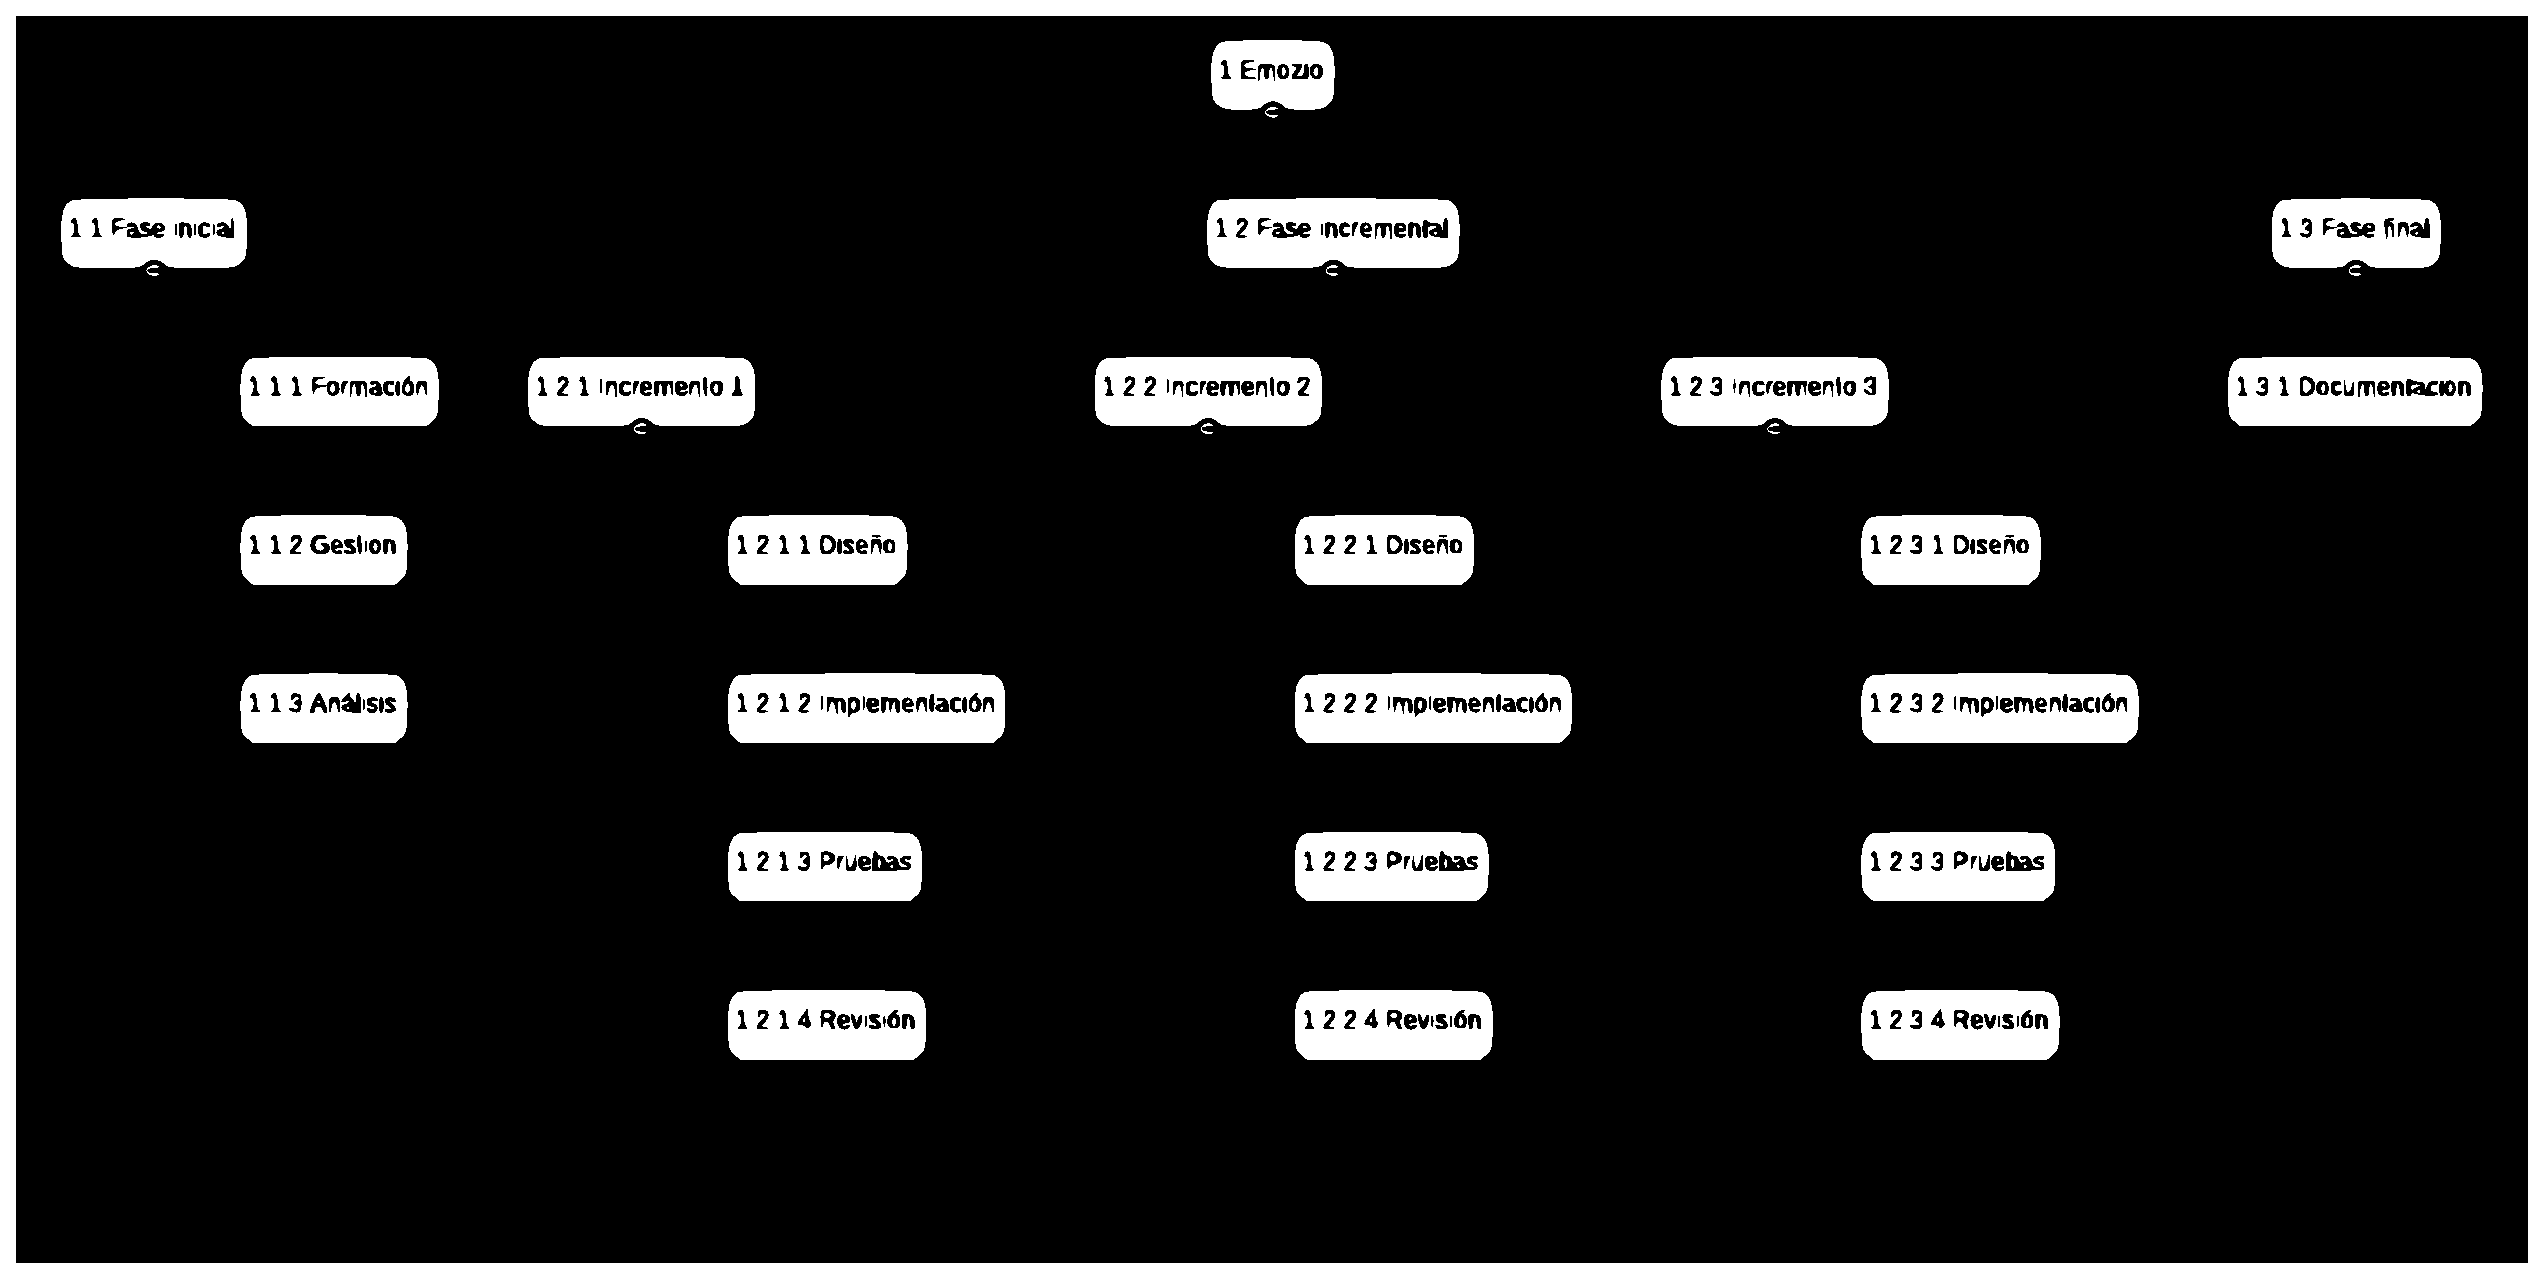
\includegraphics[width=1\textwidth]{figuras/edt.eps}
    \caption{Estructura de descomposición de tareas del proyecto}
    \label{fig:edt}
\end{figure}	

\subsubsection{Diccionario EDT/WBS}
El proyecto está dividido en tres fases: Inicial, incremental y final. Éstas se encuentran descritas en mayor detalle en la sección donde se detalla la metodología de desarrollo utilizada.

\begin{itemize}[label={}]
\item \textbf{Fase inicial}
Compuesta por la formación en las principales tecnologías utilizadas (\textit{Stack MEAN framework}), la elaboración de la gestión del proyecto y un primer ánalisis inicial del producto.
\item \textbf{Fase incremental}
Se encuentra dividida entre los tres incrementos que se van a realizar, cada uno con sus respectivas tareas: Diseño, implementación, pruebas y revisión.
\item \textbf{Fase final}
En ella se elaborará toda la documentación final del proyecto que se va a presentar: La memoria, el manual de instalación y el manual de usuario.
\end{itemize} 

%%%%%%%%%%%%%%%%%%%%%%%%%%%%%%%%%%%%%%%%%%%%%%%%%%%%%%%%%%%%%%%%%%%%%%%%%%%%%%%%%%%%%
%%%%%%%%%%%%%%%%%%%%%%%%%%%%%%%%%%%%%%%%%%%%%%%%%%%%%%%%%%%%%%%%%%%%%%%%%%%%%%%%%%%%%
%%%%%%%%%%%%%%%%%%%%%%%%%%%%%%%%%%%%%%%%%%%%%%%%%%%%%%%%%%%%%%%%%%%%%%%%%%%%%%%%%%%%%

\section{Metogología de desarrollo}
Una metodología de desarrollo de software en ingeniería de software es un marco de trabajo usado para estructurar, planificar y controlar el proceso de desarrollo en sistemas de información.


Según Pressman\cite{pressman}, cualquier proceso del software ágil se caracteriza por la forma en la que aborda cierto número de suposiciones clave acerca de la mayoría de proyectos de software:

\begin{itemize}
\item Es difícil predecir que requerimientos de software persistirán y cuales cambiarán o pronosticar como cambiaron las prioridades del cliente a medida que avanza el proyecto.
\item En muchos tipos de software el diseño y la construcción de ejecutarse en forma simultánea de modo que los modelos de diseño se prueban a medida que se crean.
\item El análisis , el diseño, la construcción y las pruebas no son tan predecibles como nos gustaría.
\end{itemize} 


Las principales motivaciones para utilizar este tipo de metología se trataban de:

\begin{itemize}
\item Inicialmente, se desconocía tanto el algoritmo que se iba a utilizar para el emparejamiento, así como la caracterización de los pacientes y psicólogos; y la información que era necesario almacenar en la base datos.
\item No tenía total disponibilidad de mi \textit{stakeholder} el cuál me iba a proporcionar el \textit{feedback} e información necesaria del sistema.
\item Por otra parte, sí se tenían claro los subsistemas que se requerían dentro de la plataforma.
\item Como se trata de un proyecto que surge de un estado del arte, necesitábamos gran margen para introducir cambios y poder integrarlos.
\item La inexperiencia en las tecnologías utilizadas podrían suponer que hubiese continuos cambios en el diseño y el código de la plataforma.
\end{itemize}


Por tanto, se requería un proceso adaptativo e incremental, donde en cada incremento se desarrollase uno de los subsistemas identificados en nuestra plataforma.


En este tipo de procesos, deben entregarse incrementos de software (prototipos ejecutables o porciones de un sistema) en periodos cortos de tiempo. Este enfoque iterativo permite que el cliente evalúe de forma regular el incremento de software, dé la retroalimentación necesaria e influya en las adaptaciones del proceso que se realicen para aprovechar esa retroalimentación.


Las fases que se van a realizar en este proyecto son:
\begin{enumerate}
\item \textbf{Fase Inicial:} Conlleva la gestión de proyecto, la formación y un primer análisis inicial de lo que sería la plataforma.
\item \textbf{Fase incremental:} En esta fase se realizarán los tres incrementos.
\item \textbf{Fase final:} Se realizará la documentación del proyecto.
\end{enumerate}

\subsubsection{Fase incremental}
En esta sección se describirán con mayor detalle en qué consisten los tres incrementos del proceso. Donde cada uno de ellos tendrá sus propias fases de diseño, implementación, pruebas y revisión.

\textbf{Incremento 1}


El primer incremento se realizará justo después de la fase inicial, y se corresponde con el subsistema del cuestionario de emparejamiento paciente-psicólogo.


Según la planificación temporal descrita en la gestión de tiempos, se prevé que el incremento 1 comience el día 9 de noviembre y finalice el 6 de diciembre. Esta previsión tiene en cuenta que es el primer contacto directo con las tecnologías utilizadas por lo que es predecible que se trabaje de forma más pautada y se produzcan muchos ensayo-error. Además de que en él se implementa la complejidad algorítmica relacionada con el emparejamiento.


\textbf{Incremento 2}


Tras finalizar el primer incremento, se procede a realizar este segundo que se corresponde con el subsistema de gestión de usuarios.


Según la planificación prevista, estará comprendido entre el 7 de diciembre y el 20 de diciembre.


\textbf{Incremento 3}


El último incremento es el qué involucra al subsistema de comunicación. 


Siguiendo la planificación temporal realizada, durará desde el 21 de diciembre hasta el 3 de enero.


A lo largo de esta memoria cada tarea realizada, estará definida dentro del contexto del incremento en el cual se realiza.

%%%%%%%%%%%%%%%%%%%%%%%%%%%%%%%%%%%%%%%%%%%%%%%%%%%%%%%%%%%%%%%%%%%%%%%%%%%%%%%%%%%%%
%%%%%%%%%%%%%%%%%%%%%%%%%%%%%%%%%%%%%%%%%%%%%%%%%%%%%%%%%%%%%%%%%%%%%%%%%%%%%%%%%%%%%
%%%%%%%%%%%%%%%%%%%%%%%%%%%%%%%%%%%%%%%%%%%%%%%%%%%%%%%%%%%%%%%%%%%%%%%%%%%%%%%%%%%%%

\section{Planificación temporal}
La previsión temporal del presente proyecto estaba comprendido entre el 16 de octubre de 2017 y el 21 de enero de 2018, con un trabajo de seis horas diarias. La estimación temporal en tareas, y la asignación de las mismas a los recursos, se puede observar en el diagrama de Gantt \ref{fig:gantt}.

\begin{figure}[htbp] 
    \centering
    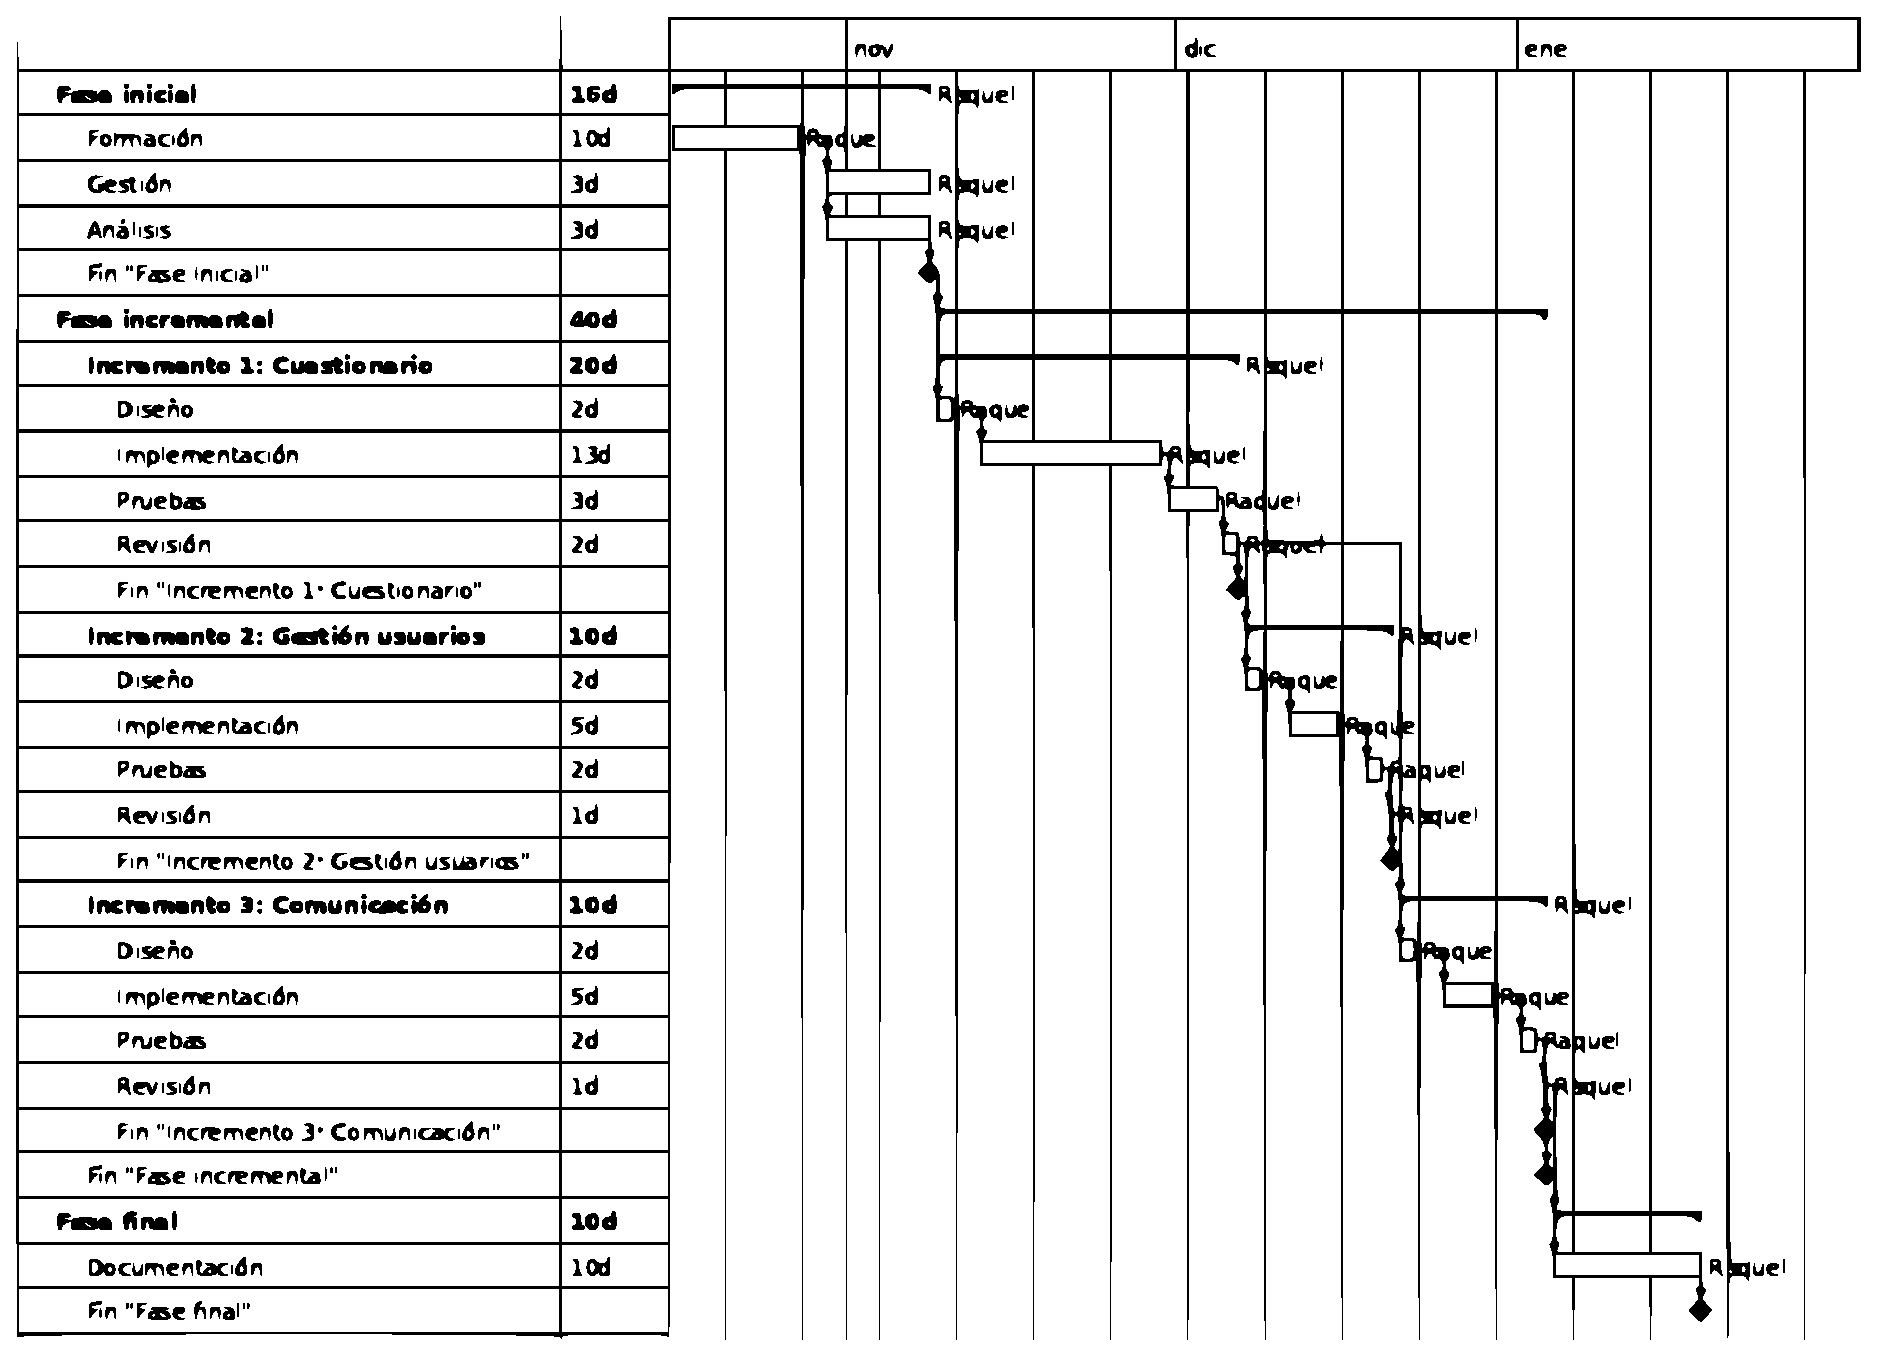
\includegraphics[width=1\textwidth]{figuras/gantt.eps}
    \caption{Diagrama de Gantt}
    \label{fig:gantt}
\end{figure}	

%%%%%%%%%%%%%%%%%%%%%%%%%%%%%%%%%%%%%%%%%%%%%%%%%%%%%%%%%%%%%%%%%%%%%%%%%%%%%%%%%%%%%
%%%%%%%%%%%%%%%%%%%%%%%%%%%%%%%%%%%%%%%%%%%%%%%%%%%%%%%%%%%%%%%%%%%%%%%%%%%%%%%%%%%%%
%%%%%%%%%%%%%%%%%%%%%%%%%%%%%%%%%%%%%%%%%%%%%%%%%%%%%%%%%%%%%%%%%%%%%%%%%%%%%%%%%%%%%

\section{Gestión de la configuración}
La gestión de la configuración del software es un conjunto de actividades diseñadas para administrar el cambio mediante la identificación de los productos de trabajo con potencial de cambio, las relacines entre ellos, la definición de mecanismos para administrar diferentes versiones de los mismos y el control de los cambios impuestos, así como la auditoría y reporte de los cambios realizados\cite{pressman}.

\subsection{Línea base}
El IEEE (IEEE Std. No. 610.12-1990) indica que una especificación o producto que se revisó formalmente y con el que se estuvo de acuerdo, servirá como base para un mayor desarrollo y que cambia sólo a través de procedimientos de control de cambio formal.


Las líneas base de nuestro proyecto son fundamentalmente el enunciado del alcance del proyecto y los requisitos software.

\subsubsection{Creación de líneas base}
Como nuestro proyecto se desarrolla de manera incremental, la línea base del segundo incremento, será tanto el enunciado del alcance del proyecto, los requisitos software asociados a dicho incremento y finalmente, el código resultado del incremento 1. De forma análoga sería para el caso del incremento 3, que tendría como línea base adicional el código resultado del incremento 2.

\subsection{Repositorio para la gestión de la configuración}
Un repositorio es el conjunto de mecanismos y estructuras de datos que permiten administrar el cambio de forma efectiva, asegurando la integridad, posibilidad de compartir e integrar datos. Para lograr estas capacidades, el repositorio se define como un metamodelo que determina cómo se almacena la información en el repositorio, cómo pueden acceder las herramientas a los datos, cuán bien puede mantenerse la seguridad e integridad de los datos y cuán fácilmente puede extenderse el modelo existente para alojar nuevas necesidades\cite{pressman}.

\subsubsection{Repositorio escogido}
Este proyecto se encuentra almacenado en un repositorio GitHub que es una plataforma de desarrollo colaborativo de software para alojar proyectos usando el sistema de control de versiones Git\cite{github}. Git nos permitirá tener una copia del repositorio del proyecto en local y otra en remoto. El proyecto en local sufrirá constantes modificaciones, que una vez validadas, se guardarán en el remoto.

\subsubsection{Metamodelo}
La estructura de información que se encuentra en el repositorio viene definida en la figura \ref{tab_metamodelo}.

\begin{table}[htpb]
\centering
\caption{Metamodelo}
\label{tab_metamodelo}
\begin{tabularx}{\textwidth}{|l|l|X|}
\hline
\multicolumn{2}{|c|}{Carpeta}                     & \multicolumn{1}{c|}{Descripción del contenido}                                                                             \\ \hline
\multicolumn{2}{|X|}{em\_diagramas}               & Contiene el archivo de StarUML que contiene todos los diagramas del proyecto: Casos de uso, modelo de datos, patrón MVC... \\ \hline
\multirow{7}{*}{em\_memoria} & em\_analisis       & Contiene todos los archivos referentes al análisis.                                                                        \\ \cline{2-3} 
                             & em\_anexos         & Contiene todos los anexos de la memoria del proyecto.                                                                      \\ \cline{2-3} 
                             & em\_diseño         & Contiene todos los archivos referentes al diseño.                                                                          \\ \cline{2-3} 
                             & em\_gest\_proy     & Contiene todos los archivos referentes a la gestión del proyecto.                                                          \\ \cline{2-3} 
                             & em\_introducción   & Contiene la introducción de la memoria del proyecto.                                                                       \\ \cline{2-3} 
                             & em\_memoria\_final & Se trata del documento en LaTeX que contiene la memoria a entregar.                                                        \\ \cline{2-3} 
                             & em\_plan\_pruebas  & Contiene todos los archivos referentes al plan de pruebas.                                                                 \\ \hline
\multicolumn{2}{|X|}{em\_mockup}                  & Contiene el mockup hecho con Pencil de la plataforma web.                                                                  \\ \hline
\multicolumn{2}{|X|}{em\_web}                     & Contiene todos los archivos que constituyen el código fuente de la plataforma web.                                         \\ \hline
\end{tabularx}
\end{table}

Dentro de cada carpeta o subcarpeta, los archivos aparecen con un nombre descriptivo. Por ejemplo, en la subcarpeta de \texttt{em\_memoria} llamada \texttt{em\_gest\_proy} se encuentra \texttt{gest\_costes.odt} que es el archivo correspondiente a la subsección de costes de la sección de gestión del proyecto que habrá en la memoria final.

\subsection{Sistema de gestión de la configuración}
La estructura del repositorio está distribuida del siguiente modo:

\begin{enumerate}
\item \textbf{Master}
Contendrá la última versión validada del código fuente, es decir, tras pasar las pruebas del incremento 1, contendrá el código fuente del incremento 1, y así, sucesivamente.
\item \textbf{Branches}
	\begin{itemize}
	\item \textbf{memoria\_branch}
	Contendrá los commits de las distintas versiones de la memoria del proyecto.
	\item \textbf{diagrama\_branch}
	Contendrá los commits de las distintas versiones de los diagramas de la plataforma.
	\item \textbf{mockup\_branch}
	Contendrá los commits de las distintas versiones del mockup de la plataforma.
	\item \textbf{cuestionario\_branch, usuarios\_branch y contacto\_branch}
	Contendrán respectivamente, los commits del código fuente asociado a los incrementos 1, 2 y 3.
	Antes de comenzar un incremento, se crea una branch de master y se implementan las funcionalidades pertenecientes a ese incremento. Una vez realizada su fase de pruebas, se hará un merge de esa branch con el master, y posteriormente, se elimina.
	\end{itemize}
\end{enumerate}


%%%%%%%%%%%%%%%%%%%%%%%%%%%%%%%%%%%%%%%%%%%%%%%%%%%%%%%%%%%%%%%%%%%%%%%%%%%%%%%%%%%%%
%%%%%%%%%%%%%%%%%%%%%%%%%%%%%%%%%%%%%%%%%%%%%%%%%%%%%%%%%%%%%%%%%%%%%%%%%%%%%%%%%%%%%
%%%%%%%%%%%%%%%%%%%%%%%%%%%%%%%%%%%%%%%%%%%%%%%%%%%%%%%%%%%%%%%%%%%%%%%%%%%%%%%%%%%%%

\section{Gestión de costes}

%%%%%%%%%%%%%%%%%%%%%%%%%%%%%%%%%%%%%%%%%%%%%%%%%%%%%%%%%%%%%%%%%%%%%%%%%%%%%%%%%%%%%
%%%%%%%%%%%%%%%%%%%%%%%%%%%%%%%%%%%%%%%%%%%%%%%%%%%%%%%%%%%%%%%%%%%%%%%%%%%%%%%%%%%%%
%%%%%%%%%%%%%%%%%%%%%%%%%%%%%%%%%%%%%%%%%%%%%%%%%%%%%%%%%%%%%%%%%%%%%%%%%%%%%%%%%%%%%

\section{Gestión de riesgos}

\subsection{Plan de gestión de riesgos}
El riesgo de un proyecto es un evento o condición incierta que, de producirse, tiene un efecto positivo o negativo en uno o más de los objetivos del proyecto. Éste, puede tener una o más causas, y de materializarse, uno o más impactos\cite{pmbok}.


Para poder preveer estas consecuencias, se debe llevar un registro de los posibles riesgos que pueden acontecer. Así, una vez identificados y analizados, podemos planificar las respuestas para los mismos.


Para poder definir la probabilidad e impacto de la materialización de un riesgo, se deben definir las escalas correspondientes a los mismos. Para poder medir la probabilidad e impacto que puede tener un riesgo se han creado las tablas \ref{tab_probabilidad} y \ref{tab_impacto}.


La \textbf{probabilidad} representa la expectativa de ocurrencia real del riesgo, y el \textbf{impacto}, representa el efecto que la ocurrencia del riesgo tendría en el desarrollo del proyecto, en términos de coste, esfuerzo o duración total del mismo. 

\begin{table}[htpb]
\centering
\caption{Valoración del impacto}
\label{tab_impacto}
\begin{tabular}{|l|l|}
\hline
\multicolumn{2}{|c|}{Valoración del impacto}                                                  \\ \hline
\multicolumn{1}{|c|}{Repercusión en Plazo / Esfuerzo / Costes} & \multicolumn{1}{c|}{Impacto} \\ \hline
\textgreater= 20\%                                             & Alto                         \\ \hline
Entre 10\% y 20 \%                                             & Medio                        \\ \hline
\textless= 10\%                                                & Bajo                         \\ \hline
\end{tabular}
\end{table}

\begin{table}[htpb]
\centering
\caption{Valoración de la probabilidad}
\label{tab_probabilidad}
\begin{tabular}{|l|l|}
\hline
\multicolumn{2}{|c|}{Valoración de la probabilidad} \\ \hline
\multicolumn{1}{|c|}{Ocurrencia del Riesgo}             & \multicolumn{1}{c|}{Probabilidad}  \\ \hline
\textgreater= 80\% (casi segura)  & Alta          \\ \hline
Entre 30\% y 80\% (muy probable)  & Media         \\ \hline
\textless= 30\% (poco probable)   & Baja         \\ \hline
\end{tabular}
\end{table}

Si vinculamos la probabilidad de ocurrencia de cada riesgo con su impacto sobre los objetivos del proyecto en caso de que ocurra dicho riesgo, podemos obtener la matriz que representa el nivel de exposición al riesgo (dado por el producto del impacto por la probabilidad). Esta matriz \ref{tab_riesgo} determinará la gestión de los riesgos del proyecto.

\begin{table}[htpb]
\centering
\caption{Nivel de exposición al riesgo}
\label{tab_riesgo}
\begin{tabular}{|l|l|l|l|l|}
\hline
\multicolumn{5}{|c|}{Nivel de exposición al riesgo}                         \\ \hline
\multicolumn{2}{|l|}{\multirow{2}{*}{}} & \multicolumn{3}{c|}{Probabilidad} \\ \cline{3-5} 
\multicolumn{2}{|l|}{}                  & Alta      & Media     & Baja      \\ \hline
\multirow{3}{*}{Impacto}     & Alto     & Alto      & Alto      & Medio     \\ \cline{2-5} 
                             & Medio    & Alto      & Medio     & Bajo      \\ \cline{2-5} 
                             & Bajo     & Medio     & Bajo      & Bajo      \\ \hline
\end{tabular}
\end{table}

\subsection{Identificación de riesgos}
Tras identificar los riesgos por medio  de revisión de la documentación, tormenta de ideas y análisis de supuestos, se procede a la elaboración del siguiente registro de riesgos \ref{tab_reg_riesgos}.

\begin{table}[htpb]
\centering
\caption{Registro de riesgos}
\label{tab_reg_riesgos}
\begin{tabularx}{\textwidth}{|l|X|X|}
\hline
\multicolumn{1}{|c|}{Identificador} & \multicolumn{1}{c|}{Nombre}                        & \multicolumn{1}{c|}{Descripción}                                                                                                                                                              \\ \hline
RSG-001                             & Práctica deficiente de la gestión de proyectos     & Se produce una práctica deficiente en la gestión de proyectos debido a la inexperiencia.                                                                                                      \\ \hline
RSG-002                             & Dependencia de participantes externos              & Existe dependencia de participantes externos fuera del ámbito de control directo del proyecto como el tutor que guía el proyecto o el experto psicólogo.                                      \\ \hline
RSG-003                             & Falta de experiencia en las tecnologías utilizadas & La inexperiencia en las tecnologías utilizadas puede repercutir en la planificación prevista del proyecto.                                                                                    \\ \hline
RSG-004                             & Pérdida de información                             & Se puede producir la pérdida de información debido a un mal guardado de los datos en el respositorio.                                                                                         \\ \hline
RSG-005                             & Retraso en la planificación temporal               & Acontece un retraso en la planificación temporal prevista debido a causas externas como enfermedad o asuntos personales.                                                                      \\ \hline
RSG-006                             & Caída de la red proveedora de Internet             & Una caída de la red proveedora de Internet puede causar retrasos en la planificación o pérdida deinformación.                                                                                 \\ \hline
RSG-007                             & Fallo de suministro eléctrico                      & Un fallo del suministro eléctrico  puede causar retrasos en la planificación o pérdida deinformación.                                                                                         \\ \hline
RSG-008                             & Ataques maliciosos en el equipo de trabajo         & Un ataque malicioso en el equipo de trabajo puede significar que existe una brecha de seguridad en el sistema por lo que existe un posible robado de datos o incluso pérdidas de información. \\ \hline
\end{tabularx}
\end{table}

\subsection{Análisis cualitativo de riesgos}
Mediante el análisis cualitativo de los riesgos podemos evaluar la prioridad de los riesgos identificados a través de la probabilidad relativa de ocurrencia, del impacto correspondiente sobre los objetivos del proyecto si los riesgos llegasen a presentarse. Esta evaluación \ref{tab_eval_riesgos} refleja la actitud que existe frente a los riesgos. 

\begin{table}[htpb]
\centering
\caption{Evaluación de los riesgos}
\label{tab_eval_riesgos}
\begin{tabularx}{\textwidth}{|l|X|l|l|l|}
\hline
\multicolumn{1}{|c|}{Identificador} & \multicolumn{1}{c|}{Nombre}                        & \multicolumn{1}{c|}{Probabilidad} & \multicolumn{1}{c|}{Impacto} & \multicolumn{1}{c|}{Exposición} \\ \hline
RSG-001                             & Práctica deficiente de la gestión de proyectos     & Media                             & Alto                         & Alto                            \\ \hline
RSG-002                             & Dependencia de participantes externos              & Alta                              & Medio                        & Alto                            \\ \hline
RSG-003                             & Falta de experiencia en las tecnologías utilizadas & Alta                              & Alto                         & Alto                            \\ \hline
RSG-004                             & Pérdida de información                             & Baja                              & Alto                         & Medio                           \\ \hline
RSG-005                             & Retraso en la planificación temporal               & Baja                              & Medio                        & Bajo                            \\ \hline
RSG-006                             & Caída de la red proveedora de Internet             & Baja                              & Alto                         & Medio                           \\ \hline
RSG-007                             & Fallo de suministro eléctrico                      & Baja                              & Alto                         & Medio                           \\ \hline
RSG-008                             & Ataques maliciosos en el equipo de trabajo         & Baja                              & Alto                         & Medio                           \\ \hline
\end{tabularx}
\end{table}

La matriz de exposición de los riesgos \ref{tab_mat_exp_riesgo} da a conocer las prioridades de acción en el caso de que se materializasen los riesgos.

\begin{table}[htpb]
\centering
\caption{Matriz de exposición de los riesgos}
\label{tab_mat_exp_riesgo}
\begin{tabular}{|c|c|l|l|l|}
\hline
\multicolumn{2}{|l|}{\multirow{2}{*}{}} & \multicolumn{3}{c|}{Probabilidad}                                                                                                      \\ \cline{3-5} 
\multicolumn{2}{|l|}{}                  & \multicolumn{1}{c|}{Alta} & \multicolumn{1}{c|}{Media} & \multicolumn{1}{c|}{Baja}                                                     \\ \hline
\multirow{3}{*}{Impacto}     & Alto     & RSG-003                   & RSG-001                    & \begin{tabular}[c]{@{}l@{}}RSG-004\\ RSG-006\\ RSG-007\\ RSG-008\end{tabular} \\ \cline{2-5} 
                             & Medio    & RSG-002                   &                            & RSG-005                                                                       \\ \cline{2-5} 
                             & Bajo     &                           &                            &                                                                               \\ \hline
\end{tabular}
\end{table}

\subsection{Plan de respuesta a los riesgos}
Con la planificación de respuesta a los riesgos se busca desarrollar opciones y acciones para mejorar las oportunidades y reducir las amenazas a los objetivos del proyecto. Las respuestas a los riesgos deben adecuarse a laimportancia del riesgo, ser rentables con relación al desafía a cumplir,  realistas dentro del contexto del proyecto y a cargo de una persona responsable \cite{pmbok}.


Debido a que sólo existe una persona a cargo del proyecto, ésta será la responsable de acatar las medidas oportunas.


\begin{table}[htpb]
\centering
\caption{Plan de respuesta RSG-001}
%\label{my-label}
\begin{tabularx}{\textwidth}{|l|X|}
\hline
RSG-001              & Práctica deficiente de la gestión de proyectos                                                                      \\ \hline
Acción de prevención & Mitigar. Se asegurará que la persona encargada de la gestión de proyectos se forme específicamente en dicho ámbito. \\ \hline
Indicador            & La persona encargada de la gestión no efectúa adecuadamente los procesos a seguir.                                  \\ \hline
Acción de corrección & Se dedicarán más horas de trabajo a la gestión de proyectos.                                                        \\ \hline
\end{tabularx}
\end{table}


\begin{table}[htpb]
\centering
\caption{Plan de respuesta RSG-002}
%\label{my-label}
\begin{tabularx}{\textwidth}{|l|X|}
\hline
RSG-002              & Dependencia de participantes externos                                                                                                                                                                  \\ \hline
Acción de prevención & Aceptar. Debido a la imprevisión que supone estar a expensas de otro stakeholder del proyecto se acepta la posible aparición del riesgo y se trata de continuar con el normal desarrollo del proyecto. \\ \hline
Indicador            & Ausencia o falta de respuesta por parte de un stakeholder.                                                                                                                                             \\ \hline
Acción de correccion & Se procederá a abordar las distintas tareas de forma ficticia o en último recurso se obviarán.                                                                                                        \\ \hline
\end{tabularx}
\end{table}


\begin{table}[htpb]
\centering
\caption{Plan de respuesta RSG-003}
%\label{my-label}
\begin{tabularx}{\textwidth}{|l|X|}
\hline
RSG-003              & Falta de experiencia en las tecnologías utilizadas                                                                \\ \hline
Acción de prevención & Mitigar. Se formará al trabajador en las tecnologías utilizadas antes de comenzar con el desarrollo del proyecto. \\ \hline
Indicador            & El trabajador desconoce cómo implementar determinada funcionalidad                                                \\ \hline
Acción de correccion & Se pausará por un determinado tiempo el desarrollo y se estudiará lo necesario para poder continuar.              \\ \hline
\end{tabularx}
\end{table}


\begin{table}[htpb]
\centering
\caption{Plan de respuesta RSG-004}
%\label{my-label}
\begin{tabularx}{\textwidth}{|l|X|}
\hline
RSG-004              & Pérdida de información                                                                                                  \\ \hline
Acción de prevención & Evitar. Se harán volcados del trabajo realizado en el respositorio de forma periódica de al menos dos días de trabajo.  \\ \hline
Indicador            & Los últimos cambios efectuados no están reflejados en los archivos de trabajo ni en la última versión del respositorio. \\ \hline
Acción de corrección & Se repartirá el número de horas de trabajo correspondiente a esa parte durante el próximo periodo de la planificación.  \\ \hline
\end{tabularx}
\end{table}


\begin{table}[htpb]
\centering
\caption{Plan de respuesta RSG-005}
%\label{my-label}
\begin{tabularx}{\textwidth}{|l|X|}
\hline
RSG-005              & Retraso en la planificación temporal                                                                                                                                                     \\ \hline
Acción de prevención & Aceptar. Debido a que se puede producir un retraso en la planificación temporal por causas ajenas al proyecto, se aceptará este hecho y se tratará de continuar con la mayor normalidad. \\ \hline
Indicador            & Surge una enfermedad o un asunto personal.                                                                                                                                               \\ \hline
Acción de corrección & Se reubicará la carga de trabajo prevista y que no haya sido realizada a lo largo del periodo que vaya a continuación.                                                                   \\ \hline
\end{tabularx}
\end{table}


\begin{table}[htpb]
\centering
\caption{Plan de respuesta RSG-006}
%\label{my-label}
\begin{tabularx}{\textwidth}{|l|X|}
\hline
RSG-006              & Caída de la red proveedora de Internet                                                                                                                                                                 \\ \hline
Acción de prevención & Mitigar. Se dispondrá de una red alternativa a la que usamos de forma habitual.                                                                                                                        \\ \hline
Indicador            & Falla la conexión a Internet o no se encuentra la red.                                                                                                                                                 \\ \hline
Acción de corrección & Se procederá a buscar una red alternativa. Por ejemplo, en el caso de estar trabajando con la conexión WiFi y que ésta sufra una caída, proceder a conectarnos a la red móvil del \textit{smartphone} personal. \\ \hline
\end{tabularx}
\end{table}


\begin{table}[htpb]
\centering
\caption{Plan de respuesta RSG-007}
%\label{my-label}
\begin{tabularx}{\textwidth}{|l|X|}
\hline
RSG-007              & Fallo de suministro eléctrico                                                                                                                                 \\ \hline
Acción de prevención & Aceptar. Si el fallo de suministro eléctrico causa una pérdida del trabajo realizado, se asumen las consecuencias y se procede a partir de la última versión. \\ \hline
Indicador            & El ordenador se queda sin suministro eléctrico de forma repentina tras una subida de tensión.                                                                 \\ \hline
Acción de corrección & Se rehará el trabajo a partir de la última versión guardada.                                                                                                  \\ \hline
\end{tabularx}
\end{table}


\begin{table}[htpb]
\centering
\caption{Plan de respuesta RSG-008}
%\label{my-label}
\begin{tabularx}{\textwidth}{|X|l|}
\hline
RSG-008              & Ataques maliciosos en el equipo de trabajo                                                                                                                                                              \\ \hline
Acción de prevención & Evitar. No descargar recursos de fuentes no fiables, no utilizar el ordenador de trabajo como ordenador personal, no dejar la sesión abierta en caso de ausencia y que ésta posea contraseña de acceso. \\ \hline
Indicador            & Fallos desconocidos hasta el momento en el sistema, pérdida de información, comportamiento sospechosos del funcionamiento del ordenador...                                                              \\ \hline
Acción de corrección & Se hará un formateo del sistema y se recuperarán los últimos cambios, de ser afectados, de la última versión del repositorio.                                                                           \\ \hline
\end{tabularx}
\end{table}







%\cleardoublepage
%ANÁLISIS
%\section{Análisis}

La ingeniería de requisitos proporciona el mecanismo apropiado para entender lo que dice el cliente, analizar las necesidades, evaluar la factibilidad, negociar una solución, especificar la solución sin ambigüedades, validar la especificación y administrar los requisitos a medida que se transforman en un sistema funcional\cite{pressman}.

\subsection{Casos de uso}
Para poder entender cómo los usuarios emplearán finalmente las funciones y características del software, se debe crear un conjunto de escenarios que identifiquen la naturaleza de los usos para el sistema que se va a construir. La descripción de la manera en la que se utilizará el sistema se la conoce como caso de uso.

\subsubsection{Actores del sistema}
Un actor\ref{tab_actores} es cualquier cosa que se comunica con el sistema o producto y que sea externo a este. 

\begin{table}[htpb]
\centering
\begin{tabularx}{\textwidth}{|l|X|X|}
\hline
\multicolumn{1}{|c|}{Identificador} & \multicolumn{1}{c|}{Nombre} & \multicolumn{1}{c|}{Descripción}                                 \\ \hline
ACT-001                             & Usuario                     & Cualquier persona que acceda a nuestra plataforma web.           \\ \hline
ACT-002                             & Paciente                    & Cualquier persona que desee ser evaluada por nuestra aplicación. \\ \hline
ACT-003                             & Psicólogo                   & Cualquier persona que ejerza profesionalmente como psicólogo.    \\ \hline
ACT-004                             & Sistema                     & Encargado de ejecutar el algoritmo de emparejamiento.            \\ \hline
ACT-005                             & Administrador               & Persona encargada de gestionar los recursos de la aplicación.    \\ \hline
\end{tabularx}
\caption{Actores del sistema}
\label{tab_actores}
\end{table}


\subsubsection{Especificación de casos de uso}
Para poder determinar y evaluar corréctamente cada caso de uso, tenemos una escala de la frecuencia de uso\ref{tab_frec_uso} y otra de la prioridad\ref{tab_prior}.

\begin{table}[htpb]
\centering
\begin{tabularx}{\textwidth}{|l|X|}
\hline
\multicolumn{2}{|c|}{Frecuencia de uso}                                                   \\ \hline
Ocasionalmente & Se utilizará en algunas ocasiones, no de forma habitual o por costumbre. \\ \hline
Puntualmente   & Se utilizará en raras ocasiones.                                         \\ \hline
Limitada       & Sólo podrá utilizarse en una única ocasión.                              \\ \hline
\end{tabularx}
\caption{Frecuencias de uso}
\label{tab_frec_uso}
\end{table}

\begin{table}[htpb]
\centering
\begin{tabularx}{\textwidth}{|l|X|}
\hline
\multicolumn{2}{|c|}{Prioridad}                                                                          \\ \hline
Alta  & El caso de uso es imprescindible para el funcionamiento normal de la aplicación.                 \\ \hline
Media & El caso de uso aporta funcionalidad necesaria en el sistema pero no aporta un valor fundamental. \\ \hline
Baja  & El caso de uso aporta funcionalidades extra pero es totalmente prescindible.                     \\ \hline
\end{tabularx}
\caption{Prioridades}
\label{tab_prior}
\end{table}

%
%CU-001
%
%
\begin{table}[htpb]
\centering
\begin{tabularx}{\textwidth}{|l|X|}
\hline
CU-001                            & Iniciar sesión                                                                                                                                                                                                                                   \\ \hline
Actor principal                   & Usuario                                                                                                                                                                                                                                          \\ \hline
Objetivo en contexto              & El actor desea acceder a una cuenta de usuario ya existente mediante sus claves de acceso.                                                                                                                                                       \\ \hline
Precondiciones                    & Las claves de usuario deben ser válidas.                                                                                                                                                                                                         \\ \hline
Disparador                        & El actor desea acceder a la plataforma para disfrutar de sus servicios.                                                                                                                                                                          \\ \hline
Escenario                         & \begin{tabular}{p{0.5cm} p{6cm}}1. & El actor accede a Emozio.\\ 2. & El actor introduce sus clavesde acceso.\\ 3. & El actor pulsa el botón de acceso.\\ 4. & El sistema muestra el perfil del actor donde podrá acceder al resto de servicios.\end{tabular} \\ \hline
Excepciones                       & \begin{tabular}{p{0.5cm} p{6cm}}1. & Las claves de usuario son incorrectas.\\ 2. & El actor no estaba registrado en la plataforma en el momento que se realizó el acceso.\end{tabular}                                                                    \\ \hline
Prioridad                         & Alta. El actor debe iniciar sesión en la aplicación para poder utilizar cualquiera de sus servicios.                                                                                                                                             \\ \hline
Disponibilidad                    & En el segundo incremento                                                                                                                                                                                                                         \\ \hline
Frecuencia de uso                 & Ocasionalmente                                                                                                                                                                                                                                   \\ \hline
Canal del actor                   & A través de un navegador con acceso a internet.                                                                                                                                                                                                  \\ \hline
Dependencias (con los requisitos) & \begin{tabular}[c]{@{}l@{}}RI-001\\ RI-003\\ RF-001\end{tabular}                                                                                                                                                                                 \\ \hline
\end{tabularx}
\caption{CU-001 Iniciar sesión}
%\label{my-label}
\end{table}

%%
%%CU-002
%%

\begin{table}[htpb]
\centering
\begin{tabularx}{\textwidth}{|l|X|}
\hline
CU-002                            & Registrarse                                                                                                                                                                                                                                                                                                                                                                                                                    \\ \hline
Actor principal                   & Usuario                                                                                                                                                                                                                                                                                                                                                                                                                        \\ \hline
Objetivo en contexto              & El actor desea registrarse en la plataforma cediendo sus datos personales para poder acceder a los servicios de la plataforma.                                                                                                                                                                                                                                                                                                 \\ \hline
Precondiciones                    & Los datos introducidos en el formulario deben ser válidos.                                                                                                                                                                                                                                                                                                                                                                     \\ \hline
Disparador                        & El actor desea registrarse en la plataforma para disfrutar de sus servicios.                                                                                                                                                                                                                                                                                                                                                   \\ \hline
Escenario                         & \begin{tabular}{p{0.5cm} p{6cm}} 1. & El actor accede a Emozio. \\ 2. & El actor introduce sus datos en un formulario de registro.\\ 3. & El actor pulsa el botón de registro.\\ 4. & Se completa el registro.\\ 4.1. & Si es paciente, el sistema muestra el perfil del usuario donde podrá acceder al resto de servicios.\\ 4.2. & Si es psicólogo, sus datos son enviados por correo para que el administrador pueda validarlos.\end{tabular} \\ \hline
Excepciones                       & \begin{tabular}{p{0.5cm} p{6cm}}1. & Los datos introducidos en el formulario son incorrectos.\\ 2. & Ya existe el usuario dentro de la plataforma.\end{tabular}                                                                                                                                                                                                                                                                         \\ \hline
Prioridad                         & Alta. El actor debe estar registrado en la aplicación para poder utilizar cualquiera de sus servicios.                                                                                                                                                                                                                                                                                                                         \\ \hline
Disponibilidad                    & En el segundo incremento                                                                                                                                                                                                                                                                                                                                                                                                       \\ \hline
Frecuencia de uso                 & Limitada                                                                                                                                                                                                                                                                                                                                                                                                                       \\ \hline
Canal del actor                   & A través de un navegador con acceso a internet.                                                                                                                                                                                                                                                                                                                                                                                \\ \hline
Dependencias (con los requisitos) & \begin{tabular}[c]{@{}l@{}}RI-001\\ RI-003\\ RF-001\\ RF-002\end{tabular}                                                                                                                                                                                                                                                                                                                                                      \\ \hline
\end{tabularx}
\caption{CU-002 Registrarse}
%\label{my-label}
\end{table}

%%
%%CU-003
%%

\begin{table}[htpb]
\centering
\begin{tabularx}{\textwidth}{|X|X|}
\hline
CU-003                            & Realizar cuestionario                                                                                                                                                                                                                                                                                                                                                                                                                                                                                                    \\ \hline
Actor principal                   & Paciente                                                                                                                                                                                                                                                                                                                                                                                                                                                                                                                 \\ \hline
Objetivo en contexto              & El paciente desea conocer qué profesional es el más adecuado para tratar su dolencia realizando el cuestionario de emparejamiento.                                                                                                                                                                                                                                                                                                                                                                                       \\ \hline
Precondiciones                    & El cuestionario debe estar cubierto.                                                                                                                                                                                                                                                                                                                                                                                                                                                                                     \\ \hline
Disparador                        & El paciente debe haber pulsado el botón de “hacer el cuestionario”.                                                                                                                                                                                                                                                                                                                                                                                                                                                      \\ \hline
Escenario                         & \begin{tabular} {p{0.5cm} p{5cm}} 1. & El  paciente accede a Emozio.\\ 2. & El paciente entra en su perfil de usuario ya sea por registro o acceso.\\  3. & El sistema le muestra su perfil de usuario.\\ 4. & El paciente pulsa el botón de hacer el cuestionario.\\ 5. & El sistema le muestra el formulario que debe cubrir.\\ 6. & El paciente cubre las respuestas del formulario.\\ 7. & El paciente pulsa el botón de conocerlos resultados.\\ 8. & El sistema le mostrará su perfil en el que se encuentran los resultados.\end{tabular} \\ \hline
Excepciones                       & Los datos introducidos en el formulario son incorrectos.                                                                                                                                                                                                                                                                                                                                                                                                                                                                 \\ \hline
Prioridad                         & Alta. Es la característica central de la plataforma.                                                                                                                                                                                                                                                                                                                                                                                                                                                                     \\ \hline
Disponibilidad                    & En el primer incremento                                                                                                                                                                                                                                                                                                                                                                                                                                                                                                  \\ \hline
Frecuencia de uso                 & Puntualmente                                                                                                                                                                                                                                                                                                                                                                                                                                                                                                             \\ \hline
Canal del actor                   & A través de un navegador con acceso a internet.                                                                                                                                                                                                                                                                                                                                                                                                                                                                          \\ \hline
Dependencias (con los requisitos) & \begin{tabular}[c]{@{}l@{}}RI-001\\ RI-002\\ RI-003\\ RF-001\\ RF-002\\  RF-005\end{tabular}                                                                                                                                                                                                                                                                                                                                                                                                                                       \\ \hline
\end{tabularx}
\caption{CU-003 Realizar cuestionario}
%\label{my-label}
\end{table}

%%
%%CU-004
%%

\begin{table}[htpb]
\centering
\begin{tabularx}{\textwidth}{|X|X|}
\hline
CU-004                            & Consultar resultados                                                                                                                                                                                                                                                     \\ \hline
Actor principal                   & Paciente                                                                                                                                                                                                                                                                 \\ \hline
Objetivo en contexto              & El paciente desea consultar el resultado del cuestionario de asignación.                                                                                                                                                                                                 \\ \hline
Precondiciones                    & El cuestionario debe estar cubierto.                                                                                                                                                                                                                                     \\ \hline
Disparador                        & El paciente debe acceder a su perfil.                                                                                                                                                                                                                                    \\ \hline
Escenario                         & \begin{tabular}{p{0.5cm} p{5cm}} 1. & El paciente accede a Emozio. \\ 2. & El paciente entra en su perfil de usuario ya sea por registro o acceso.\\ 3. & El sistema le muestra su perfil de usuario donde se encuentran los resultados del cuestionario de asignación.\end{tabular} \\ \hline
Excepciones                       & El paciente no ha cubierto el test en ninguna ocasión.                                                                                                                                                                                                                   \\ \hline
Prioridad                         & Alta. Es la característica central de la plataforma.                                                                                                                                                                                                                     \\ \hline
Disponibilidad                    & En el primer incremento                                                                                                                                                                                                                                                  \\ \hline
Frecuencia de uso                 & Ocasionalmente                                                                                                                                                                                                                                                           \\ \hline
Canal del actor                   & A través de un navegador con acceso a internet.                                                                                                                                                                                                                          \\ \hline
Dependencias (con los requisitos) & \begin{tabular}[c]{@{}l@{}}RI-001\\ RI-003\\ RF-001\\ RF-002\\ RF-005\\ RF-006\end{tabular}                                                                                                                                                                                       \\ \hline
\end{tabularx}
\caption{CU-004 Consultar resultados}
%\label{my-label}
\end{table}

%%
%%CU-005
%%

\begin{table}[htpb]
\centering
\begin{tabularx}{\textwidth}{|X|X|}
\hline
CU-005                            & Contactar psicólogo                                                                                                                                                                                                                                                                                                                                                                                                                                                                                                                                                                                                                                                                                                        \\ \hline
Actor principal                   & Paciente                                                                                                                                                                                                                                                                                                                                                                                                                                                                                                                                                                                                                                                                                                                   \\ \hline
Objetivo en contexto              & El paciente desea ponerse en contacto con uno de los psicólogos que le han sido asignados.                                                                                                                                                                                                                                                                                                                                                                                                                                                                                                                                                                                                                                 \\ \hline
Precondiciones                    & \begin{tabular}{p{0.5cm} p{5cm}}1.  &  El cuestionario debe estar cubierto.\\ 2.  &  Las respuestas del cuestionario no dieron resultados imprecisos.\end{tabular}                                                                                                                                                                                                                                                                                                                                                                                                                                                                                                                                \\ \hline
Disparador                        & El paciente  accede a su perfil y se decide a contactar con el psicólogo.                                                                                                                                                                                                                                                                                                                                                                                                                                                                                                                                                                                                                                                  \\ \hline
Escenario                         & \begin{tabular}{p{0.5cm} p{5cm}}1.  &  El  paciente accede a Emozio.\\ 2.  &  El paciente entra en su perfil de usuario ya sea por registro o acceso.\\ 3.  &  El sistema le muestra su perfil de usuario donde se encuentran los resultados del cuestionario de asignación.\\ 4.  &  El paciente pulsa el botón de contacto del psicólogo en cuestión.\\ 5.  &  El sistema le muestra un formulario de contacto que debe cubrir.\\ 6.  &  El paciente cubre el formulario.\\ 7.  &  El paciente pulsa el botón de enviar.\\ 8.  &  El sistema muestra un mensaje con el estado de la operación.\end{tabular} \\ \hline
Excepciones                       & \begin{tabular}{p{0.5cm} p{5cm}}1.  &  El paciente no ha cubierto el test en ninguna ocasión.\\ 2.  &  El test dió un resultado impreciso para las respuestas dadas en el cuestionario.\end{tabular}                                                                                                                                                                                                                                                                                                                                                                                                                                                                                              \\ \hline
\end{tabularx}
\caption{CU-005 Contactar psicólogo - Parte 1}                                                                                                                                                                                                                                                                                                                                                                                                                                                                                                                                                                                                                                                                                                 
%\label{my-label}
\end{table}

\begin{table}[htpb]
\centering
\begin{tabularx}{\textwidth}{|X|X|}
\hline
CU-005                            & Contactar psicólogo                                                                                                                                                                                                                                                                                                                                                                                                                                                                                                                                                                                                                                                                                                        \\ \hline
Prioridad                         & Moderada. Puede implementarse después de las funciones básicas.                                                                                                                                                                                                                                                                                                                                                                                                                                                                                                                                                                                                                                                            \\ \hline
Disponibilidad                    & En el tercer incremento                                                                                                                                                                                                                                                                                                                                                                                                                                                                                                                                                                                                                                                                                                    \\ \hline
Frecuencia de uso                 & Puntualmente                                                                                                                                                                                                                                                                                                                                                                                                                                                                                                                                                                                                                                                                                                               \\ \hline
Canal del actor                   & A través de un navegador con acceso a internet.                                                                                                                                                                                                                                                                                                                                                                                                                                                                                                                                                                                                                                                                            \\ \hline
Dependencias (con los requisitos) & \begin{tabular}[c]{@{}l@{}}RI-001\\ RI-003\\ RF-001\\ RF-002\\ RF-005\end{tabular}                                                                                                                                                                                                                                                                                                                                                                                                                                                                                                                                                                                             \\ \hline
\end{tabularx}
\caption{CU-005 Contactar psicólogo - Parte 2}                                                                                                                                                                                                                                                                                                                                                                                                                                                                                                                                                                                                                                                                                                 
%\label{my-label}
\end{table}

%%
%%CU-006
%%

\begin{table}[htpb]
\centering
\begin{tabularx}{\textwidth}{|X|X|}
\hline
CU-006                            & Modificar información                                                                                                                                                                                                                                                                                                                                                                                                                                                                                \\ \hline
Actor principal                   & Usuario                                                                                                                                                                                                                                                                                                                                                                                                                                                                                              \\ \hline
Objetivo en contexto              & El usuario desea cambiar sus datos porque en ese instante su información de usuario es incorrecta.                                                                                                                                                                                                                                                                                                                                                                                                   \\ \hline
Precondiciones                    & El usuario tiene acceso a la plataforma.                                                                                                                                                                                                                                                                                                                                                                                                                                                             \\ \hline
Disparador                        & El usuario debe acceder a su página principal.                                                                                                                                                                                                                                                                                                                                                                                                                                                       \\ \hline
Escenario                         & \begin{tabular}{p{0.5cm} p{5cm}}1. & El usuario accede a Emozio.\\ 2. & El usuario entra en su página principal ya sea por registro o acceso.\\ 3. & El sistema le muestra su página principal.\\ 4. & El usuario pulsa el botón de modificación de datos.\\ 5. & El sistema le muestra un formulario con sus datos actuales.\\ 6. & El usuario cubre el formulario con los datos correctos.\\ 7. & El usuario pulsa el botón de enviar.\\ 8. & El sistema muestra un mensaje con el estado de la operación.\end{tabular} \\ \hline
Excepciones                       & El usuario cancela la operación en curso.                                                                                                                                                                                                                                                                                                                                                                                                                                                            \\ \hline
Prioridad                         & Moderada. Puede implementarse después de las funciones básicas.                                                                                                                                                                                                                                                                                                                                                                                                                                      \\ \hline
Disponibilidad                    & En el segundo incremento                                                                                                                                                                                                                                                                                                                                                                                                                                                                             \\ \hline
Frecuencia de uso                 & Puntualmente                                                                                                                                                                                                                                                                                                                                                                                                                                                                                         \\ \hline
Canal del actor                   & A través de un navegador con acceso a internet.                                                                                                                                                                                                                                                                                                                                                                                                                                                      \\ \hline
Dependencias (con los requisitos) & \begin{tabular}[c]{@{}l@{}}RI-001\\ RI-003\\ RF-001\\ RF-002\end{tabular}                                                                                                                                                                                                                                                                                                                                                                                                                            \\ \hline
\end{tabularx}
\caption{CU-006 Modificar información}                                                                                                                                                                                                                                                                                                                                                                                                                                                                           
%\label{my-label}
\end{table}

%%
%%CU-007
%%

\begin{table}[htpb]
\centering
\begin{tabularx}{\textwidth}{|X|X|}
\hline
CU-007                            & Valorar psicólogo                                                                                                                                                                                                                                                                                                                                                                                                                                                                                                                                                                                                                                                                  \\ \hline
Actor principal                   & Paciente                                                                                                                                                                                                                                                                                                                                                                                                                                                                                                                                                                                                                                                                           \\ \hline
Objetivo en contexto              & El paciente desea  valorar al psicólogo con el que se ha puesto en contacto.                                                                                                                                                                                                                                                                                                                                                                                                                                                                                                                                                                                                       \\ \hline
Precondiciones                    & El paciente se ha puesto en contacto previamente con el psicólogo en cuestión.                                                                                                                                                                                                                                                                                                                                                                                                                                                                                                                                                                                                     \\ \hline
Disparador                        & El paciente debe acceder al perfil del psicólogo.                                                                                                                                                                                                                                                                                                                                                                                                                                                                                                                                                                                                                                  \\ \hline
Escenario                         & \begin{tabular}{p{0.5cm} p{5cm}}1. & El  paciente accede a Emozio.\\ 2. & El paciente entra en su perfil de usuario ya sea por registro o acceso.\\ 3. & El sistema le muestra su perfil de usuario donde se encuentran los resultados del cuestionario de asignación.\\ 4. & El paciente pulsa el botón de mostrar más información del psicólogo.\\ 5. & El sistema le muestra el perfil del psicólogo seleccionado.\\ 6. & El paciente pulsa el botón de realizar valoración.\\ 7. & El sistema muestra un breve formulario que le permite valorar y escribir un mensaje.\\ 8. & El paciente pulsa el botón de enviar.\\ 9. & El sistema muestra un mensaje con el estado de la operación.\end{tabular} \\ \hline
Excepciones                       & \begin{tabular}{p{0.5cm} p{5cm}}1. & El paciente no se había puesto en contacto con el psicólogo previamente.\\ 2. & El paciente ya había dejado una valoración en el perfil del psicólogo.\end{tabular}                                                                                                                                                                                                                                                                                                                                                                                                                                                                                    \\ \hline
\end{tabularx}
\caption{CU-007 Valorar psicólogo - Parte 1}
%\label{my-label}
\end{table}

\begin{table}[htpb]
\centering
\begin{tabularx}{\textwidth}{|X|X|}
\hline
CU-007                            & Valorar psicólogo                                                                                                                                                                                                                                                                                                                                                                                                                                                                                                                                                                                                                                                                  \\ \hline
Prioridad                         & Moderada. Puede implementarse después de las funciones básicas.                                                                                                                                                                                                                                                                                                                                                                                                                                                                                                                                                                                                                    \\ \hline
Disponibilidad                    & En el tercer incremento                                                                                                                                                                                                                                                                                                                                                                                                                                                                                                                                                                                                                                                            \\ \hline
Frecuencia de uso                 & Puntualmente                                                                                                                                                                                                                                                                                                                                                                                                                                                                                                                                                                                                                                                                       \\ \hline
Canal del actor                   & A través de un navegador con acceso a internet.                                                                                                                                                                                                                                                                                                                                                                                                                                                                                                                                                                                                                                    \\ \hline
Dependencias (con los requisitos) & \begin{tabular}[c]{@{}l@{}}RI-001\\ RI-002\\ RF-001\\ RF-002\\ RF-005\\ RF-007\end{tabular}                                                                                                                                                                                                                                                                                                                                                                                                                                                                                                                                                                                                 \\ \hline
\end{tabularx}
\caption{CU-007 Valorar psicólogo - Parte 2}
%\label{my-label}
\end{table}

%%
%%CU-008
%%

\begin{table}[htpb]
\centering
\begin{tabularx}{\textwidth}{|X|X|}
\hline
CU-008                            & Filtrar resultados cuestionario                                                                                                                                                                                                                                                                                                                                                                                                                                                               \\ \hline
Actor principal                   & Paciente                                                                                                                                                                                                                                                                                                                                                                                                                                                                                      \\ \hline
Objetivo en contexto              & El paciente desea filtrar su lista de psicólogos resultado en función de unos parámetros.                                                                                                                                                                                                                                                                                                                                                                                                     \\ \hline
Precondiciones                    & \begin{tabular}{p{0.5cm} p{5cm}}1. & El cuestionario debe estar cubierto.\\ 2. & Las respuestas del cuestionario no dieron resultados imprecisos.\end{tabular}                                                                                                                                                                                                                                                                                                                                         \\ \hline
Disparador                        & El paciente accede a su perfil y desea filtrar los resultados del cuestionario.                                                                                                                                                                                                                                                                                                                                                                                                               \\ \hline
Escenario                         & \begin{tabular}{p{0.5cm} p{5cm}}1. & El  paciente accede a Emozio.\\ 2. & El paciente entra en su perfil de usuario ya sea por registro o acceso.\\ 3. & El sistema le muestra su perfil de usuario donde se encuentran los resultados del cuestionario de asignación.\\ 4. & El paciente cubre el formulario de filtros que se muestra en la página.\\ 5. & El paciente pulsa el botón de enviar.\\ 6. & El sistema muestra el listado de resultados con los filtros que seleccionó el paciente.\end{tabular} \\ \hline
Excepciones                       & \begin{tabular}{p{0.5cm} p{5cm}}1. & El paciente no ha cubierto el test en ninguna ocasión.\\ 2. & El test dió un resultado impreciso para las respuestas dadas en el cuestionario.\end{tabular}                                                                                                                                                                                                                                                                                                       \\ \hline
Prioridad                         & Moderada. Puede implementarse después de las funciones básicas.                                                                                                                                                                                                                                                                                                                                                                                                                               \\ \hline
Disponibilidad                    & En el primer incremento                                                                                                                                                                                                                                                                                                                                                                                                                                                                       \\ \hline
Frecuencia de uso                 & Ocasionalmente                                                                                                                                                                                                                                                                                                                                                                                                                                                                                \\ \hline
Canal del actor                   & A través de un navegador con acceso a internet.                                                                                                                                                                                                                                                                                                                                                                                                                                               \\ \hline
Dependencias (con los requisitos) & \begin{tabular}[c]{@{}l@{}}RI-001\\ RI-003\\ RF-001\\ RF-002\\ RF-005\end{tabular}                                                                                                                                                                                                                                                                                                                                                                                                                     \\ \hline
\end{tabularx}
\caption{CU-008 Filtrar resultados cuestionario}
%\label{my-label}
\end{table}

%%
%%CU-009
%%

\begin{table}[htpb]
\centering
\begin{tabularx}{\textwidth}{|X|X|}
\hline
CU-009                            & Consultar perfil psicólogo                                                                                                                                                                                                                                                                                                                                                                                          \\ \hline
Actor principal                   & Paciente                                                                                                                                                                                                                                                                                                                                                                                                            \\ \hline
Objetivo en contexto              & El paciente desea consultar la información de perfil de uno de los psicólogos resultado.                                                                                                                                                                                                                                                                                                                            \\ \hline
Precondiciones                    & \begin{tabular}{p{0.5cm} p{5cm}}1. & El cuestionario debe estar cubierto.\\ 2. & Las respuestas del cuestionario no dieron resultados imprecisos.\end{tabular}                                                                                                                                                                                                                                                               \\ \hline
Disparador                        & El paciente debe acceder al perfil del psicólogo.                                                                                                                                                                                                                                                                                                                                                                   \\ \hline
Escenario                         & \begin{tabular}{p{0.5cm} p{5cm}}1. & El  paciente accede a Emozio.\\ 2. & El paciente entra en su perfil de usuario ya sea por registro o acceso.\\ 3. & El sistema le muestra su perfil de usuario donde se encuentran los resultados del cuestionario de asignación.\\ 4. & El paciente pulsa el botón de mostrar más información del psicólogo.\\ 5. & El sistema le muestra el perfil del psicólogo seleccionado.\end{tabular} \\ \hline
Excepciones                       & El paciente cancela la operación en curso.                                                                                                                                                                                                                                                                                                                                                                          \\ \hline
Prioridad                         & Moderada. Puede implementarse después de las funciones básicas.                                                                                                                                                                                                                                                                                                                                                     \\ \hline
Disponibilidad                    & En el primer incremento                                                                                                                                                                                                                                                                                                                                                                                             \\ \hline
Frecuencia de uso                 & Ocasionalmente                                                                                                                                                                                                                                                                                                                                                                                                      \\ \hline
Canal del actor                   & A través de un navegador con acceso a internet.                                                                                                                                                                                                                                                                                                                                                                     \\ \hline
Dependencias (con los requisitos) & \begin{tabular}[c]{@{}l@{}}RI-001\\ RI-003\\ RF-001\\ RF-002\\ RF-005\end{tabular}                                                                                                                                                                                                                                                                                                                                           \\ \hline
\end{tabularx}
\caption{CU-009 Consultar perfil psicólogo}
%\label{my-label}
\end{table}

%%
%%CU-010
%%

\begin{table}[htpb]
\centering
\begin{tabularx}{\textwidth}{|X|X|}
\hline
CU-010                            & Darse de baja                                                                                                                                                                                                                                                                                                                                                                                                                                                                                                                                                                                                   \\ \hline
Actor principal                   & Usuario                                                                                                                                                                                                                                                                                                                                                                                                                                                                                                                                                                                                         \\ \hline
Objetivo en contexto              & El usuario desea darse debaja en la aplicación.                                                                                                                                                                                                                                                                                                                                                                                                                                                                                                                                                                 \\ \hline
Precondiciones                    & El usuario tiene acceso a la plataforma.                                                                                                                                                                                                                                                                                                                                                                                                                                                                                                                                                                        \\ \hline
Disparador                        & El usuario debe acceder a su página principal.                                                                                                                                                                                                                                                                                                                                                                                                                                                                                                                                                                  \\ \hline
Escenario                         & \begin{tabular}{p{0.5cm} p{5cm}}1. & El usuario accede a Emozio.\\ 2. & El usuario entra en su página principal ya sea por registro o acceso.\\ 3. & El sistema le muestra su página principal.\\ 4. & El usuario pulsa el botón de modificación de datos.\\ 5. & El sistema le muestra un formulario con sus datos actuales, y un botón para darse de baja.\\ 6. & El usuario pulsa el botón de darse de baja.\\ 7. & El sistema muestra un pop-up pidiendo confirmación para ejecutar la operación.\\ 8. & El sistema elimina al usuario de la base de datos.\\ 9. & El sistema muestra al usuario la página de inicio.\end{tabular} \\ \hline
Excepciones                       & El usuario cancela la operación en curso.                                                                                                                                                                                                                                                                                                                                                                                                                                                                                                                                                                       \\ \hline
Prioridad                         & Moderada. Puede implementarse después de las funciones básicas.                                                                                                                                                                                                                                                                                                                                                                                                                                                                                                                                                 \\ \hline
Disponibilidad                    & En el segundo incremento                                                                                                                                                                                                                                                                                                                                                                                                                                                                                                                                                                                        \\ \hline
Frecuencia de uso                 & Limitada                                                                                                                                                                                                                                                                                                                                                                                                                                                                                                                                                                                                        \\ \hline
Canal del actor                   & A través de un navegador con acceso a internet.                                                                                                                                                                                                                                                                                                                                                                                                                                                                                                                                                                 \\ \hline
Dependencias (con los requisitos) & \begin{tabular}[c]{@{}l@{}}RI-001\\ RI-003\\ RF-001\\ RF-002\end{tabular}                                                                                                                                                                                                                                                                                                                                                                                                                                                                                                                                                \\ \hline
\end{tabularx}
\caption{CU-010 Darse de baja}                                                                                                                                                                                                                                                                                                                                                                                                                                                                                                                                                                                                  
%\label{my-label}
\end{table}

%%
%%CU-011
%%

\begin{table}[htpb]
\centering
\begin{tabularx}{\textwidth}{|X|X|}
\hline
CU-011                            & Consultar bandeja de entrada                                                                                                                                                                           \\ \hline
Actor principal                   & Psicólogo                                                                                                                                                                                              \\ \hline
Objetivo en contexto              & El psicólogo desea consultar las peticiones que le han llegado a su bandeja de entrada.                                                                                                                \\ \hline
Precondiciones                    & Estar registrado.                                                                                                                                                                                      \\ \hline
Disparador                        & El psicologo accede a su perfil y quiere consultar su bandeja de entrada.                                                                                                                              \\ \hline
Escenario                         & \begin{tabular}{p{0.5cm} p{5cm}}1. & El psicólogo accede a Emozio.\\ 2. & El psicólogo accede a su perfil de usuario.\\ 3. & El sistema le muestra los mensajes pendientes de su bandeja de entrada.\end{tabular} \\ \hline
Excepciones                       & -                                                                                                                                                                                                      \\ \hline
Prioridad                         & Moderada. Puede implementarse después de las funciones básicas.                                                                                                                                        \\ \hline
Disponibilidad                    & En el tercer incremento                                                                                                                                                                                \\ \hline
Frecuencia de uso                 & Ocasionalmente                                                                                                                                                                                         \\ \hline
Canal del actor                   & A través de un navegador con acceso a internet.                                                                                                                                                        \\ \hline
Dependencias (con los requisitos) & \begin{tabular}[c]{@{}l@{}}RI-001\\ RI-003\\ RF-001\\ RF-002\end{tabular}                                                                                                                                       \\ \hline
\end{tabularx}
\caption{CU-011 Consultar bandeja de entrada}
%\label{my-label}
\end{table}

%%
%%CU-012
%%

\begin{table}[htpb]
\centering
\begin{tabularx}{\textwidth}{|X|X|}
\hline
CU-012                            & Responder solicitud paciente                                                                                                                                                                                                                                                                                                                                                \\ \hline
Actor principal                   & Psicólogo                                                                                                                                                                                                                                                                                                                                                                   \\ \hline
Objetivo en contexto              & El psicólogo desea responder a una de las peticiones que le han llegado a su bandeja de entrada.                                                                                                                                                                                                                                                                            \\ \hline
Precondiciones                    & Tener peticiones pendientes en la bandeja de entrada.                                                                                                                                                                                                                                                                                                                       \\ \hline
Disparador                        & El psicólogo accede a su perfil, consulta su bandeja de entrada y selecciona una de las peticiones.                                                                                                                                                                                                                                                                         \\ \hline
Escenario                         & \begin{tabular}{p{0.5cm} p{5cm}}1. & El psicólogo accede a Emozio.\\ 2. & El psicólogo accede a su perfil de usuario.\\ 3. & El sistema le muestra los mensajes pendientes de su bandeja de entrada.\\ 4. & El psicólogo selecciona una de las peticiones pendientes y la responde.\\ 5. & El sistema muestra un mensaje de éxito, y pasa la petición pendiente a respondida.\end{tabular} \\ \hline
Excepciones                       & -                                                                                                                                                                                                                                                                                                                                                                           \\ \hline
Prioridad                         & Moderada. Puede implementarse después de las funciones básicas.                                                                                                                                                                                                                                                                                                             \\ \hline
Disponibilidad                    & En el tercer incremento                                                                                                                                                                                                                                                                                                                                                     \\ \hline
Frecuencia de uso                 & Ocasionalmente                                                                                                                                                                                                                                                                                                                                                              \\ \hline
Canal del actor                   & A través de un navegador con acceso a internet.                                                                                                                                                                                                                                                                                                                             \\ \hline
Dependencias (con los requisitos) & \begin{tabular}[c]{@{}l@{}}RI-001\\ RI-003\\ RF-001\\ RF-002\end{tabular}                                                                                                                                                                                                                                                                                                            \\ \hline
\end{tabularx}
\caption{CU-012 Responder solicitud paciente}
%\label{my-label}
\end{table}

%%
%%CU-013
%%

\begin{table}[htbp]
\centering
\begin{tabularx}{\textwidth}{|X|X|}
\hline
CU-013                            & Emparejamiento                                                                                                             \\ \hline
Actor principal                   & Sistema                                                                                                                    \\ \hline
Objetivo en contexto              & El sistema realiza el emparejamiento paciente-psicólogo.                                                                   \\ \hline
Precondiciones                    & El paciente en cuestión se disponga a realizar el test.                                                                    \\ \hline
Disparador                        & El paciente selecciona “Hacer el test”.                                                                                    \\ \hline
Escenario                         & Cuando se envíen los resultados del test de un paciente, el sistema hará la correspondiente asignación paciente-psicólogo. \\ \hline
Excepciones                       & -                                                                                                                          \\ \hline
Prioridad                         & Alta. Es la característica central de la plataforma.                                                                       \\ \hline
Disponibilidad                    & En el primer incremento                                                                                                    \\ \hline
Frecuencia de uso                 & Ocasionalmente                                                                                                             \\ \hline
Canal del actor                   & A través de un navegador con acceso a internet.                                                                            \\ \hline
Dependencias (con los requisitos) & \begin{tabular}[c]{@{}l@{}}RI-001\\ RI-003\\ RF-001\\ RF-002\\  RF-005\end{tabular}                                                  \\ \hline
\end{tabularx}
\caption{CU-013 Emparejamiento}                        
%\label{my-label}
\end{table}

\clearpage

%%
%%CU-014
%%

\begin{table}[htpb]
\centering
\begin{tabularx}{\textwidth}{|X|X|}
\hline
CU-014                            & Dar alta a las preguntas                                                                  \\ \hline
Actor principal                   & Administrador                                                                             \\ \hline
Objetivo en contexto              & El administrador dará de alta a las preguntas asociadas a las patologías.                 \\ \hline
Precondiciones                    & Tener nuevas preguntas para añadir al cuestionario.                                       \\ \hline
Disparador                        & Aparece una nueva patología o se modifican y/o actualizan las preguntas de una patología. \\ \hline
Escenario                         & El administrador añade las preguntas a la base de datos.                                  \\ \hline
Excepciones                       & -                                                                                         \\ \hline
Prioridad                         & Alta. Es la característica central de la plataforma.                                      \\ \hline
Disponibilidad                    & En el primer incremento                                                                   \\ \hline
Frecuencia de uso                 & Puntualmente                                                                              \\ \hline
Canal del actor                   & A través de una herramienta de gestión de bases de datos.                                 \\ \hline
Dependencias (con los requisitos) & RI-002                                                                                    \\ \hline
\end{tabularx}
\caption{CU-014 Dar alta a las preguntas}
%\label{my-label}
\end{table}

\clearpage

%%
%%CU-015
%%

\begin{table}[htpb]
\centering
\begin{tabularx}{\textwidth}{|X|X|}
\hline
CU-015                            & Añadir la publicidad                                                                           \\ \hline
Actor principal                   & Administrador                                                                                  \\ \hline
Objetivo en contexto              & El administrador añadirá la publicidad necesaria a la aplicación en el momento que se precise. \\ \hline
Precondiciones                    & -                                                                                              \\ \hline
Disparador                        & El administrador quiere actualizar los contenidos publicitarios.                               \\ \hline
Escenario                         & El administrador añade las preguntas a la base de datos.                                       \\ \hline
Excepciones                       & -                                                                                              \\ \hline
Prioridad                         & Moderada. Puede implementarse después de las funciones básicas.                                \\ \hline
Disponibilidad                    & En el tercer incremento                                                                        \\ \hline
Frecuencia de uso                 & Puntualmente                                                                                   \\ \hline
Canal del actor                   & A través de una herramienta de edición de código.                                              \\ \hline
Dependencias (con los requisitos) & -                                                                                              \\ \hline
\end{tabularx}
\caption{CU-015 Añadir la publicidad}                          
%\label{my-label}
\end{table}

\clearpage

%%
%%CU-016
%%

\begin{table}[htpb]
\centering
\begin{tabularx}{\textwidth}{|X|X|}
\hline
CU-016                            & Dar alta psicólogos                                                                            \\ \hline
Actor principal                   & Administrador                                                                                  \\ \hline
Objetivo en contexto              & El administrador dará de alta a los psicólogos que hayan enviado el formulario de registro.    \\ \hline
Precondiciones                    & El psicólogo que se va a dar de alta, ha de haber cubierto el formulario de registro.          \\ \hline
Disparador                        & El administrador desea actualizar la colección de psicólogos de la base de datos.              \\ \hline
Escenario                         & El administrador añade la información del psicólogo a la base de datos.                        \\ \hline
Excepciones                       & -                                                                                              \\ \hline
Prioridad                         & Moderada. Puede implementarse después de las funciones básicas.                                \\ \hline
Disponibilidad                    & En el segundo incremento                                                                       \\ \hline
Frecuencia de uso                 & Puntualmente                                                                                   \\ \hline
Canal del actor                   & A través de un navegador con acceso a internet y una herramienta de gestión de bases de datos. \\ \hline
Dependencias (con los requisitos) & \begin{tabular}[c]{@{}l@{}}RI-003\\ RI-002\end{tabular}                                        \\ \hline
\end{tabularx}
\caption{CU-016 Dar alta psicólogos}                          
%\label{my-label}
\end{table}

\subsubsection{Diagrama de casos de uso}
Las relaciones entre los actores y los casos de uso viene dada por el diagrama de casos de uso\ref{fig:diag_casos_uso}.

\begin{figure}[htbp] 
    \centering
    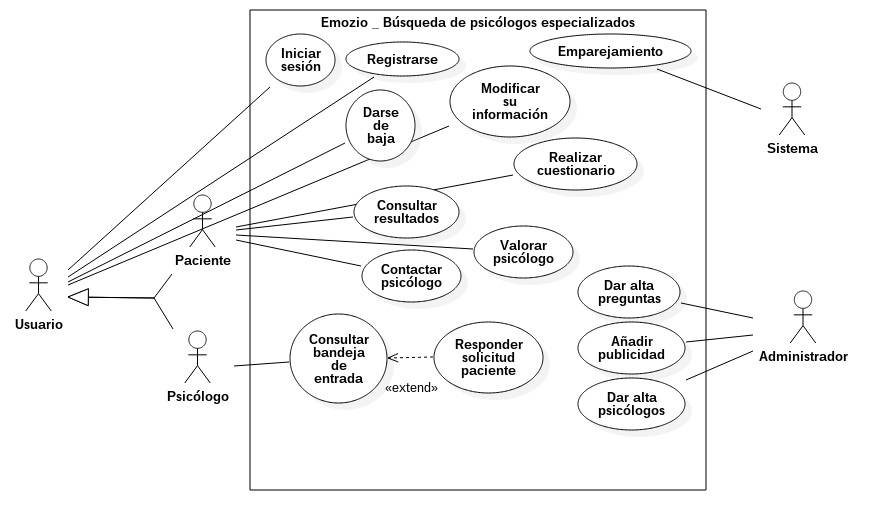
\includegraphics[width=1\textwidth]{figuras/diag_casos_uso.png}
    \caption{Diagrama de casos de uso}
    \label{fig:diag_casos_uso}
\end{figure}	

%%%%%%%%%%%%%%%%%%%%%%%%%%%%%%%%%%%%%%%%%%%%%%%%%%%%%%%%%%%%%%%%%%%%%%%%%%%%%%%%%%%%%%%
%%MODELO DE DATOS%%%%%%%%%%%%%%%%%%%%%%%%%%%%%%%%%%%%%%%%%%%%%%%%%%%%%%%%%%%%%%%%%%%%%%
%%%%%%%%%%%%%%%%%%%%%%%%%%%%%%%%%%%%%%%%%%%%%%%%%%%%%%%%%%%%%%%%%%%%%%%%%%%%%%%%%%%%%%%

\subsection{Modelado de datos}
Si los requisitos del \textit{software} incluyen la necesidad de crear, ampliar o hacer interfaz con una base de datos, o si deben construirse y manipularse estructuras de datos complejas, se debe crear un modelo de datos como parte del modelado general de los requisitos.\cite{pressman}


Los modelos semánticos de datos son la definición de la forma lógica de los datos procesados por el sistema. \cite{sommerville}


\subsubsection{¿Por qué MongoDB?}
En nuestro proyecto, los datos se encuentran almacenados en una MongoDB que consiste en una base de datos NoSQL\footnote{Las bases de datos NoSQL son aquellas que generalmente no son relacionales y no tienen un lenguaje de consulta como SQL.} de código abierto, orientada a documentos y a mantener datos desestructurados, sobretodo cuando esta crece exponencialmente. \cite{mongodb_traspas}

\subsubsection{Comparativa MongoDB con SQL}
Teniendo de referencia una base de datos SQL podemos comprender cómo MongoDB almacena la información con una pequeña analogía. En la gestión de sistemas de bases de datos relacionales, los datos se guardan en filas contenidas dentro de tablas. En cambio, en MongoDB los datos son guardados como documentos contenidos en colecciones.


Una colección es un conjunto de documentos, como éstos son independientes, pueden contener distintos campos, lo que indica que su esquema es dinámico. A su vez, estos documentos son muy similares a los JSON Objects., son conocidos como BSON objects y la principal diferencia es que contienen a mayores el tipo ObjectID que sirve de identificador del documento. Aquí es donde resaltamos una de las ventajas de utilizar MongoDB dentro de MEAN Stack, puesto que la información manejada en el lado cliente se obtiene y representa del mismo modo en el lado servidor.


En nuestro proyecto, las bases de datos son NoSQL, las cuales no tienen una representación estandarizada. Por tanto, y por entendimiento, se ha realizado a mayores una aproximación del modelo no relacional\ref{fig:mod_datos_mongoDB} al de un modelo entidad relación\ref{fig:mod_datos_mer}.

\subsubsection{Modelo de datos NoSQL}
En nuestro modelo de datos NoSQL la información está organizada en colecciones. Se debe resaltar que en algunas ocasiones, los documentos se encuentran embebidos dentro de otros. Como por ejemplo, en el caso de los comentarios de los psicólogos. Los comentarios son documentos embebidos (no tienen ObjectID) dentro de los documentos de la colección de psicólogos.


Por otra parte, están los documentos referenciados, que son independientes. Tomando el mismo ejemplo anterior, dentro de un documento embebido de comentarios hayamos una referencia a un documento de la colección de pacientes (\_idPaciente).


La estructura se ha creado de este modo porque embebiendo documentos sólo se necesitaría una única consulta, el documento en cuestión se accedería con su documento padre y las escrituras serían atómicas (no se tendrían que escribir en múltiples documentos). Pero en el caso de que el documento sea de gran relevancia y obtenga gran cantidad de información, se hará referencia a él.


\begin{figure}[htbp] 
    \centering
    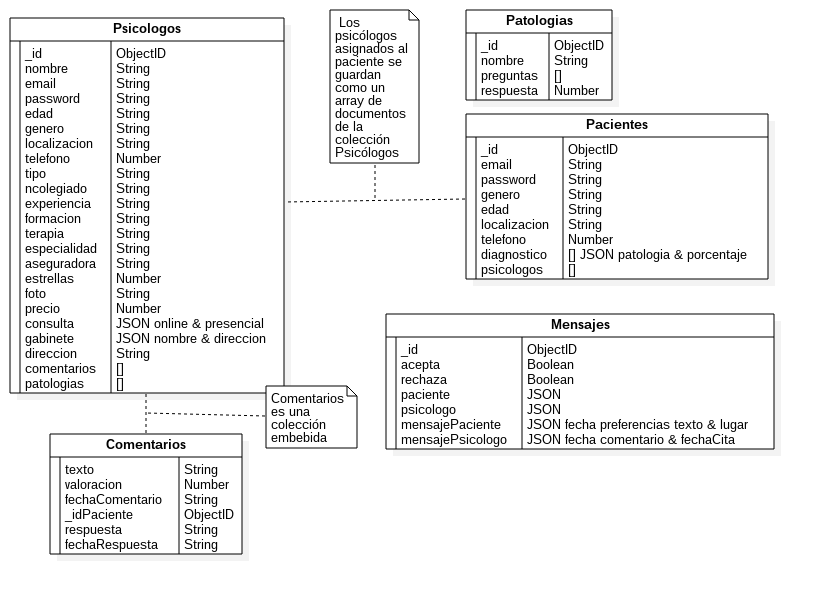
\includegraphics[width=1\textwidth]{figuras/bbdd_mod_mongoDB.png}
    \caption{Modelo de datos MongoDB}
    \label{fig:mod_datos_mongoDB}
\end{figure}	

\subsubsection{Modelo entidad-relación (MER)}
El modelo entidad-relación-atributo\ref{fig:mod_datos_mer} muestra las entidades de datos sus atributos asociados y las relaciones entre estas entidades. 


\begin{figure}[htbp] 
    \centering
    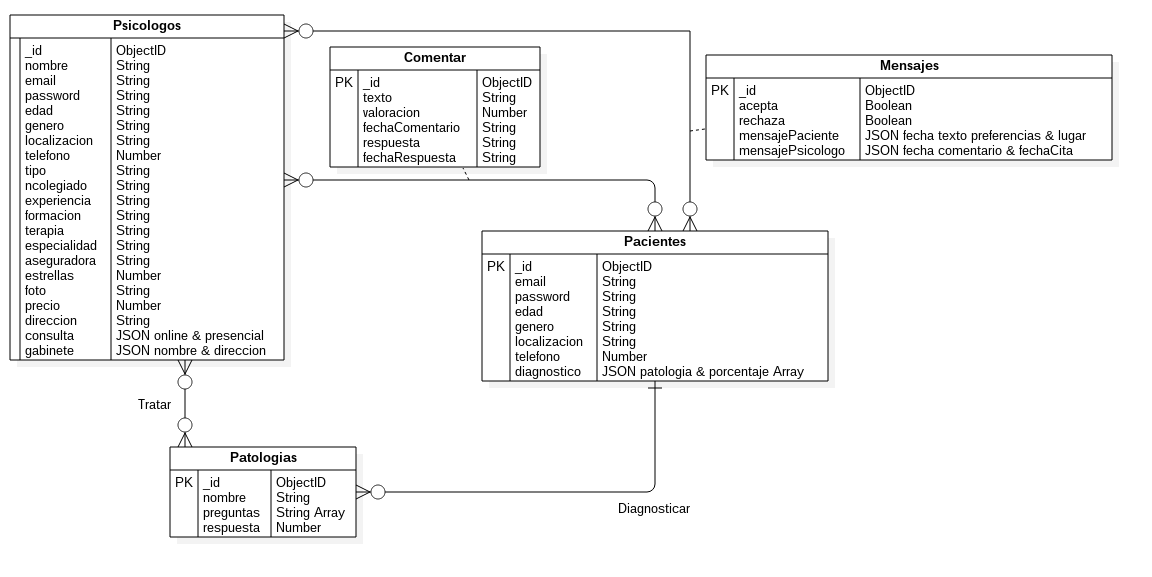
\includegraphics[width=1\textwidth]{figuras/bbdd_mod_MER.png}
    \caption{Modelo entidad-relación}
    \label{fig:mod_datos_mer}
\end{figure}

\subsubsection{Diccionario de datos}
Para mantener descripciones más detalladas de las entidades incluidas en el modelo se utilizan diccionarios de datos para gestionar toda la información.


Por tanto, un diccionario de datos es una lista de nombres ordenada alfabéticamente incluido en los modelos del sistema. Este nos proporciona un mecanismo de gestión e inventariado de nombres y sirve como un almacén de información.


\paragraph{Colecciones\ref{fig:dic_datos_colecciones}}

\begin{table}[htpb]
\centering
\begin{tabularx}{\textwidth}{|l|X|}
\hline
Colección  & Descripción                                                                               \\ \hline
Mensajes   & Almacena toda la información referente a las comunicaciones entre psicólogos y pacientes. \\ \hline
Pacientes  & Almacena toda la información sobre los pacientes del sistema.                             \\ \hline
Patologías & Almacena todas las patologías registradas hasta el momento en el sistema.                 \\ \hline
Psicólogos & Almacena toda la información sobre los psicólogos del sistema.                            \\ \hline
\end{tabularx}
\caption{Diccionario de datos: Colecciones}
\label{fig:dic_datos_colecciones}
\end{table}

\paragraph{BSON de los documentos\ref{fig:dic_datos_BSON_1}\ref{fig:dic_datos_BSON_2}\ref{fig:dic_datos_BSON_3}\ref{fig:dic_datos_BSON_4}}
\begin{table}[htpb]
\centering
\begin{tabularx}{\textwidth}{|l|X|X|X|}
\hline
Documento         & Esquema BSON                                                                                    &                                                                                  &                                                                                                                                                                                                                                  \\ \hline
                  & Campo                                                                                           & Tipo de dato                                                                     & Descripción                                                                                                                                                                                                                      \\ \hline
Mensaje           & \_id                                                                                            & ObjectID                                                                         & Identificador del documento                                                                                                                                                                                                      \\ \hline
\multirow{6}{*}{} & acepta                                                                                          & Boolean                                                                          & El psicólogo acepta la solicitud de un paciente.                                                                                                                                                                                 \\ \cline{2-4} 
                  & \begin{tabular}[c]{@{}l@{}}mensajePaciente \\ - fecha \\ - preferencias \\ - texto\end{tabular} & \begin{tabular}[c]{@{}l@{}}JSON \\ - String \\ - String \\ - String\end{tabular} & Es la información del mensaje que le envía un paciente al psicólogo. Se guarda la fecha donde fue enviado el mensaje, las preferencias horarias que tendría el paciente y el comentario que quiera transmitirle el paciente.     \\ \cline{2-4} 
                  & paciente                                                                                        & JSON                                                                             & Guarda información necesaria del documento del paciente que envió el mensaje.                                                                                                                                                    \\ \cline{2-4} 
                  & psicólogo                                                                                       & JSON                                                                             & Guarda información necesaria del documento del psicólogo que recibió el mensaje.                                                                                                                                                 \\ \cline{2-4} 
                  & rechaza                                                                                         & Boolean                                                                          & El psicólogo rechaza la solicitud de un paciente.                                                                                                                                                                                \\ \cline{2-4} 
                  & mensajePsicologo - comentario - fecha - fechaCita                                               & JSON - String - String - String                                                  & Mensaje que envía un psicólogo como respuesta a la solicitud de un paciente. Se guarda el comentario que quiera transmitirle el psicólogo, la fecha en que fué enviado el mensaje y la fecha de la cita en caso de que se la dé. \\ \hline
\end{tabularx}
\caption{Diccionario de datos: BSON Documento Mensaje}
\label{fig:dic_datos_BSON_1}
\end{table}

\begin{table}[htpb]
\centering
\begin{tabularx}{\textwidth}{|l|X|X|X|X|}
\hline
Documento         & Esquema BSON                                                                       &                                                                          &                                                                                                                                                                                  \\ \hline
                  & Campo                                                                              & Tipo de dato                                                             & Descripción                                                                                                                                                                      \\ \hline
Paciente          & \_id                                                                               & ObjectID                                                                 & Identificador del documento.                                                                                                                                                     \\ \hline
\multirow{8}{*}{} & edad                                                                               & String                                                                   & Fecha de nacimiento del psicólogo.                                                                                                                                               \\ \cline{2-4} 
                  & email                                                                              & String                                                                   & E-mail del paciente.                                                                                                                                                             \\ \cline{2-4} 
                  & Genero                                                                             & String                                                                   & Género del paciente.                                                                                                                                                             \\ \cline{2-4} 
                  & \begin{tabular}[c]{@{}l@{}}diagnostico \\ - porcentaje \\ - patologia\end{tabular} & \begin{tabular}[c]{@{}l@{}}Array JSON \\ - Number \\ - BSON\end{tabular} & Diagnóstico resultado del cuestionario. Cada documento embebido en el array está definido por el porcentaje que tiene en una patología e información necesaria de esa patología. \\ \cline{2-4} 
                  & localizacion                                                                       & String                                                                   & Ciudad donde reside el paciente.                                                                                                                                                 \\ \cline{2-4} 
                  & password                                                                           & String                                                                   & Contraseńa de la cuenta de usuario del paciente.                                                                                                                                 \\ \cline{2-4} 
                  & psicologos                                                                         & Array BSON                                                               & Conjunto de información de los psicólogos que le son asignados al paciente.                                                                                                      \\ \cline{2-4} 
                  & telefono                                                                           & Number                                                                   & Teléfono del paciente.                                                                                                                                                           \\ \hline
\end{tabularx}
\caption{Diccionario de datos: BSON Documento Paciente}
\label{fig:dic_datos_BSON_2}
\end{table}

\begin{table}[htpb]
\centering
\begin{tabularx}{\textwidth}{|l|X|X|X|X|}
\hline
Documento         & Esquema BSON &              &                                                           \\ \hline
                  & Campo        & Tipo de dato & Descripción                                               \\ \hline
Patología         & \_id         & ObjectID     & Identificador del documento.                              \\ \hline
\multirow{3}{*}{} & nombre       & String       & Nombre de la patología.                                   \\ \cline{2-4} 
                  & preguntas    & Array String & Conjunto de preguntas sobre los síntomas de la patología. \\ \cline{2-4} 
                  & respuesta    & Number       & Valor de una pregunta.                                    \\ \hline
\end{tabularx}
\caption{Diccionario de datos: BSON Documento Patología}
\label{fig:dic_datos_BSON_3}
\end{table}

\begin{table}[htpb]
\centering
\begin{tabularx}{\textwidth}{|l|X|X|X|X|}
\hline
Documento          & Esquema BSON                                                                                                                                           &                                                                                                                            &                                                                                                                                                                                                                                                                             \\ \hline
                   & Campo                                                                                                                                                  & Tipo de dato                                                                                                               & Descripción                                                                                                                                                                                                                                                                 \\ \hline
Psicólogo         & \_id                                                                                                                                                   & ObjectID                                                                                                                   & Identificador del documento.                                                                                                                                                                                                                                                \\ \hline
\multirow{18}{*}{} & aseguradora                                                                                                                                            & String                                                                                                                     & Aseguradora para la que trabaja el psicólogo.                                                                                                                                                                                                                               \\ \cline{2-4} 
                   & \begin{tabular}[c]{@{}l@{}}comentarios \\ - \_idPaciente\\ - fechaComentario\\ - fechaRespuesta \\ - respuesta \\ - texto \\ - valoracion\end{tabular} & \begin{tabular}[c]{@{}l@{}}Array JSON \\ - ObjectID \\ - String \\ - String \\ - String\\ - String\\ - Number\end{tabular} & Comentario del paciente y respuesta del psicólogo al comentario. Se guarda el identificador del paciente, la fecha en la que fue enviado, la fecha en la que fue respondido, la respuesta del psicólogo, el comentario del paciente y la valoración que le dá al psicólogo. \\ \cline{2-4} 
                   & \begin{tabular}[c]{@{}l@{}}consulta \\ - online \\ - presencial\end{tabular}                                                                           & \begin{tabular}[c]{@{}l@{}}JSON \\ - Boolean\\ - Boolean\end{tabular}                                                      & Indica si el psicólogo hace consultas presenciales, a distancia o ambas.                                                                                                                                                                                                    \\ \cline{2-4} 
                   & edad                                                                                                                                                   & String                                                                                                                     & Fecha de nacimiento del psicólogo.                                                                                                                                                                                                                                          \\ \cline{2-4} 
                   & email                                                                                                                                                  & String                                                                                                                     & E-mail del psicólogo.                                                                                                                                                                                                                                                       \\ \cline{2-4} 
                   & estrellas                                                                                                                                              & Number                                                                                                                     & Valoración media de los pacientes del psicólogo.                                                                                                                                                                                                                            \\ \cline{2-4} 
                   & experiencia                                                                                                                                            & String                                                                                                                     & Experiencia laboral del psicólogo.                                                                                                                                                                                                                                          \\ \cline{2-4} 
                   & formacion                                                                                                                                              & String                                                                                                                     & Formación del psicólogo.                                                                                                                                                                                                                                                    \\ \cline{2-4} 
                   & foto                                                                                                                                                   & String                                                                                                                     & Foto del psicólogo.                                                                                                                                                                                                                                                         \\ \cline{2-4} 
                   & localizacion                                                                                                                                           & String                                                                                                                     & Ciudad donde reside el psicólogo.                                                                                                                                                                                                                                            \\ \hline
\end{tabularx}
\caption{Diccionario de datos: BSON Documento Psicólogo - Parte 1}
\label{fig:dic_datos_BSON_4}
\end{table}

\begin{table}[htpb]
\centering
\begin{tabularx}{\textwidth}{|l|X|X|X|X|}
\hline
Documento          & Esquema BSON                                                                                                                                           &                                                                                                                            &                                                                                                                                                                                                                                                                             \\ \hline
                   & Campo                                                                                                                                                  & Tipo de dato                                                                                                               & Descripción                                                                                                                                                                                                                                                                 \\ \hline
Psicólogo         & patologias                                                                                                                                             & Array String                                                                                                               & Conjunto de nombres de las patologías que trata el psicólogo.                                                                                                                                                                                                               
\\ \cline{2-4} 
                   & ncolegiado                                                                                                                                             & String                                                                                                                     & Número de colegiado del psicólogo.                                                                                                                                                                                                                                          \\ \cline{2-4} 
                   & nombre                                                                                                                                                 & String                                                                                                                     & Nombre del psicólogo.                                                                                                                                                                                                                                                       \\ \cline{2-4} 
                   & password                                                                                                                                               & String                                                                                                                     & Contraseńa de la cuenta de usuario del psicólogo.                                                                                                                                                                                                                          
\\ \cline{2-4} 
                   & precio                                                                                                                                                 & Number                                                                                                                     & Precio de la primera consulta que dé el psicólogo.                                                                                                                                                                                                                          \\ \cline{2-4} 
                   & telefono                                                                                                                                               & Number                                                                                                                     & Teléfono del psicólogo.                                                                                                                                                                                                                                                     \\ \cline{2-4} 
                   & terapia                                                                                                                                                & String                                                                                                                     & Tipo de terapia que realiza el psicólogo.                                                                                                                                                                                                                                   \\ \cline{2-4} 
                   & tipo                                                                                                                                                   & String                                                                                                                     & Tipo del psicólogo.                                                                                                                                                                                                                                                         \\ \hline
\end{tabularx}
\caption{Diccionario de datos: BSON Documento Psicólogo - Parte 2}
\label{fig:dic_datos_BSON_4}
\end{table}

%%%%%%%%%%%%%%%%%%%%%%%%%%%%%%%%%%%%%%%%%%%%%%%%%%%%%%%%%%%%%%%%%%%%%%%%%%%%%%%%%%%%%%%
%%ANÁLISIS DE REQUISITOS%%%%%%%%%%%%%%%%%%%%%%%%%%%%%%%%%%%%%%%%%%%%%%%%%%%%%%%%%%%%%%%
%%%%%%%%%%%%%%%%%%%%%%%%%%%%%%%%%%%%%%%%%%%%%%%%%%%%%%%%%%%%%%%%%%%%%%%%%%%%%%%%%%%%%%%

\subsection{Análisis de requisitos}


Los requisitos para un sistema son la descripción de los servicios proporcionados por el sistema sus restricciones operativas y reflejan las necesidades de los clientes \cite{sommerville}.


Para poder evaluar corréctamente los requisitos, se debe definir su escala de estabilidad\ref{esc_estab} \cite{sommerville}.


\begin{table}[htpb]
\centering
\begin{tabularx}{\textwidth}{|l|X|}
\hline
ESCALA   & DESCRIPCIÓN                                                 \\ \hline
Baja     & El requisito puede sufrir cambios con facilidad             \\ \hline
Media    & Existe cierto grado de ocurrencia al cambio en el requisito \\ \hline
Alta     & La probabilidad de cambios en el requisito es muy baja      \\ \hline
Muy Alta & La probabilidad de cambios es casi nula                     \\ \hline
\end{tabularx}
\caption{Escala de estabilidad de los requisitos}
\label{esc_estab}
\end{table}


\subsubsection{Requisitos de información}


Los requisitos de información guardan toda la información que debe almacenar el sistema para poder cumplir con sus objetivos. Identifican el concepto relevante sobre el que guardar información así como qué datos específicos del concepto son importantes.


\begin{table}[htpb]
\centering
\begin{tabularx}{\textwidth}{|l|X|}
\hline
RI-001            & Paciente                                                                       \\ \hline
Descripción       & El sistema deberá almacenar la información correspondiente a los pacientes.    \\ \hline
Datos específicos & E-mail                                                                         \\ 
\multirow{8}{*}{} & Contraseńa                                                                     \\ 
                  & Género                                                                         \\ 
                  & Edad                                                                           \\ 
                  & Localización                                                                   \\ 
                  & Teléfono                                                                       \\  
                  & Síntomas                                                                       \\ 
                  & Diagnóstico                                                                    \\  
                  & Psicólogos que pueden tratar su caso \\ \hline
Estabilidad       & Media                                                                          \\ \hline
\end{tabularx}
\caption{RI-001 Paciente}
%\label{my-label}
\end{table}


\begin{table}[htpb]
\centering
\begin{tabularx}{\textwidth}{|l|X|}
\hline
RI-002            & Patología                                                                    \\ \hline
Descripción       & El sistema deberá almacenar la información correspondiente a las patologías. \\ \hline
Datos específicos & Nombre                                                                       \\ 
                  & Síntomas                                                                     \\ \hline
Estabilidad       & Alta                                                                         \\ \hline
\end{tabularx}
\caption{RI-002 Patología}
%\label{my-label}
\end{table}


\begin{table}[htpb]
\centering
\begin{tabularx}{\textwidth}{|l|X|}
\hline
RI-003             & Psicólogo                                                                    \\ \hline
Descripción        & El sistema deberá almacenar la información correspondiente a los psicólogos. \\ \hline
Datos específicos  & Nombre                                                                       \\ \hline
\multirow{18}{*}{} & E-mail                                                                       \\ 
                   & Contraseńa                                                                   \\  
                   & Género                                                                       \\ 
                   & Edad                                                                         \\  
                   & Localización                                                                 \\ 
                   & Teléfono                                                                     \\ 
                   & Tipo                                                                         \\ 
                   & Número                                                                       \\  
                   & Experiencia                                                                  \\ 
                   & Formación                                                                    \\ 
                   & Terapia                                                                      \\ 
                   & Especialidad                                                                 \\ 
                   & Aseguradora                                                                  \\  
                   & Patologías                                                                   \\  
                   & Valoración                                                                   \\ 
                   & Precio                                                                       \\ 
                   & Tipo de consulta: Online o presencial                                        \\
                   & Gabinete                                                                     \\ \hline
Estabilidad        & Media                                                                        \\ \hline
\end{tabularx}
\caption{RI-003 Psicólogo}
%\label{my-label}
\end{table}


\subsubsection{Requisitos funcionales}


Los requisitos funcionales son declaraciones de los servicios que debe proporcionar el sistema. Los requisitos funcionales se encuentran divididos en función de los incrementos donde vayan a implementarse\cite{sommerville}.


%\paragraph{Gestión de usuarios}


\begin{table}[htpb]
\centering
\begin{tabularx}{\textwidth}{|l|X|}
\hline
RF - 001                                & Acceso usuarios                                                                                              \\ \hline
Descripción                             & Cualquier usuario registrado en la plataforma podrá acceder a la plataforma a través de la página de acceso. \\ \hline
Estabilidad                             & Alta                                                                                                         \\ \hline
Dependencias & \begin{tabular}[c]{@{}l@{}}RI-001 \\ RI-003 \\ RF-002\end{tabular}                                           \\ \hline
\end{tabularx}
\caption{RF-001 Acceso usuarios}
%\label{my-label}
\end{table}


\begin{table}[htpb]
\centering
\begin{tabularx}{\textwidth}{|l|X|}
\hline
RF - 002                                & Registro                                                                                                        \\ \hline
Descripción                             & Cualquier usuario podrá acceder a los servicios de la plataforma tras haber cubierto el formulario de registro. \\ \hline
Estabilidad                             & Alta                                                                                                            \\ \hline
Dependencias & \begin{tabular}[c]{@{}l@{}}RI-001\\ RI-003\end{tabular}                                                         \\ \hline
\end{tabularx}
\caption{RF-002 Registro}
%\label{my-label}
\end{table}


\begin{table}[htpb]
\centering
\begin{tabularx}{\textwidth}{|l|X|}
\hline
RF - 003                                & Baja                                                                                \\ \hline
Descripción                             & Cualquier usuario registrado en la plataforma podrá darse de baja de la plataforma. \\ \hline
Estabilidad                             & Alta                                                                                \\ \hline
Dependencias & \begin{tabular}[c]{@{}l@{}}RI-001\\ RI-003\\ RF-002\end{tabular}                    \\ \hline
\end{tabularx}
\caption{RF-003 Baja}
%\label{my-label}
\end{table}


\begin{table}[htpb]
\centering
\begin{tabularx}{\textwidth}{|l|X|}
\hline
RF - 004                                & Modificación de los datos                                                           \\ \hline
Descripción                             & Cualquier usuario registrado en la plataforma podrá modificar sus datos de usuario. \\ \hline
Estabilidad                             & Alta                                                                                \\ \hline
Dependencias & \begin{tabular}[c]{@{}l@{}}RI-001\\ RI-003\\ RF-001\\ RF-002\end{tabular}           \\ \hline
\end{tabularx}
\caption{RF-004 Modificación de los datos}
%\label{my-label}
\end{table}

%\paragraph{Cuestionario/Emparejamiento}


\begin{table}[htpb]
\centering
\begin{tabularx}{\textwidth}{|l|X|}
\hline
RF - 005                                & Emparejamiento                                                                                                                                                                                                                                                                     \\ \hline
Descripción                             & Se garantizará al paciente el emparejamiento con el psicólogo más adecuado para tratar su caso. Cualquier paciente registrado en la plataforma podrá especificar sus síntomas a través de un cuestionario asignándole al menos un psicólogo al paciente tras conocer su patología. \\ \hline
Estabilidad                             & Alta                                                                                                                                                                                                                                                                               \\ \hline
Dependencias & \begin{tabular}[c]{@{}l@{}}RI-001\\ RI-002\\ RI-003\\ RF-001\\ RF-002\end{tabular}                                                                                                                                                                                                 \\ \hline
\end{tabularx}
\caption{RF-005 Emparejamiento}
%\label{my-label}
\end{table}

\begin{table}[htpb]
\centering
\begin{tabularx}{\textwidth}{|l|X|}
\hline
RF - 006                                & Filtrado de los resultados en base a distintos criterios                                                                                                                                              \\ \hline
Descripción                             & Cualquier paciente, que haya obtenido resultados concluyentes en el cuestionario, podrá  filtrarlos en base a distintos criterios como las características geográficas, el precio o su seguro médico. \\ \hline
Estabilidad                             & Alta                                                                                                                                                                                                  \\ \hline
Dependencias & \begin{tabular}[c]{@{}l@{}}RI-003\\ RF-001\\ RF-002\\ RF-005\end{tabular}                                                                                                                             \\ \hline
\end{tabularx}
\caption{RF-006 Filtrado de los resultados en base a distintos criterios}                                                                                                                                          
%\label{my-label}
\end{table}

%\paragraph{Comunicación/Valoraciones/Comentario}


\begin{table}[htpb]
\centering
\begin{tabularx}{\textwidth}{|l|X|}
\hline
RF - 007                                & Contacto del paciente con el psicólogo                                                                               \\ \hline
Descripción                             & El paciente podrá contactar con cualquiera de los psicólogos que le fueron  asignados tras realizar el cuestionario. \\ \hline
Estabilidad                             & Alta                                                                                                                 \\ \hline
Dependencias & \begin{tabular}[c]{@{}l@{}}RI-001\\ RI-003\\ RF-001\\ RF-002\\ RF-005\end{tabular}                                   \\ \hline
\end{tabularx}
\caption{RF-007 Contacto del paciente con el psicólogo}                                                                                                                                          
%\label{my-label}
\end{table}

\clearpage

\begin{table}[htpb]
\centering
\begin{tabularx}{\textwidth}{|l|X|}
\hline
RF - 008                                & Valoración del psicólogo por parte del paciente                                    \\ \hline
Descripción                             & El paciente podrá valorar al psicólogo que le haya atendido.                       \\ \hline
Estabilidad                             & Alta                                                                               \\ \hline
Dependencias & \begin{tabular}[c]{@{}l@{}}RI-001\\ RI-003\\ RF-001\\ RF-002\\ RF-005\end{tabular} \\ \hline
\end{tabularx}
\caption{RF-008 Valoración del psicólogo por parte del paciente}                                                                                                                                                                            
%\label{my-label}
\end{table}


\subsubsection{Requisitos no funcionales}


Los requisitos no funcionales son restricciones de los servicios o funciones ofrecidos por el sistema. Incluyen restrucciones de tiempo, sobre el proceso de desarrollo y estándares\cite{sommerville}.

\begin{table}[htpb]
\centering
\begin{tabularx}{\textwidth}{|l|X|}
\hline
RNF - 001                               & Encriptado de datos                                                                                            \\ \hline
Descripción                             & Los datos de los pacientes almacenados en la base de datos deberán estar cifrados con un algoritmo de cifrado. \\ \hline
Estabilidad                             & Alta                                                                                                           \\ \hline
Dependencias & (Es transversal)                                                                                               \\ \hline
\end{tabularx}
\caption{RNF-001 Encriptado de datos}                                                                                                                                                                                                                                                                      
%\label{my-label}
\end{table}

\clearpage

\begin{table}[htpb]
\centering
\begin{tabularx}{\textwidth}{|l|X|}
\hline
RNF - 002                               & Tiempo de respuesta de asignación                                                                                                                                            \\ \hline
Descripción                             & El paciente tras enviar las respuestas del cuestionario, los resultados de asignación de psicólogo del mismo deberán tener un tiempo de respuesta de como máximo 5 segundos. \\ \hline
Estabilidad                             & Alta                                                                                                                                                                         \\ \hline
Dependencias & RF-005                                                                                                                                                                       \\ \hline
\end{tabularx}
\caption{RNF-002 Tiempo de respuesta de asignación}                                                                                                                                                                                                                                                                      
%\label{my-label}
\end{table}


\subsubsection{Matrices de rastreabilidad}

El rastreo es una propiedad de la especificación de requisitos que refleja la facilidad de encontrar requisitos relacionados. Es importante ya que nos da a conocer las relaciones que hay entre éstos y el diseño del sistema, y así, si se proponen cambios, se podrá rastrear cuál es el impacto de esos cambios en los otros requisitos y en el diseño del sistema.


\paragraph{Matriz de rastreabilidad: RF / RI\ref{mat_rast_rf_ri}}

\begin{table}[htpb]
\centering
\begin{tabular}{|l|l|l|l|l|}
\hline
\multicolumn{2}{|l|}{\multirow{2}{*}{}} & \multicolumn{3}{l|}{Requisitos de información} \\ \cline{3-5} 
\multicolumn{2}{|l|}{}                  & RI-001         & RI-002        & RI-003        \\ \hline
Requisitos funcionales     & RF-001     & X              &               & X             \\ \hline
\multirow{7}{*}{}          & RF-002     & X              &               & X             \\ \cline{2-5} 
                           & RF-003     & X              &               & X             \\ \cline{2-5} 
                           & RF-004     & X              &               & X             \\ \cline{2-5} 
                           & RF-005     & X              & X             & X             \\ \cline{2-5} 
                           & RF-006     &                &               & X             \\ \cline{2-5} 
                           & RF-007     & X              &               & X             \\ \cline{2-5} 
                           & RF-008     & X              &               & X             \\ \hline
\end{tabular}
\caption{Matriz de rastreabilidad: RF / RI}
\label{mat_rast_rf_ri}
\end{table}


\paragraph{Matriz de rastreabilidad: CU / RF\ref{mat_rast_cu_rf}}

\begin{table}[htpb]
\centering
\begin{tabularx}{\textwidth}{|l|X|X|X|X|X|X|X|X|}
\hline
\multicolumn{2}{|l|}{\multirow{2}{*}{}} & \multicolumn{7}{l|}{Requisitos funcionales}                  \\ \cline{3-9} 
\multicolumn{2}{|l|}{}                  & RF-001 & RF-002 & RF-003 & RF-004 & RF-005 & RF-006 & RF-007 \\ \hline
Casos de uso             & CU-001       & X      &        &        &        &        &        &        \\ \hline
\multirow{15}{*}{}       & CU-002       & X      & X      &        &        &        &        &        \\ \cline{2-9} 
                         & CU-003       & X      & X      &        &        & X      &        &        \\ \cline{2-9} 
                         & CU-004       & X      & X      &        &        & X      & X      &        \\ \cline{2-9} 
                         & CU-005       & X      & X      &        &        & X      &        &        \\ \cline{2-9} 
                         & CU-006       & X      & X      &        &        &        &        &        \\ \cline{2-9} 
                         & CU-007       & X      & X      &        &        & X      &        & X      \\ \cline{2-9} 
                         & CU-008       & X      & X      &        &        & X      &        &        \\ \cline{2-9} 
                         & CU-009       & X      & X      &        &        & X      &        &        \\ \cline{2-9} 
                         & CU-010       & X      & X      &        &        &        &        &        \\ \cline{2-9} 
                         & CU-011       & X      &        &        &        &        &        &        \\ \cline{2-9} 
                         & CU-012       & X      &        &        &        &        &        &        \\ \cline{2-9} 
                         & CU-013       & X      & X      &        &        & X      &        &        \\ \cline{2-9} 
                         & CU-014       &        &        &        &        &        &        &        \\ \cline{2-9} 
                         & CU-015       &        &        &        &        &        &        &        \\ \cline{2-9} 
                         & CU-016       &        &        &        &        &        &        &        \\ \hline
\end{tabularx}
\caption{Matriz de rastreabilidad: CU / RF}
\label{mat_rast_cu_rf}
\end{table}

%%%%%%%%%%%%%%%%%%%%%%%%%%%%%%%%%%%%%%%%%%%%%%%%%%%%%%%%%%%%%%%%%%%%%%%%%%%%%%%%%%%%%%%
%ALGORITMO MATCHING%%%%%%%%%%%%%%%%%%%%%%%%%%%%%%%%%%%%%%%%%%%%%%%%%%%%%%%%%%%%%%%%%%%
%%%%%%%%%%%%%%%%%%%%%%%%%%%%%%%%%%%%%%%%%%%%%%%%%%%%%%%%%%%%%%%%%%%%%%%%%%%%%%%%%%%%%%%

\subsection{Algoritmo de \textit{matching}}


Para poder emparejar al psicólogo que puede tratar la patología de un paciente, se ha diseñado el algoritmo descrito a continuación. Como el estudio del test validado científicamente que determina cómo se van a evaluar las patologías, pacientes y psicólogos en cuestión no está diseñado todavía, se ha tenido que realizar una breve y pequeña aproximación de cómo sería el funcionamiento aparente del cuestionario.


En nuestro proyecto, cada patología tendrá asociadas una serie de preguntas. La respuesta a todas las preguntas nos dará una ponderación de valor 1. En el conjunto de las posibles preguntas de una patología, existirá una pregunta principal cuyo valor es 0,5, y el valor de cada una del resto, viene dado por la siguiente fórmula:

\begin{equation}
\frac{1}{2}\times\frac{1}{n_{preguntas}-1}+\frac{1}{2}\times{valor_{preg_{princ}}} = 1
\label{mi_ecuacion}
\end{equation}
%
%
%½ * (1/(nº preguntas-1)) + ½ * pregunta principal = 1
%
%
Teniendo en cuenta esto, el test de la plataforma está dividido en dos partes:


La primera, muestra la pregunta más relevante de cada patología estimada por nuestro experto psicólogo. En el momento que el paciente indica que tiene el síntoma especificado en la pregunta A (correspondiente a la patología A), se le diagnosticará que posee la patología A con una ponderación del 0,5.


La segunda, muestra las preguntas restantes a las patologías marcadas en la primera parte, es decir, aquellas patologías que le han sido diagnosticadas con una ponderación del 0,5. Por cada pregunta marcada en la segunda parte, se sumará el valor de esa pregunta al porcentaje actual.


Una vez enviado el formulario, sólo si el porcentaje es mayor o igual al 0,7, se determina que el paciente padece esa patología.


\paragraph{Un ejemplo práctico\ref{ej_alg_match}}


\begin{figure}[htbp] 
    \centering
    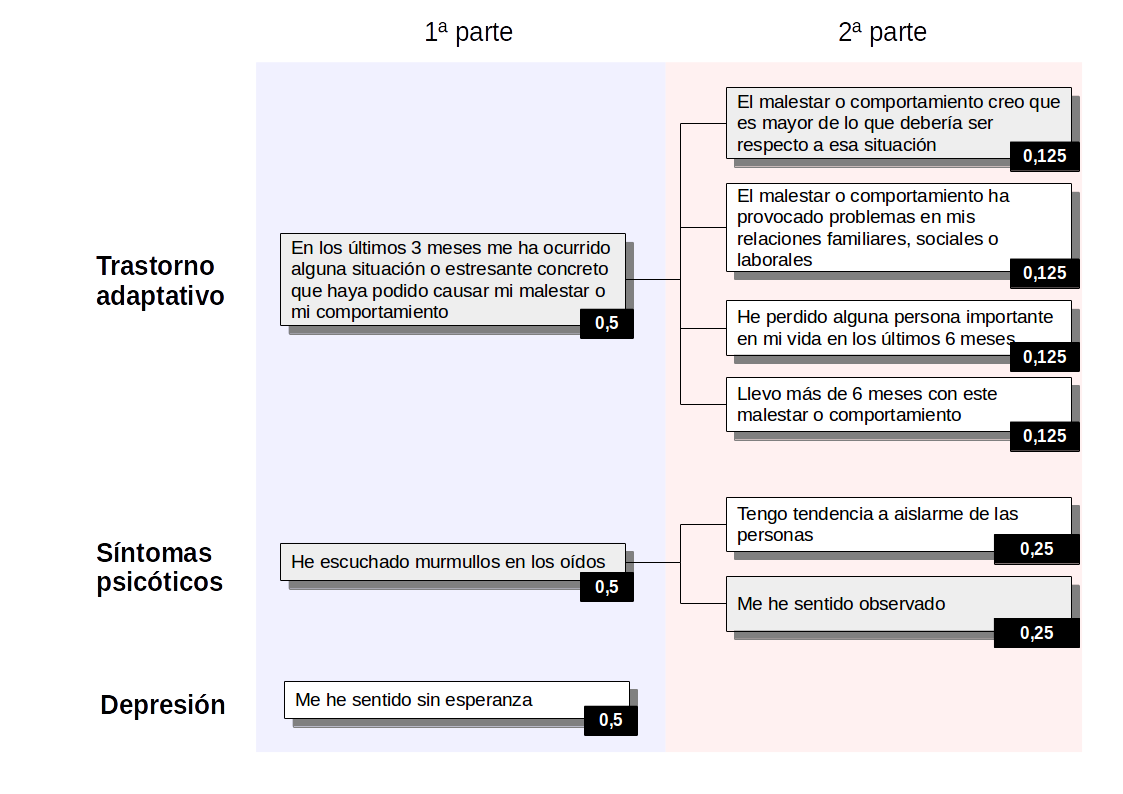
\includegraphics[width=1\textwidth]{figuras/alg_matching.png}
    \caption{Ejemplo algoritmo de \textit{matching}}
    \label{ej_alg_match}
\end{figure}	

Si el paciente marcase las preguntas que aparecen en color gris, en la segunda parte del test aparecerían el resto de preguntas de la patología en cuestión.


Tras finalizar el test, los resultados serían:

\begin{itemize}
\item Trastorno adaptativo 0,625: Se descartaría.
\item Síntomas psicóticos 0,75
\end{itemize}

%%%%%%%%%%%%%%%%%%%%%%%%%%%%%%%%%%%%%%%%%%%%%%%%%%%%%%%%%%%%%%%%%%%%%%%%%%%%%%%%%%%%%%%
%TECNOLOGÍAS UTILIZADAS%%%%%%%%%%%%%%%%%%%%%%%%%%%%%%%%%%%%%%%%%%%%%%%%%%%%%%%%%%%%%%%%
%%%%%%%%%%%%%%%%%%%%%%%%%%%%%%%%%%%%%%%%%%%%%%%%%%%%%%%%%%%%%%%%%%%%%%%%%%%%%%%%%%%%%%%

%\subsection{Tecnologías utilizadas}
%
%\subsubsection{\textit{Frameworks}}
%Un \textit{framework} es una arquitectura de software que modela las relaciones generales de las entidades del dominio, y provee una estructura y una especial metodología de trabajo, la cual extiende o utiliza las aplicaciones del dominio.
%
%
%Los frameworks involucrados en nuestro proyecto son MEAN Stack, Bootstrap y Semantic UI.
%
%\paragraph{MEAN Stack}
%Es un \textit{framework} para el desarrollo de aplicaciones, y páginas web dinámicas, basadas en JavaScript: MongoDB, ExpressJS, AngularJS y NodeJS, lo cual permite que se integren entre ellas eficazmente.
%
%
%Con MongoDB podemos almacenar nuestros documentos en formato JSON, se pueden escribir consultas en nuestro servidor ExpressJS y NodeJS, y del mismo modo, pasar esos documentos JSON a nuestro \textit{frontend} hecho con AngularJS.
%
%
%El \textit{debugging} y la administración de la base de datos se vuelven más sencillas cuando el objeto almacenado en la base de datos es idéntico al objeto que tu cliente JavaScript puede ver\cite{mongodb_blog_mean_stack}.
%
%
%Algunos de los motivos por los que escogí este \textit{framework} es por su escalabilidad, rapidez y flexibilidad, ya que permite que en un futuro sea sencillo poder adaptar la aplicación a plataformas móviles, o añadir cambios con facilidad.
%
%
%Los componentes que forman el \textit{framework} son:
%
%\begin{itemize}
%\item \textbf{MongoDB}
%MongoDB es una base de datos ágil NoSQL orientada a documentos que permite que los esquemas cambien rápidamente a medida que las aplicaciones evolucionan, proporcionando siempre la funcionalidad que los desarrolladores esperan de las bases de datos tradicionales, tales como índices secundarios, un lenguaje completo de búsquedas y consistencia. En resumen, MongoDB brinda escalabilidad, rendimiento y gran disponibilidad. \cite{mongodb}
%\item \textbf{ExpressJS}
%ExpressJS es una middleware de aplicaciones web Node.js minimalista y flexible que proporciona un conjunto sólido de características para aplicaciones web y móviles. Se trata de una API REST que utiliza métodos HTTP para obtener datos o generar operaciones sobre esos datos. \cite{expressjs}
%\item \textbf{AngularJS}
%AngularJS es un framework para construir client applications en HTML y Javascript, aunque también puede ser otro lenguaje como TypeScript que sea compilado a JavaScript. El framework posee un conjunto de librerías funcionales, y otras opcionales. \cite{angularjs_arch}
%Angular permite fácilmente construir aplicaciones web, ya que combina \textit{declarative templates}, \textit{dependency injection} y \textit{end to end tooling}, e integra buenas prácticas de programación. Las aplicaciones desarrolladas con Angular funcionan tanto para web, móvil o escritorio. \cite{angularjs_docs}
%\item \textbf{NodeJS}
%NodeJS es un entorno de ejecución para JavaScript construido con el motor de JavaScript V8 de Chrome. Node.js usa un modelo de operaciones entrada/salida sin bloqueo (asíncrono) y orientado a eventos, que lo hace liviano y eficiente, ya que nunca se bloquea. 
%Node está diseñado sin hilos, este presenta un bucle de eventos como un entorno en vez de una librería. Node simplemente ingresa el bucle de eventos después de ejecutar el script de entrada. Node sale del bucle de eventos cuando no hay más callbacks que ejecutar. \cite{nodejs_about}
%\end{itemize}
%
%
%\paragraph{Bootstrap}
%Bootstrap es un \textit{framework} de código abierto para desarrollar con HTML, CSS y JS. Contiene características como un grid responsive, docenas de componentes, JavaScript plugins, tipografía, control de formularios y capacidad de personalización.\cite{bootstrap_get}
%
%
%\paragraph{Semantic UI}
%Semantic UI es un \textit{framework} que permite a los desarrolladores contruir rápidamente sitios web, con HTML conciso, JavaScript intuitivo, y simplicando el \textit{debugging}. Semantic está diseñado de manera responsive permitiendo que la aplicación sea escalable en múltiples dispositivos. Semantic está preparado para poder asociarse con otros \textit{frameworks} como React, Angular, Meteor y Ember. \cite{semanticui_github}
%
%
%\subsection{Lenguajes de programación}





%\cleardoublepage
%DISEÑO
%\chapter{Diseño}

%%%%%%%%%%%%%%%%%%%%%%%%%%%%%%%%%%%%%%%%%%%%%%%%%%%%%%%%%%%%%%%%%%%%%%%%%%%%%%%%%%%%%%
%%%%%%%%%%%%%%%%%%%%%%%%%%%%%%%%%%%%%%%%%%%%%%%%%%%%%%%%%%%%%%%%%%%%%%%%%%%%%%%%%%%%%%
%DISEÑO DE LA INTERFAZ
%%%%%%%%%%%%%%%%%%%%%%%%%%%%%%%%%%%%%%%%%%%%%%%%%%%%%%%%%%%%%%%%%%%%%%%%%%%%%%%%%%%%%%
%%%%%%%%%%%%%%%%%%%%%%%%%%%%%%%%%%%%%%%%%%%%%%%%%%%%%%%%%%%%%%%%%%%%%%%%%%%%%%%%%%%%%%

\section{Diseño de la interfaz}
El diseño de la interfaz de usuario crea un medio eficaz de comunicación entre los seres humanos y la computadora.


\subsection{Principios de diseño de la experiencia de usuario}
Para poder realizar un diseño de interfaz centrado en el usuario, primero hemos de conocer quiénes y cómo son nuestros usuarios. Durante el desarrollo del modelo de negocio pudimos entrevistar a nuestros posibles clientes (futuros usuarios) y pudimos hacernos una idea de cuál es nuestro nicho de mercado.


En nuestra plataforma, tenemos dos tipos de perfiles: Los pacientes\ref{perf_pac} y los psicólogos\ref{perf_psic}.


\begin{table}[htpb]
\centering
\begin{tabular}{|l|l|}
\hline
\multicolumn{2}{|c|}{\textbf{Pacientes}}                                                                                                                                                                               \\ \hline
\textbf{Demografía}                                & España                                                                                                                                                            \\ \hline
\textbf{Edad}                                      & Mayores de 16 años                                                                                                                                                \\ \hline
\textbf{Experiencia laboral}                       & Estudios mínimos                                                                                                                                                  \\ \hline
\textbf{Contexto profesional}                      & Cualquiera                                                                                                                                                        \\ \hline
\multirow{2}{*}{\textbf{Necesidades e intereses}}  & Buscar al psicólogo más adecuado para tratar su problemática.                                                                                                     \\ \cline{2-2} 
                                                   & Reducir las preocupaciones de aquellas poblaciones que no puedan acudir físicamente a una consulta por motivos de desplazamiento, urgencias, estigmas sociales... \\ \hline
\textbf{¿Cuándo y dónde utilizaran este servicio?} & Cuando surja la necesidad de contactar con un psicólogo y a través de un ordenador.                                                                               \\ \hline
\end{tabular}
\caption{Perfil paciente}
\label{perf_pac}
\end{table}


\begin{table}[htpb]
\centering
\begin{tabular}{|l|l|}
\hline
\multicolumn{2}{|c|}{\textbf{Psicólogos}}                                                                                                                                 \\ \hline
\textbf{Demografía}                                & España                                                                                                               \\ \hline
\textbf{Edad}                                      & Mayoría de edad                                                                                                      \\ \hline
\textbf{Experiencia laboral}                       & Estudios superiores                                                                                                  \\ \hline
\textbf{Contexto profesional}                      & Psicólogos con especialidad clínica o sanitaria que estean colegiados para el ejercicio de la actividad profesional. \\ \hline
\textbf{Necesidades e intereses}                   & Conseguir un flujo constante de pacientes.                                                                           \\ \hline
\textbf{¿Cuándo y dónde utilizaran este servicio?} & Periódicamente y a través de un ordenador.                                                                           \\ \hline
\end{tabular}
\caption{Perfil psicólogo}
\label{perf_psic}
\end{table}


Hacer un diseño centrado en el usuario implica tenerlo presente a lo largo de todo el proceso de diseño y tratar de entender cuáles son sus necesidades, intereses y limitaciones.


\subsection{Principios de diseño de la interfaz de usuario}

\subsubsection{\textit{Layout}}
Nuestra interfaz seguirá la regla de los tercios para ayudar a concretar el enfoque del usuario. La regla de los tercios es una forma de composición para ordenar objetos dentro de la imagen al dividirla en nueve partes iguales utilizando dos líneas imaginarias paralelas y equiespaciadas de forma horizontal y otras dos con la mismas características de forma vertical. Los puntos donde se cortan las líneas son los puntos de intersección y sirven para distribuir los elementos de la página. Entre los puntos de intersección se ha de ubicar el centro de atención para crear una imagen estéticamente agradable y equilibrada\cite{georgefield1845}.


La librería Bootstrap, que es una de las librerías escogidas para el diseño de la página, posee un sistema de cuadrículas\cite{bootstrap_grid_basic} que permite dividir la página en filas y columnas. La cuadrícula siempre divide la página en 12 columnas. Como 12 es múltiplo 3, se puede aplicar fácilmente la regla de los tercios a este sistema de cuadrículas.


Por otra parte, también se debe tener en cuenta el público que va a tener nuestra página a la hora de disponer los objetos en ella. La jerarquía visual es importante porque dirige la atención de los ojos del usuario. En nuestro caso, nuestra población es occidental, por lo que el usuario comienza a leer la página desde la esquina superior izquierda. Por este motivo, es interesante situar el logo de nuestra plataforma en esta esquina y la navegación a su lado de forma horizontal.


\subsubsection{Colores}
En la página predominan los colores que, para nuestros futuros usuarios pertenecientes a la población occidental, transmiten:


\begin{itemize}
\item Verde: Seguridad, salud
\item Azul: Seguridad, confianza, estabilidad, veracidad, lealtad
\end{itemize}


El verde y azul son colores análogos, puesto que se encuentran uno pegado a otro en la rueda de color.


Es importante tener en cuenta la cultura de nuestros usuarios, puesto que entre culturas   pueden existir connotaciones de los colores totalmente opuestas.


Para el color de las letras se han utilizado el blanco y el negro (colores neutros) y hacen contraste con el color predominante del background y de los elementos de la página.


\subsection{Fuentes y tipografía}
La tipografía predominante en toda la página es Lato\cite{lato}, pero para aquellos mensajes que queramos resaltar en algún momento puntual se utilizará Merriweather\cite{merriweather}.


La elección de las fuentes se debe a que la tipografía contextualiza el tipo de contenido de la página, no sólo lo hace a nivel verbal sino que también de forma visual. El lector, primero identifica los patrones gráficos de la página, y después, analiza el lenguaje y lee.


\begin{itemize}
\item Lato
Es de tipo \textit{sans serif}\footnote{\textbf{\textit{Sans serif}:} Fuentes con ausencia de \textit{serif}.} transicional: Los trazos son fuertes y los caracteres son derechos y uniformes. Transmite sencillez y modernez. Se suele utilizar en tecnología y aplicaciones portables.
\item Merriweather
Es de tipo egipcio (\textit{slab serif}): Existe muy poco contraste entre los trazos, y la \textit{serif} es gruesa. Transmite autoridad pero en tono amistoso. Se suele utilizar en \textit{marketing} y aplicaciones promocionales.
\end{itemize}


\subsection{Interacción persona-ordenador}
\subsubsection{Sociedad de la información}
La tendencia que existe hoy en día es digitalizar toda clase de servicios. Los servicios TIC permiten acceder a la salud, el ocio, el bienestar, la formación... derechos básicos que pertenecen a toda la ciudadanía.


A pesar de ello, existen personas que no tienen fácil acceso a este tipo de servicios ya sea por razones de limitaciones geográficas como es el caso del rural, aspectos de género culturales o religiosos, la edad, aspectos socieconómicos (personas bajo el umbral de difícil acceso a las TIC) y la discapacidad.
Aunque el proyecto no pueda abarcar a toda clase de colectivos por limitaciones de tiempo, sí es importante tenerlos en cuenta para el futuro.


\subsubsection{Diversidad funcional} 
La diversidad funcional es inherente al ser humano: Una persona experimenta variaciones en su capacidad de dependencia a lo largo de su vida, aunque sea de manera temporal. Por ejemplo, a veces nos sentimos limitados por no poder utilizar el ordenador portátil al no tener batería; o con la edad, la gente obtiene discapacidades que antes no tenía como la pérdida de vista.


\subsubsection{Accesibilidad}
La accesibilidad la interacción persona-ordenador es el conjunto de propiedades que debe incorporar un producto, servicio o sistema, de forma que el mayor número posible de personas, en el mayor número posible de circunstancias, que sea comercialmente práctico tener en cuenta, puede acceder a él y usarlo.\cite{nordic_guidelines}


Un producto es accesible si, por mucho tiempo o esfuerzo que requiera, la tarea puede realizarse.


\subsubsection{Usabilidad}
La usabilidad es la efectividad, eficiencia y satisfacción con la que usuarios específicos pueden abarcar unos objetivos determinados en un entorno particular\cite{iso_ergonomics}.


Por tanto, los sistemas deben ser usables y accesibles para que la inmensa mayoría de las personas puedan utilizarlo con calidad.


\subsubsection{Diseño universal}
El diseño universal es la estrategia que tiene como objetivo diseñar productos y servicios que puedan se utilizados por el mayor número de personas, considerando que existe una amplia variedad de habilidades humanas y no una habilidad media, sin necesidad de llevar a cabo una adaptación o diseñi especializado, simplificando la vida de todas las personas con independencia de su edad, talla o capacidad\cite{ekberg}.


En la práctica, esto supone un auténtico reto, por lo que el diseño para todos acaba equivaliendo a diseño para “la mayoría”. Aquí es donde se entra a valorar la posibilidad de añadir productos de apoyo para que pueda ser utilizado por las minorías.


En España hay leyes que tratan de combatir con este tipo de discriminación como la Ley 51/2005, de 2 de diciembre, de igualdad de oportunidades, no discriminación y accesibilidad universal de las personas con discapacidad. Por otra parte, AENOR posee la norma UNE 139803:2012. Requisitos de Accesibilidad para contenidos en la web\cite{aenor_req_acces}.


Para lograr que nuestra plataforma pueda ser utilizada por el mayor número de personas posible se ha decidido seguir los principios heurísticos de Nielsen y Molich.


\subsubsection{Principios heurísticos}
La Interacción Persona Ordenador (IPO) presenta a la Evaluación Heurística (EH) como un método de evaluación de la usabilidad por inspección que debe ser llevado a cabo a través de unos principios heurísticos previamente establecidos. Por ser un método de evaluación de la usabilidad, tiene como objetivo medir la calidad de la interfaz de cualquier sistema interactivo en relación a su facilidad para ser aprendido y usado por un determinado grupo de usuarios en un determinado contexto de uso.


Aplicar los principios heurísticos nos sirve de guía para el proceso de diseño y nos permite identificar problemas de usabilidad en las interfaces de usuario. En nuestra aplicación, tendremos en cuenta los principios heurísticos de Nielsen y Molich:


\begin{enumerate}
\item Visibilidad del estado del sistema
El sistema debe siempre mantener a los usuarios informados del estado del sistema, con una realimentación apropiada y en un tiempo razonable.
\item Lenguaje de los usuarios
El sistema debe hablar el lenguaje de los usuarios, utilizando convenciones del mundo real, disponiendo la información en un orden natural y lógico.
\item Control y libertad para el usuario
Los usuarios eligen a veces funciones del sistema por error y necesitan una salida del estado indeseado sin tener que pasar por un diálogo extendido.
\item Consistencia y estándares
Se deben seguir las normas y convencios de la plataforma para las que se implementa el sistema.
\item Ayuda a los usuarios para reconocimiento, diagnóstico y recuperación de errores
Los mensajes de error deben expresarse en un lenguaje claro y explicativo.
\item Prevención de errores
Se debe prevenir la aparición de errores que mejor que generar buenos mensajes de error.
\item Reconocimiento antes de cancelación
El usuario no debería tener que recordar la información de una parte del diálogo a la otra.
\item Flexibilidad y eficiencia de uso
Las instrucciones para el uso del sistema deben ser visibles o fácilmente accesibles siempre que se necesiten.
\item Estética de diálogos y diseño minimalista
No deben contener la información que sea inaplicable o se necesite raramente. Cada unidad adicional de la información en un diálogo compite con las unidades relevantes de la información y disminuye su visibilidad.
\item Ayuda general y documentación
Aunque es mejor si el sistema se pueda usar sin documentación, puede ser necesario disponer de ayuda y documentación. Ésta ha de ser fácil de buscar, centrada en las tareas del usuario, tener información de las etapas a realizar y que no sea muy extensa. \cite{eval_heuris}
\end{enumerate}


\subsection{\textit{Mockup}}



%%%%%%%%%%%%%%%%%%%%%%%%%%%%%%%%%%%%%%%%%%%%%%%%%%%%%%%%%%%%%%%%%%%%%%%%%%%%%%%%%%%%%%
%%%%%%%%%%%%%%%%%%%%%%%%%%%%%%%%%%%%%%%%%%%%%%%%%%%%%%%%%%%%%%%%%%%%%%%%%%%%%%%%%%%%%%
%DISEÑO DE LA NAVEGACIÓN
%%%%%%%%%%%%%%%%%%%%%%%%%%%%%%%%%%%%%%%%%%%%%%%%%%%%%%%%%%%%%%%%%%%%%%%%%%%%%%%%%%%%%%
%%%%%%%%%%%%%%%%%%%%%%%%%%%%%%%%%%%%%%%%%%%%%%%%%%%%%%%%%%%%%%%%%%%%%%%%%%%%%%%%%%%%%%

\section{Diseño de la navegación}
Para definir las rutas de navegación que permiten a los usuarios acceder al contenido y a las funciones de la plataforma web, debemos identificar la semántica de la navegación para los distintos usuarios del sitio y definir la sintaxis para efectuar la navegación.


\subsection{Semántica de la navegación}
Se define a partir del rol que toma un actor dentro de un caso de uso, ya que cada actor tiene distintos requisitos de navegación. A medida que un usuario interactúa con la web, encuentra una serie de unidades semánticas de navegación (USN) que son un conjunto de estructuras de información y navegación relacionadas que colaboran para el cumplimiento de un subconjunto de requisitos de dicho usuario”.


Una USN está compuesta por un conjunto de elementos de navegación llamados formas de navegar (FdN) que representan la mejor ruta de navegación para lograr una meta específica. Está formada por un conjunto de nodos de navegación conectados por vínculos, que en algún pueden tratarse de otra USN.


Para cada caso de uso, se procede a diseñar su USN. Las correspondencias se pueden apreciar en la tabla\ref{cu_usn}.


\begin{table}[htpb]
\centering
\begin{tabular}{|l|l|}
\hline
\textbf{Caso de uso}    & \textbf{Unidad semántica de navegación} \\ \hline
CU-001                  & USN-001 (Paciente)                      \\ \hline
CU-002                  & USN-002                                 \\ \hline
CU-003                  & USN-003                                 \\ \hline
CU-004                  & USN-004                                 \\ \hline
CU-005                  & USN-005                                 \\ \hline
CU-006                  & USN-006                                 \\ \hline
CU-007                  & USN-007                                 \\ \hline
CU-008                  & USN-008                                 \\ \hline
CU-009                  & USN-009                                 \\ \hline
CU-010                  & USN-010                                 \\ \hline
\multirow{2}{*}{CU-011} & USN-011 (Paciente)                      \\ \cline{2-2} 
                        & USN-011 (Psicólogo)                     \\ \hline
CU-012                  & USN-012                                 \\ \hline
\end{tabular}
\caption{Correspondencia entre CU y USN}
\label{cu_usn}
\end{table}

\begin{figure}[htbp] 
    \centering
    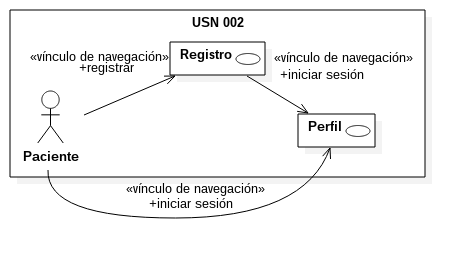
\includegraphics[width=1\textwidth]{figuras/usn/usn001_pac.png}
    \caption{USN-001}
    \label{fig:usn-001}
\end{figure}	

\begin{figure}[htbp] 
    \centering
    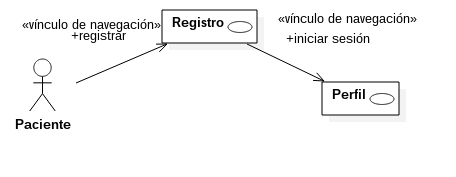
\includegraphics[width=1\textwidth]{figuras/usn/usn002_pac.png}
    \caption{USN-002}
    \label{fig:usn-002}
\end{figure}	

\begin{figure}[htbp] 
    \centering
    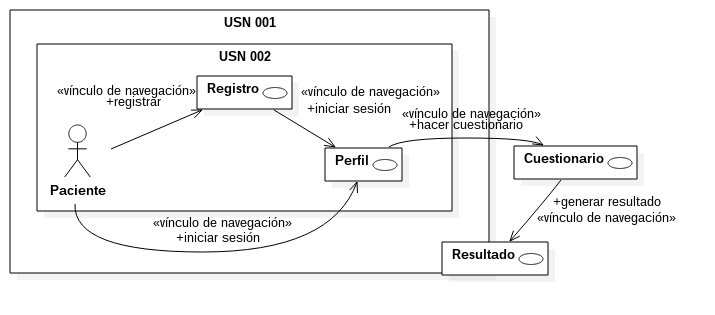
\includegraphics[width=1\textwidth]{figuras/usn/usn003.png}
    \caption{USN-003}
    \label{fig:usn-003}
\end{figure}	

\begin{figure}[htbp] 
    \centering
    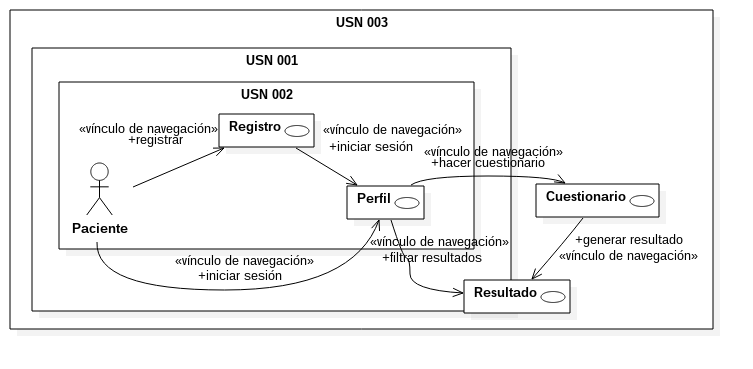
\includegraphics[width=1\textwidth]{figuras/usn/usn004.png}
    \caption{USN-004}
    \label{fig:usn-004}
\end{figure}	

\begin{figure}[htbp] 
    \centering
    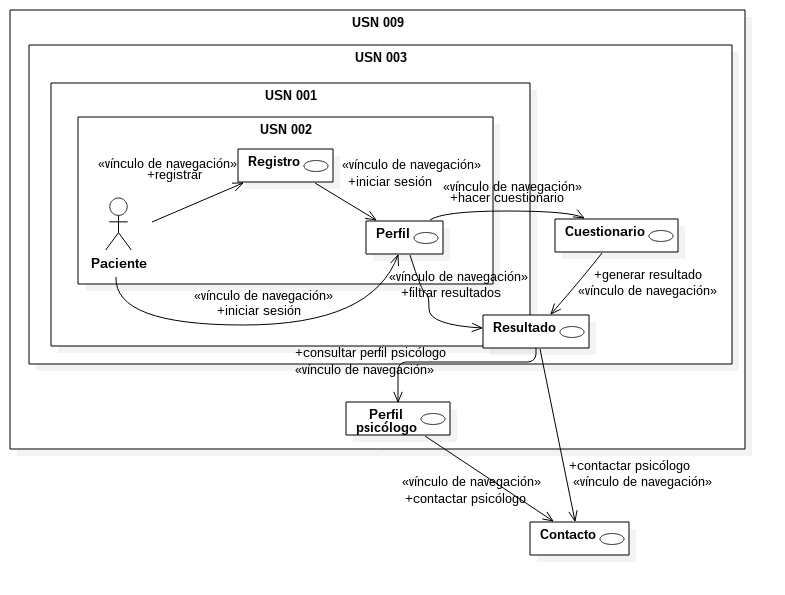
\includegraphics[width=1\textwidth]{figuras/usn/usn005.png}
    \caption{USN-005}
    \label{fig:usn-005}
\end{figure}	

\begin{figure}[htbp] 
    \centering
    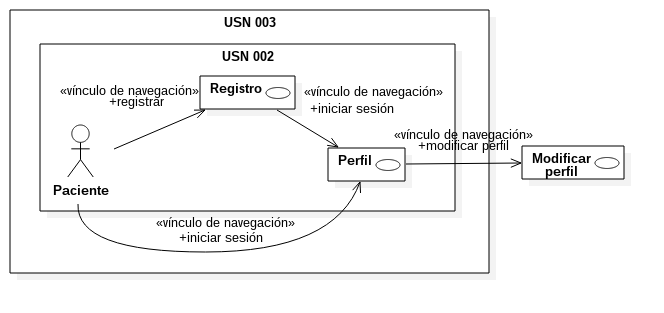
\includegraphics[width=1\textwidth]{figuras/usn/usn006.png}
    \caption{USN-006}
    \label{fig:usn-006}
\end{figure}	

\begin{figure}[htbp] 
    \centering
    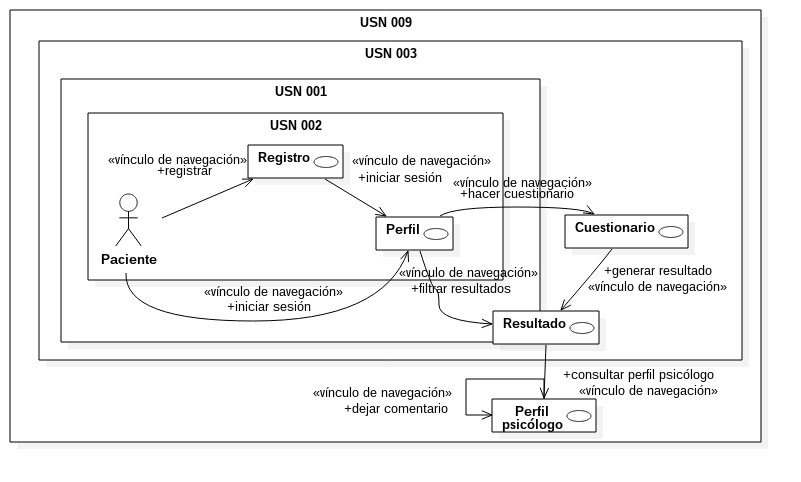
\includegraphics[width=1\textwidth]{figuras/usn/usn007.png}
    \caption{USN-007}
    \label{fig:usn-007}
\end{figure}	

\begin{figure}[htbp] 
    \centering
    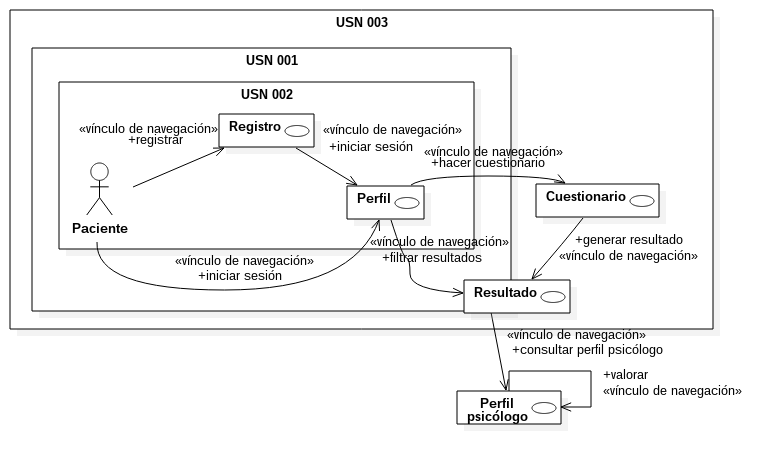
\includegraphics[width=1\textwidth]{figuras/usn/usn008.png}
    \caption{USN-008}
    \label{fig:usn-008}
\end{figure}	

\begin{figure}[htbp] 
    \centering
    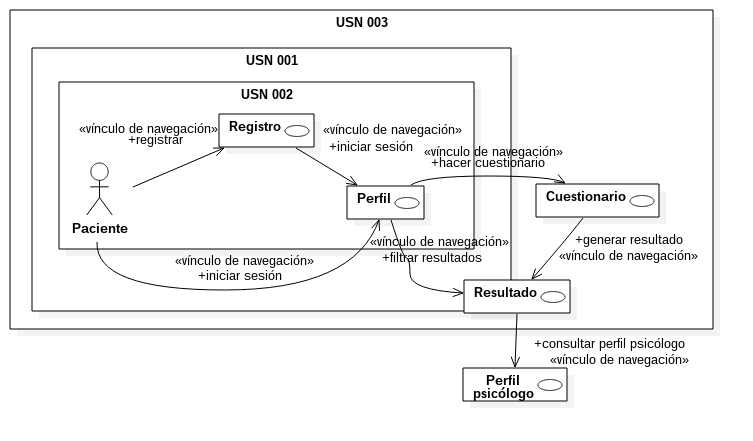
\includegraphics[width=1\textwidth]{figuras/usn/usn009.png}
    \caption{USN-009}
    \label{fig:usn-009}
\end{figure}	

\begin{figure}[htbp] 
    \centering
    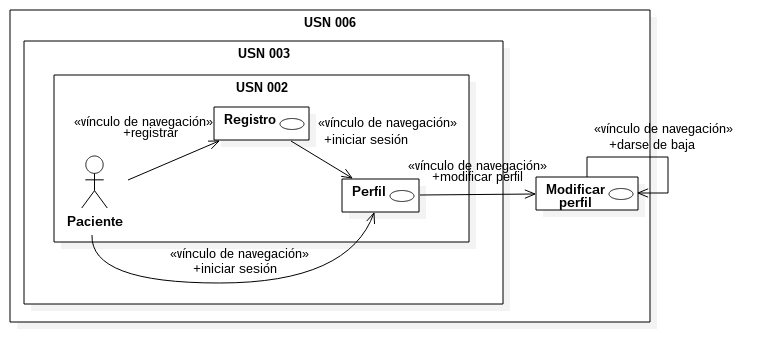
\includegraphics[width=1\textwidth]{figuras/usn/usn010.png}
    \caption{USN-010}
    \label{fig:usn-010}
\end{figure}	

\begin{figure}[htbp] 
    \centering
    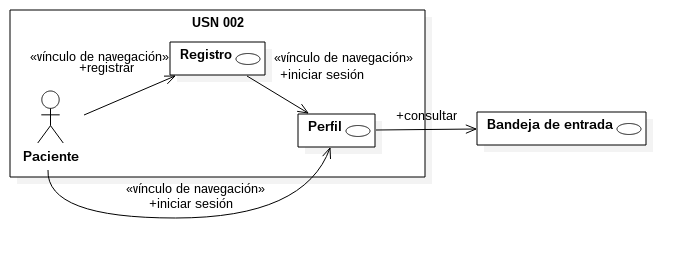
\includegraphics[width=1\textwidth]{figuras/usn/usn011_pac.png}
    \caption{USN-011 (Paciente)}
    \label{fig:usn-011-pac}
\end{figure}	

\begin{figure}[htbp] 
    \centering
    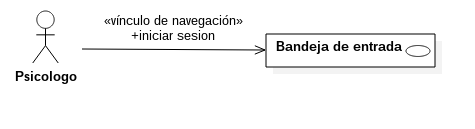
\includegraphics[width=1\textwidth]{figuras/usn/usn011_psic.png}
    \caption{USN-011 (Psicólogo)}
    \label{fig:usn-011-psic}
\end{figure}	

\begin{figure}[htbp] 
    \centering
    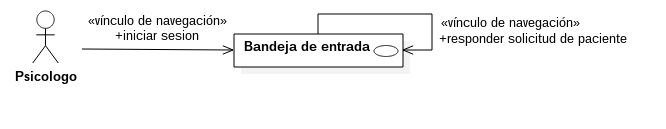
\includegraphics[width=1\textwidth]{figuras/usn/usn012.png}
    \caption{USN-012}
    \label{fig:usn-012}
\end{figure}	

\subsection{Sintaxis de navegación}
La sintaxis de navegación refleja la mecánica de la navegación para cada USN. Para nuestra plataforma web, se ha diseñado un mapa del sitio que describe todas las posibles navegaciones existentes. Para cada tipo de usuario (perfil o psicólogo), existe un mapa\ref{fig:map-nav} diferente.

\begin{figure}[htbp] 
    \centering
    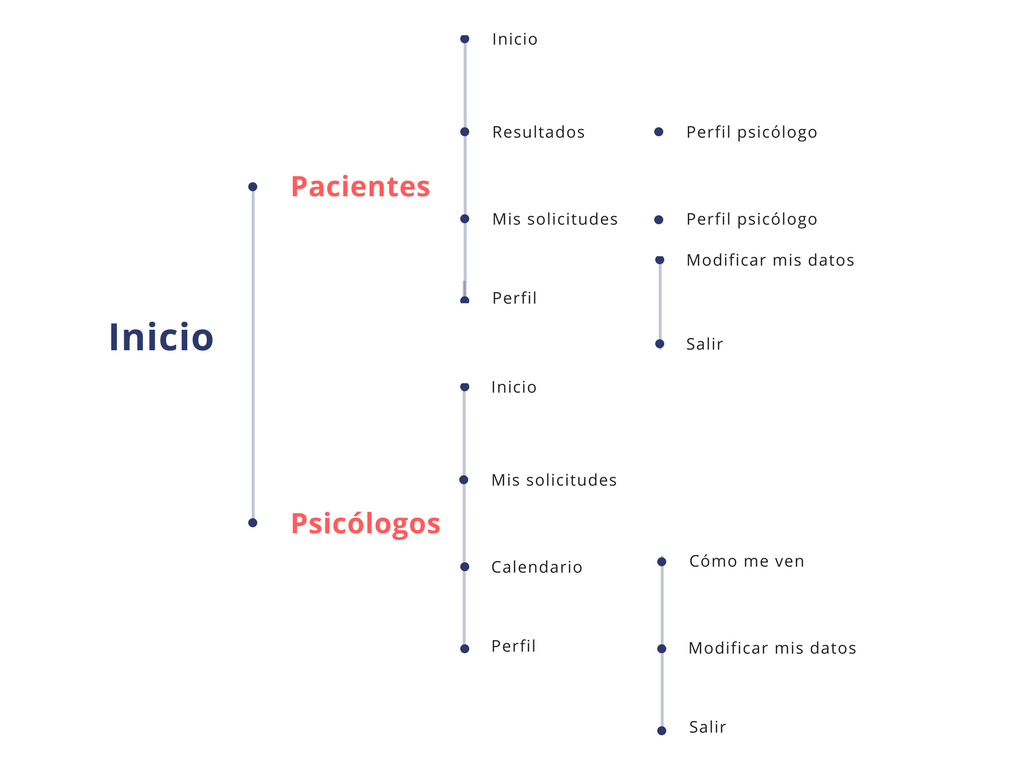
\includegraphics[width=1\textwidth]{figuras/Emozio_Mapa_Navegacion.png}
    \caption{Mapa de navegación}
    \label{fig:map-nav}
\end{figure}	

%%%%%%%%%%%%%%%%%%%%%%%%%%%%%%%%%%%%%%%%%%%%%%%%%%%%%%%%%%%%%%%%%%%%%%%%%%%%%%%%%%%%%%
%%%%%%%%%%%%%%%%%%%%%%%%%%%%%%%%%%%%%%%%%%%%%%%%%%%%%%%%%%%%%%%%%%%%%%%%%%%%%%%%%%%%%%
%TECNOLOGÍAS UTILIZADAS
%%%%%%%%%%%%%%%%%%%%%%%%%%%%%%%%%%%%%%%%%%%%%%%%%%%%%%%%%%%%%%%%%%%%%%%%%%%%%%%%%%%%%%
%%%%%%%%%%%%%%%%%%%%%%%%%%%%%%%%%%%%%%%%%%%%%%%%%%%%%%%%%%%%%%%%%%%%%%%%%%%%%%%%%%%%%%
\section{Tecnologías utilizadas}

\subsection{Frameworks}
Un \textit{framework} es una arquitectura de \textit{software} que modela las relaciones generales de las entidades del dominio, y provee una estructura y una especial metodología de trabajo, la cual extiende o utiliza las aplicaciones del dominio.


Los \textit{frameworks} involucrados en nuestro proyecto son MEAN Stack, Bootstrap y Semantic UI.


\subsubsection{MEAN Stack}
MEAN stack es un \textit{framework} para el desarrollo de aplicaciones, y páginas web dinámicas, basadas en JavaScript: MongoDB, ExpressJS, AngularJS y NodeJS, lo cual permite que se integren entre ellas eficazmente.


Con MongoDB podemos almacenar nuestros documentos en formato JSON, se pueden escribir consultas en nuestro servidor ExpressJS y NodeJS, y del mismo modo, pasar esos documentos JSON a nuestro \textit{frontend} hecho con AngularJS.


El \textit{debugging} y la administración de la base de datos se vuelven más sencillas cuando el objeto almacenado en la base de datos es idéntico al objeto que tu cliente JavaScript puede ver\cite{mongodb_mean_stack}.


Algunos de los motivos por los que escogí este \textit{framework} es por su escalabilidad, rapidez y flexibilidad, ya que permite que en un futuro sea sencillo poder adaptar la aplicación a plataformas móviles, o añadir cambios con facilidad.


Los componentes que forman el \textit{framework} son:


\begin{itemize}
\item \textbf{MongoDB}
MongoDB es una base de datos ágil NoSQL orientada a documentos que permite que los esquemas cambien rápidamente a medida que las aplicaciones evolucionan, proporcionando siempre la funcionalidad que los desarrolladores esperan de las bases de datos tradicionales, tales como índices secundarios, un lenguaje completo de búsquedas y consistencia. En resumen, MongoDB brinda escalabilidad, rendimiento y gran disponibilidad\cite{mongodb_gest_datos}. 
\item \textbf{ExpressJS}
ExpressJS es una middleware de aplicaciones web Node.js minimalista y flexible que proporciona un conjunto sólido de características para aplicaciones web y móviles\cite{express}. Se trata de una API REST que utiliza métodos HTTP para obtener datos o generar operaciones sobre esos datos.
\item \textbf{AngularJS}
AngularJS es un framework para construir client applications en HTML y Javascript, aunque también puede ser otro lenguaje como TypeScript que sea compilado a JavaScript. El framework posee un conjunto de librerías funcionales, y otras opcionales\cite{angular_docs}.


Angular permite fácilmente construir aplicaciones web, ya que combina declarative templates, dependency injection y end to end tooling, e integra buenas prácticas de programación. Las aplicaciones desarrolladas con Angular funcionan tanto para web, móvil o escritorio\cite{angular_arch}. 
\item \textbf{NodeJS}
NodeJS es un entorno de ejecución para JavaScript construido con el motor de JavaScript V8 de Chrome. Node.js usa un modelo de operaciones entrada/salida sin bloqueo (asíncrono) y orientado a eventos, que lo hace liviano y eficiente, ya que nunca se bloquea. 


Node está diseñado sin hilos, este presenta un bucle de eventos como un entorno en vez de una librería. Node simplemente ingresa el bucle de eventos después de ejecutar el script de entrada. Node sale del bucle de eventos cuando no hay más callbacks que ejecutar\cite{node_acerca}.
\end{itemize}


\subsubsection{Bootstrap}
Bootstrap es un \textit{framework} de código abierto para desarrollar con HTML, CSS y JS. Contiene características como un grid responsive, docenas de componentes, JavaScript plugins, tipografía, control de formularios y capacidad de personalización\cite{bootstrap}.


\subsubsection{Semantic UI}
Semantic UI es un \textit{framework} que permite a los desarrolladores contruir rápidamente sitios web, con HTML conciso, JavaScript intuitivo, y simplicando el \textit{debugging}. Semantic está diseñado de manera \textit{responsive} permitiendo que la aplicación sea escalable en múltiples dispositivos. Semantic está preparado para poder asociarse con otros frameworks como React, Angular, Meteor y Ember\cite{semantic_github}.


\subsection{Lenguajes de programación}
Los principales lenguajes de programación utilizados son:


\subsubsection{CSS3}
Hojas de Estilo en Cascada (Cascading Style Sheets) es el lenguaje utilizado para describir la presentación de documentos HTML o XML CSS describe como debe ser renderizado el elemento estructurado en pantalla, en papel, hablado o en otros medios\cite{css_mozilla}.


\subsubsection{HTML}
HTML, que significa Lenguaje de Marcado para Hipertextos (HyperText Markup Language) es el elemento de construcción más básico de una página web y se usa para crear y representar visualmente una página web. Determina el contenido de la página web, pero no su funcionalidad\cite{html_mozilla}.


\subsubsection{JavaScript}
Es un lenguaje ligero e interpretado, orientado a objetos con funciones de primera clase, más conocido como el lenguaje de script para páginas web, pero también usado en muchos entornos sin navegador, tales como node.js.


Es un lenguaje script multi-paradigma, basado en prototipos\footnote{La programación basada en prototipos es un estilo de programación orientada a objetos que reutiliza comportamientos de objetos existentes.}, dinámico, soporta estilos de programación funcional, orientada a objetos e imperativa\cite{javascript_mozilla}.


\subsection{	\textit{Modules}}
Un \textit{module} es cualquier fichero o directorio que puede ser cargado por NodeJS. 


\subsubsection{Mongoose}
Mongoose proporciona una sencilla, solución basa en esquemas para el modelo de los datos de la aplicación\cite{mongoose}.


\subsubsection{Bcrypt}
Bcrypt permite \textit{hashear} y comparar contraseñas en Node.


\subsubsection{NodeMailer}
NodeMailer permite a las aplicaciones el envío de mensajes.


\subsubsection{FullCalendar}
FullCalendar es un calendario de eventos JavaScript personalizable y de código abierto\cite{fullcalendar}.


\subsection{Librerías}
Una librería es un conjunto de implementaciones funcionales, codificadas en un lenguaje de programación, que ofrece una interfaz bien definida para la funcionalidad que se invoca.


\subsubsection{Places de Google Maps JavaScript API}
Las funciones de la biblioteca JavaScript de Google Places permite que una aplicación busque sitios (definidos en esta API como establecimientos, ubicaciones geográficas o puntos de interés destacados) dentro de un área definida, como los límites de un mapa o alrededor de un punto fijo. También, ofrece una función de autocompletado que puedes usar para dar a tus aplicaciones el comportamiento de escritura anticipada del campo de búsqueda de Google Maps. Cuando un usuario comienza a escribir una dirección, la función de autocompletado termina la tarea\cite{google_api}.


\subsection{	\textit{Middleware}}
Un \textit{middleware} proporciona la lógica de intercambio entre aplicaciones. El \textit{middleware} abstrae de la complejidad y heterogeneidad de las redes de comunicaciones subyacentes, así como de los sistemas operativos y lenguajes de programación, proporcionando una API para la fácil programación y manejo de aplicaciones distribuidas.


\subsubsection{Passport}
Passport es un \textit{middleware} de autenticación para NodeJS. Extremadamente flexible y modular. También puede ser utilizado en cualquier aplicación web basada en Express. Tiene múltiples estrategias que soportan autenticación utilizando nombre y contraseña, Facebook, Twitter, y más\cite{passport}. 


\section{Herramientas utilizadas}
Las herramientas utilizadas en este trabajo fueron:

\begin{itemize}
\item \textbf{Brackets}
\begin{itemize}
\item \textit{Descripción: }Brackets es un editor de texto de código abierto\cite{brackets}.
\item \textit{Uso: }Desarrollo software de la aplicación.
\end{itemize}
\item \textbf{Git}
\begin{itemize}
\item \textit{Descripción: }Git es un sistema de código abierto de control de versiones distribuído diseñado para manipular cualquier tipo de proyectos con rapidez y eficacia\cite{git}.
\item \textit{Uso: }Gestión de la configuración del proyecto.
\end{itemize}
\item \textbf{GitHub}
\begin{itemize}
\item \textit{Descripción: }Es una plataforma de desarrollo colaborativo que permite alojar proyectos utilizando el sistema de control de versiones de Git\cite{github}.  
\item \textit{Uso: }Gestión de la configuración del proyecto.
\end{itemize}
\item \textbf{Grunt}
\begin{itemize}
\item \textit{Descripción: }Es una herramienta que permite simplificar el proceso de construcción (build) de proyectos en JavaScript. Sirven para automatizar tareas repetitivas como minificación, compilación, testeo unitario...\cite{grunt}
\item \textit{Uso: }Durante el desarrollo de la aplicación.
\end{itemize}
\item \textbf{\LaTeX}
\begin{itemize}
\item \textit{Descripción: }Es un sistema tipográfico que incluye características diseñadas para la producción de documentación técnica y científica\cite{latex}.
\item \textit{Uso: }Elaboración de la memoria final.
\end{itemize}
\item \textbf{LibreOffice}
\begin{itemize}
\item \textit{Descripción: }Es un conjunto de aplicaciones de oficina: Writer, el procesador de textos, Calc, la hoja de cálculos, Impress, el editor de presentaciones, Draw, nuestra aplicación de dibujo y diagramas de flujo; entre otros\cite{libreoffice}. 
\item \textit{Uso: }Borradores y algunos diagramas del proyecto.
\end{itemize}
\item \textbf{Pencil}
\begin{itemize}
\item \textit{Descripción: }Pencil es una GUI de prototipado de código abierlo para creación de \textit{mockups}\cite{pencil}.
\item \textit{Uso: }Elaboración del \textit{mockup}.
\end{itemize}
\item \textbf{NPM}
\begin{itemize}
\item \textit{Descripción: }NPM es un gestor de paquetes JavaScript. Es el repositorio más grande de librerías de código abierto en el mundo\cite{npm}. 
\item \textit{Uso: }Instalación de paquetes y librerías software.
\end{itemize}
\item \textbf{Robomongo}
\begin{itemize}
\item \textit{Descripción: }Robomongo es una GUI que maneja la shell de MongoDB\cite{robomongo}.
\item \textit{Uso: }Gestión de la base de datos.
\end{itemize}
\item \textbf{StarUML}
\begin{itemize}
\item \textit{Descripción: }StarUML es una herramienta de modelado UML que permite hacer multitud de tipos de diagramas como de clase, de objeto, de casos de uso, de componente, entre otros\cite{staruml}. 
\item \textit{Uso: }Diseño de los diagramas del proyecto.
\end{itemize}
\end{itemize}

%%%%%%%%%%%%%%%%%%%%%%%%%%%%%%%%%%%%%%%%%%%%%%%%%%%%%%%%%%%%%%%%%%%%%%%%%%%%%%%%%%%%%%
%%%%%%%%%%%%%%%%%%%%%%%%%%%%%%%%%%%%%%%%%%%%%%%%%%%%%%%%%%%%%%%%%%%%%%%%%%%%%%%%%%%%%%
%SEGURIDAD
%%%%%%%%%%%%%%%%%%%%%%%%%%%%%%%%%%%%%%%%%%%%%%%%%%%%%%%%%%%%%%%%%%%%%%%%%%%%%%%%%%%%%%
%%%%%%%%%%%%%%%%%%%%%%%%%%%%%%%%%%%%%%%%%%%%%%%%%%%%%%%%%%%%%%%%%%%%%%%%%%%%%%%%%%%%%%
\section{Seguridad}
\subsection{¿Qué es Bcrypt?}
Niels Provos y David Maxieres diseñaron Bcrypt, una función de hashing de contraseñas basado en el tipo de cifrado Blowfish. Es empleado en algunas distribuciones de Linux por defecto. 


Cuando se genera un hash asociado a la contraseña por lo general los algoritmos comunes (md5, sha-1,…) incorporan un valor de salt, este fragmento se emplea para generar dicho hash, de esta forma se consigue que dos contraseñas iguales que generarían el mismo hash no lo hagan, algo muy importante para luchar contra ataques de fuerza bruta, así como para dificultar los ataques de Rainbow table.


Los ataque de Rainbow table son efectivos cuando las contraseñas son hasheadas de la misma manera, de esta forma para dos contraseñas iguales el hash sería el mismo. Así es como surge el salt, añadir un hash a cada contraseña nos devuelve dos hashes distintos para la misma contraseña. Es importante evitar la reutilización de salt. Sin embargo no es suficiente el uso de salt para el almacenamiento de contraseñas debido a que salt pasa a ser inútil para ataques de fuerza bruta o de diccionario.


\subsection{Ventajas de Bcrypt}
En este punto es donde entra Bcrypt, para solucionar el problema en el que nos hallamos debemos hablar del número de iteraciones. Esto mejora a los hashes comunes gracias a su lentitud. ¿Qué quiere decir esto? Empleando una variante de cifrado Blowfish se introduce un factor de trabajo que permite controlar el coste de la función hash. Mediante este factor Bcrypt se actualiza de acuerdo a la ley de Moore con la evolución de la tecnología.


Para verlo más concretamente podemos ver la tabla de comparación siguiente, y recalcar que aunque las contraseñas no requieran de una protección tan elevada, gracias al factor de trabajo la optimización de bcrypt se consigue con un buen equilibrio entre velocidad y seguridad. El sacrificio de un poco de rendimiento se traduce en un aumento de la seguridad. 
Esta tabla muestra una prueba de la fuerza de bcrypt, que ha sido lanzado en un clúster de 25 GPU para la rotura de contraseñas en hash, han resultado los siguientes datos:


\begin{itemize}
\item md5(\$password) 
\begin{itemize}
\item 180 billones resultados/s
\item 9.4 Horas
\end{itemize}
\item sha1(\$password)
\begin{itemize}
\item 61 billones resultados/s
\item 27 Horas
\end{itemize}
\item md5crypt
\begin{itemize}
\item 77 millones resultados/s
\item 2.5 Años
\end{itemize}
\item bcrypt con un factor de 5 
\begin{itemize}
\item 71 mil resultados/s
\item 2700 Años
\end{itemize}
\end{itemize}


\subsection{Funcionamiento}
La librería bcrypt nos permite crear el hash de una contraseña mediante saltRounds, este valor nos da control sobre el factor de coste de procesado de datos. A mayor valor de SaltRound mayor coste de cálculo del hash asociado a una contraseña.  Por defecto este valor viene situado en 10. 


En el caso del registro de usuario se envía la contraseña y el valor del parámetro SaltRounds a la librería para que la cifre, esta nos devuelve el hash asociado a la contraseña en el usuario de la base de datos. Cuando el usuario quiere entrar la contraseña introducida se cifra, para ello se busca el salt asociado al usuario de la base de datos. Una vez cifrada con el salt se comparan los hashes. La librería nos devuelve un booleano que indica si las contraseñas coinciden o no, con lo cual podemos dejar entrar el usuario o devolver un error.


\subsection{Cifrado Blowfish}
Bruce Schneier en 1993 diseña un codificador de bloques simétricos de 64 bits, con claves de hasta 448 bits, es empleado en un abundante número de productos de cifrado. No tiene técnicas de criptoanálisis que hayan resultado efectivas contra este algoritmo. Su licencia es totalmente libre.


%%%%%%%%%%%%%%%%%%%%%%%%%%%%%%%%%%%%%%%%%%%%%%%%%%%%%%%%%%%%%%%%%%%%%%%%%%%%%%%%%%%%%%
%%%%%%%%%%%%%%%%%%%%%%%%%%%%%%%%%%%%%%%%%%%%%%%%%%%%%%%%%%%%%%%%%%%%%%%%%%%%%%%%%%%%%%
%DISEÑO DE LA ARQUITECTURA
%%%%%%%%%%%%%%%%%%%%%%%%%%%%%%%%%%%%%%%%%%%%%%%%%%%%%%%%%%%%%%%%%%%%%%%%%%%%%%%%%%%%%%
%%%%%%%%%%%%%%%%%%%%%%%%%%%%%%%%%%%%%%%%%%%%%%%%%%%%%%%%%%%%%%%%%%%%%%%%%%%%%%%%%%%%%%
\section{Diseño de la arquitectura}

\subsection{SPA}
\textit{Single page aplication}, de ahora en adelante SPA, es una aplicación o sitio web que cabe en una sóla página web con el objeto de proveer una experiencia de usuario más fluída y una interfaz más enriquecida. Una de las ventajas de este tipo de aplicaciones es que son capaces de actualizar una parte de la interfaz, sin necesidad de enviar o recibir una petición de full-page.


\subsection{Particularidades de JavaScript}
\subsubsection{En JavaSCript no existen las clases}
JavaScript es un lenguaje orientado a objetos basado en prototipos en lugar de clases. A diferencia de los lenguajes orientados a objetos basados en clases, un lenguaje basado en prototipos no hace distinción entre clases e instancias: Simplemente tiene objetos. Estos objetos son conocidos como objetos prototípicos, que son objetos que se utilizan como una plantilla a partir de la cual se obtiene el conjunto inicial de propiedades de un nuevo objeto\cite{fernandomonteiro2014}.


Para poder entender cuáles son las diferencias entre un lenguaje orientado a objetos basados en clases (Java) y basados en prototipos (JavaScript) se han listado sus diferencias en la tabla \ref{java-js}.


\begin{table}[htpb]
\centering
\begin{tabular}{|l|l|}
\hline
\textbf{Basados en clases (Java)}                                                                                                                                       & \textbf{Basados en prototipos (JavaScript)}                                                                                                                                                  \\ \hline
La clase y su instancia son entidades distintas                                                                                                                         & Todos los objetos pueden heredar de otro objeto                                                                                                                                              \\ \hline
Define una clase en la definición de clase; se instancia una clase con los métodos constructores.                                                                       & Define y crea un conjunto de objetos con funciones constructoras.                                                                                                                            \\ \hline
Se crea un objeto con el operador new.                                                                                                                                  & Igual.                                                                                                                                                                                       \\ \hline
Se construye una jerarquía de objetos utilizando la definición de las clases para definir subclases de clases existentes.                                               & Se construye una jerarquía de objetos mediante la asignación de un objeto como el prototipo asociado a una función constructor.                                                              \\ \hline
Se heredan propiedades siguiendo la cadena de clases.                                                                                                                   & Se heredan propiedades siguiendo la cadena de prototipos.                                                                                                                                    \\ \hline
La definición de una clase especifica todas las propiedades de todas las instancias de esa clase. No se pueden añadir propiedades dinámicamente en tiempo de ejecución. & El conjunto inicial de propiedades lo determina la función constructor o el prototipo. Se pueden añadir y quitar propiedades dinámicamente a objetos específicos o a un conjunto de objetos. \\ \hline
\end{tabular}
\caption{Comparativa Java y JavaScript}
\label{java-js}
\end{table}


Por estos motivos, los patrones que se han diseñado con UML consisten en una aproximación de cómo se representaría el diseño de la plataforma.


\subsection{	\textit{Callbacks} en JavaScript}
Las \textit{callbacks} JavaScript son utilizadas para gestionar eventos de manera responsable en el lado cliente ejecutando funciones asíncronas, y en Node, las \textit{callbacks} también son utilizadas en el lado servidor para dar servicio a múltiples peticiones simultáneas de clientes.


Una \textit{callback} es una función que es pasada como argumento a otra función, que espera ser invocada tanto inmediátamente como en algún momento futuro.


Las \textit{callbacks} pueden ser vistas como una forma de ``\textit{continuation-passing style}'' (CPS), cuyo control es pasado explícitamente de forma continuada, en el caso de las \textit{callback} es pasado como argumento representando una continuación.


JavaScript utiliza un modelo \textit{event-driven} con un único hilo de ejecución. Programar con \textit{callbacks} es especialmente útil cuando el llamador no quiere esperar hasta que la llamada se complete. Para conseguirlo, la operación no bloqueante (\textit{non-blocking operation}) es agendada (\textit{scheduled}) como una \textit{callback} y el hilo principal continua su síncrona ejecución. Cuando la operación se completa, un mensaje es encolado en una cola de tareas según la \textit{callback} que lo provee. El bucle de eventos (event loop) en JavaScript prioriza que el hilo ejecute la pila de llamadas primero; cuando la pila está vacía, el bucle de eventos desencola un mensaje para la cola de tareas y ejecuta la correspondiente función \textit{callback}.
En JavaScript, las \textit{callbacks} pueden llamarse “funciones” o “funciones anónimas”.
En el proyecto, para gestionar las \textit{callbacks} se han utilizado promises. Las \textit{promise} son una extensión del lenguaje JavaScript \cite{keheliyagallabaalimesbahivanbeschastnikh2015}.


Una \textit{promise} es un \textit{proxy} para un valor no necesariamente conocido en el momento que es creada. Permite asociar manejadores que actuarán asincrónicamente sobre un eventual valor en caso de éxito, o la razón del fallo. Esto permite que métodos asíncronos devuelvan valores como si fueran síncronos: en vez de inmediatamente retornar el valor final, el método asíncrono devuelve una \textit{promise} y suministra su valor en algún momento en el futuro\cite{promise_objeto}. Al objeto le enganchas las funciones \textit{callback}, en vez de pasar funciones \textit{callback} a una función\cite{promise_mozilla}. Nos permiten mejorar la legibilidad de nuestro código y evitar tener que pasar el contenido de las funciones directamente como argumentos a nuestra llamada. Las \textit{promise} en JavaScript sirven para evitar el ``\textit{callback-hell}''que surge de llamar a una función asíncrona en JavaScript. 


\subsubsection{Implementando patrones de diseño con JavaScript}
En la mayoría de lenguajes tradicionales orientados a objetos existen las clases, las interfaces, la herencia, la encapsulación y el polimorfismo. Pero JavaScript, no, puesto que es muy sencillo: Trabaja por medio de callbacks (funciones).


Un objeto es la unidad responsable de proporcionar estados y comportamiento; y la declaración de las funciones en JavaScript proporcionan ambas\cite{angular_embraced}.


\subsection{Patrones de diseño}
\subsubsection{MVC y MVVM}
El patrón Modelo Vista Controlador, de ahora en adelante MVC, es un patrón de arquitectura software que permite separar la representación visual de la información, de la interacción del usuario. 


MVC es un patrón \textit{composite}. Los patrones \textit{composite} son aquellos patrones capaces de trabajar juntos para darle solución a un problema en común\cite{ericfreemanelisabethfreemankathysierrabertbates2004}. 


El patrón de diseño MVC está compuesto por:


\begin{itemize}
\item Modelo: Almacena toda la información, estados y lógica de la aplicación.
\item Vista: Se trata de a interfaz de usuario que muestra una representación del modelo. La vista informa al controlador qué trata de hacer el usuario. 
\item Controlador: Toma la entrada del usuario, la gestiona y le transmite lo que ha interpretado al modelo. También, manipula cómo se debe ver la vista.
\end{itemize}


Actualmente, se han desarrollado nuevos tipos de modelo MV*, como el Modelo Vista VistaModelo, de ahora en adelante MVVM, que está basada en el patrón MVC y el Modelo Vista Presentador, que trata de separar con más claridad el desarrollo de la interfaz de usuario con el de la lógica de negocio y el comportamiento de la aplicación.


Los componentes de los patrones MVVM son:


\begin{itemize}
\item Modelo: Representa los datos específicos del dominio o información con la que nuestra aplicación debe trabajar. Almacena información, pero comunmente no posee ningún tipo de comportamiento. No formatean la información ni influencian en cómo los datos aparecen en el navegador, ya que no es su responsabilidad.
\item Vista: Es la única parte de la aplicación con la que el usuario interactúa. Contiene la información obtenida de la sincronización entre la vista y el modelo (\textit{data binding}\cite{data_binding_w3s}), los eventos y comportamientos. Es una interfaz de usuario interactiva que representa el estado de la VistaModelo. La vista no es la encargada de gestionar su estado, sólo se mantiene sincronizada con la VistaModelo.
\item VistaModelo: Se puede considerar como un Controlador especializado que actúa como un conversor de datos. Transforma la información del Modelo en la información de la Vista\cite{fernandomonteiro2014}. 
\end{itemize}

En MEAN STACK, estos dos patrones se pueden aparecen combinados como se muestra en la figura\ref{fig:mvc_mvvm}.


\begin{figure}[htbp] 
    \centering
    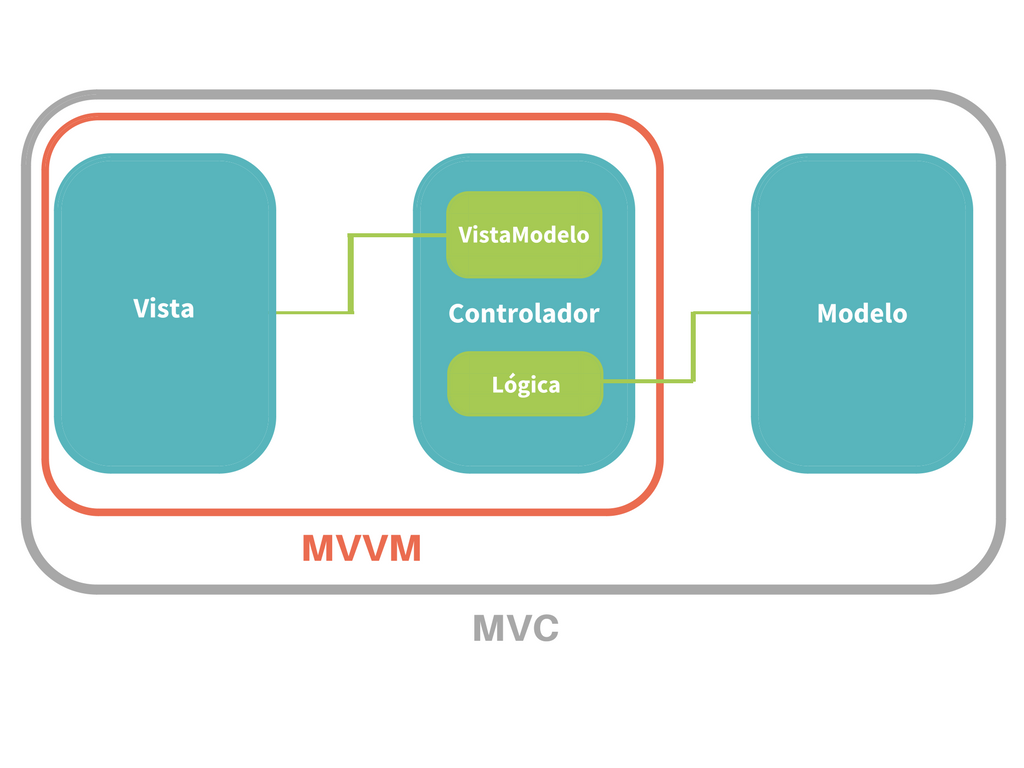
\includegraphics[width=1\textwidth]{figuras/MVC_MVVM.png}
    \caption{Mean STACK - MVC y MVVM}
    \label{fig:mvc_mvvm}
\end{figure}	


\subsubsection{\textit{Page Controller}}
\textit{Page Controller} tiene un único \textit{controller} por cada página lógica de la página web\cite{martinfowlerdavidricematthewfoemmeledwardhieattrobertmeerandystafford2002}.


Las responsabilidades del \textit{Page Controller} son:


\begin{itemize}
\item Analizar la URL y extraer cualquier dato de formulario necesario para el comportamiento.
\item Crear e invocar cualquier objeto del modelo para procesar datos. Cualquier dato relevante de una petición HTML ha de ser pasada al modelo, de esta forma el modelo no necesita ningún tipo de conexión a las peticiones HTML.
\item Determina qué vista ha de ser mostrada a continuación como resultado de la página y proporcionar al modelo información sobre ello.
\end{itemize}


El patrón \textit{Page Controller} acepta entradas desde la petición de una página, invoca las acciones pedidas en el modelo, y determina la vista que se ha de usar como página resultante\cite{page_controller_microsoft}.


En AngularJS, tenemos \textit{controllers} los cuales tienen unas responsabilidades limitadas: Ellos no aceptan las peticiones del usuario porque es la responsabilidad de los \textit{services} \$route o \$state y la renderización de la página es responsabilidad de la directiva ng-view. Para determinar qué vista ha de ser mostrada utiliza el \textit{service} \$location.


Al igual que \textit{page controllers}, los \textit{controllers} de AngularJS gestionan las interacciones de usuario, proveen y actualizan los modelos. El modelo está unido a la vista a través de \$scope\cite{mgechev}.


\subsection{	\textit{Observer}}
El patrón \textit{Observer} es un patrón de diseño \textit{software} en el cual un objeto, llamado \textit{subject}, mantiene una lista de sus dependencias, llamadas \textit{observers}, y las notifica automáticamente en cualquier cambio de estado, normalmente utilizando uno de sus métodos. 


\subsubsection{\textit{Data-binding}}
\textit{Data binding} en Angular es la sincronización entre el modelo y la vista.


El \textit{controller} proporciona comportamiento a través de \$scope, mientras que {{}} se pueden utilizar en el código HTML para mostrar contenido del modelo en la vista. O la \textit{directive} ng-model para asociar el modelo con la vista.


Cuando la información en el modelo cambia, la vista refleja dicho cambio, y cuando la vista es modificada, el modelo se actualiza.


Debida a la inmediata sincronización entre el modelo y la vista, el controlador puede estar completamente separado de la vista, y simplemente concentrarse en el modelo de datos\cite{data_binding_w3s}.


El mostrado en la figura \ref{fig:data_binding} representa el funcionamiento descrito a continuación. El \textit{module} es el objeto de mayor nivel en Angular. Una aplicación Angular es especificada por la directiva ng-app siempre correspondiente a un módulo.
Config es un objeto que configura la aplicación Angular, permite configurar las rutas (\textit{routes}) necesarias en la SPA porque gestionan las \textit{templates}. En Angular se empareja cada \textit{template} con un \textit{controller}. La <view> representa la parte \textit{front-end} y el \textit{controller} y la \textit{factory}  representan el \textit{back-end}. \$scope vive entre ambos, y Angular permite asegurar que ambos tengan la última versión de la aplicación. El bucle de eventos y \$scope permiten a Angular \textit{two way data binding}, y como resultado es que ya no es necesario acceder al DOM desde JavaScript\cite{praislee}.   


\begin{figure}[htbp] 
    \centering
    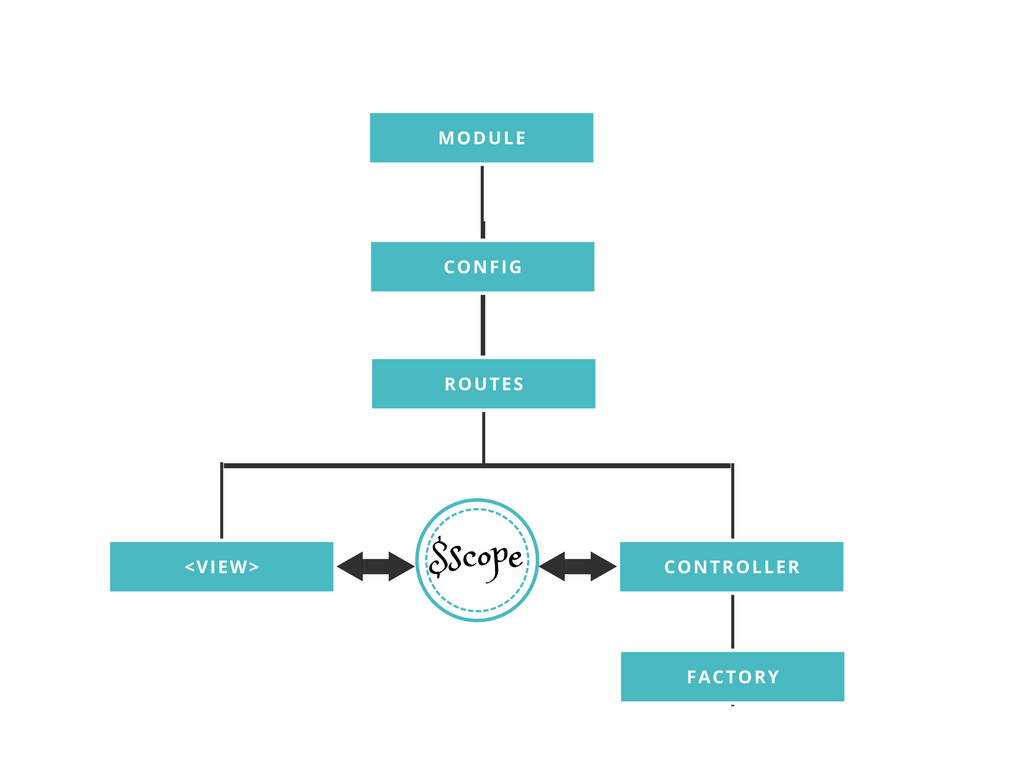
\includegraphics[width=1\textwidth]{figuras/data_binding.png}
    \caption{Esquema \textit{data-binding}}
    \label{fig:data_binding}
\end{figure}	


\subsubsection{\textit{Dependency Injection}}
\textit{Dependency injection} permite obtener una instancia de las clases que se requieren y que una \textit{factory} o \textit{injector} te las provea tanto en tiempo de compilación como en el de ejecución\cite{depend_inject}.


\textit{Dependency injection} suele ser utilizado para evitar al patrón \textit{Singleton}\cite{mgechev}.


\subsection{\textit{Factory Method}}
Los propósitos del patrón \textit{Factory} son:


\begin{itemize}
\item Crear objetos
\item Realiza operaciones repetitivas cuando se preparan objetos similares.
\item Ofrece que los consumidores de la \textit{Factory} puedan crear objetos sin necesidad de conocer el tipo específico (de la clase) en tiempo de compilación\cite{stoyanstefanov2010}.
\end{itemize}


El patrón \textit{factory} provee una interfaz genérica para crear objetos, donde hay que especificar el tipo de objeto \textit{factory} que deseamos obtener\cite{addyosmani2012}.


En AngularJS se hace por medio del \textit{Factory Method}\cite{mgechev}.


\subsection{	\textit{Proxy}}
En el patrón \textit{proxy}, un objeto actúa como interfaz de otro objeto. El \textit{proxy} se encuentra entre el cliente de un objeto y el objeto en sí, protegiendo el acceso a dicho objeto.


Al tratarse de un \textit{proxy} virtual solventa la problemática que existe si inicializar el sujeto real es costoso, y puede ocurrir que el cliente lo inicialice pero nunca llegue a usarlo. En este caso, el \textit{proxy} puede ayudar siendo la interfaz del sujeto real. El \textit{proxy} recibe la petición de inicialización, pero nunca lo pasa a no ser que realmente el sujeto real sea utilizado. 


La imagen \ref{fig:proxy}, muestra el posible escenario de cuando un cliente realiza una petición de inicialización y el \textit{proxy} responde que todo está bien, pero realmente no pasa el mensaje, a no ser que sea obvio que el cliente necesite hacer algo con el sujeto. Sólo en ese caso, el \textit{proxy} le pasará ambos mensajes juntos\cite{stoyanstefanov2010}.
 

\begin{figure}[htbp] 
    \centering
    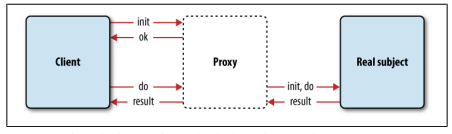
\includegraphics[width=1\textwidth]{figuras/proxy_pattern.png}
    \caption{\textit{Proxy pattern}\cite{stoyanstefanov2010}}
    \label{fig:proxy}
\end{figure}	


\subsection{\textit{Data Mapper}}
Un \textit{Data Mapper} es una capa de acceso a datos (\textit{Data Access Layer}) que permite la transferencia bidireccional de datos entre el lugar de almacenamiento de los datos persistentes y la representación en memoria de esos datos, manteniéndolos independientes\cite{mgechev}.


En Angular a través del módulo ngResource, nos permite realizar conexiones REST a nuestra API para enviar y recibir información mediante el servicio \$http. Sin embargo, los datos pasados desde el servidor se encuentran en un formato apropiado gracias a la librería Mongoose.


Mongoose proporciona por un lado el esquema que da formato a los datos obtenidos de la base de datos, y por otro lado, el acceso a los mismos. 


\subsection{API REST}
REST (\textit{Representational State Transfer}) es un estilo de arquitectura diseñado para sistemas distribuídos. No está estandarizado pero posee una serie de directivas, como permanecer sin estado, tener relaciones cliente-servidor y una interfaz uniforme. Suele estar relacionado con HTTP.


Sus principios son:


\begin{itemize}
\item Expone recursos fácilmente con un directorio de URLs estructurado.
\item Representa los data objects y atributos en formato JSON o XML.
\item Los mensajes utilizan métodos HTTP explícitamente: GET, POST, PUT y DELETE.
\item Protocolo cliente/servidor sin estado: Cada petición HTTP contiene toda la información necesaria para ejecutarla, lo que permite que ni cliente ni servidor necesiten recordar ningún estado previo para satisfacerla\cite{rest_spring}.
\end{itemize}


\subsection{Estructura de directorios}
Es importante mantener una estructura de directorios\ref{fig:directorios} y de código organizada, pensando en el mantenimiento y en la escalabilidad de la aplicación. 


A continuación, se describen (por orden de aparición) los distintos directorios y ficheros que pertenecen a la estructura básica del proyecto:


\begin{itemize}
\item app
Contiene la parte frontend de la aplicación.
\item assets
Contiene algunos de los recursos de la aplicación.
\item images
Contiene las imágenes utilizadas en la aplicación.
\item javascript
Contiene todos los archivos JavaScript de la parte frontend de la aplicación.
\item app.js
Es nuestro fichero de inicio.
\item controllers
Contiene los controllers de los templates.
\item routes.js
Archivo que determina el enrutado de nuestra aplicación.
\item factories
Contiene los factories.
\item vendor
Contiene algunas librerías JavaScript utilizadas en la aplicación.
\item semantic
Contiene todos los archivos del paquete semantic-ui.
\item styles
Contiene algunas librerías CSS utilizadas en la aplicación.
\item templates
Contiene los templates de la aplicación.
\item views
Contiene la view de nuestra aplicación.
\item app.js
Archivo de configuración del arranque del servidor.
\item node\_modules
Contiene todos los paquetes Node.js utilizados en la aplicación.
\item npm-shrinkwrap.json
Archivo que mantiene un registro de versiones de los paquetes. 
\item package.json
Archivo que mantiene una lista de los paquetes de los que depende la aplicación.
\item README.md
Archivo que describe brevemente la aplicación.
\item semantic.json
Archivo que contiene configuraciones de compilación para Gulp.
\item server
Contiene la parte backend de la aplicación.
\item config
Contiene ficheros de configuración de la aplicación.
\item expressConfig.js
Archivo que contiene configuración de Express.js.
\item models
Contiene los models de la aplicación.
\item routes
Contiene las rutas API REST de la aplicación.
\item routes.js
Archivo que configura los módulos y enrutamiento de la aplicación.
\end{itemize}


\begin{figure}[htbp] 
    \centering
    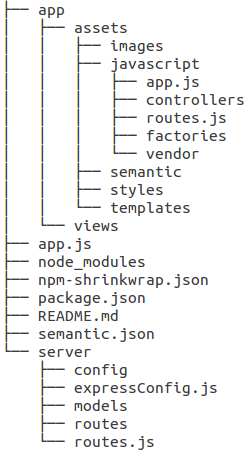
\includegraphics[width=0.5\textwidth]{figuras/directorios.png}
    \caption{Estructura de directorios}
    \label{fig:directorios}
\end{figure}	

\section{Diagramas}


%\cleardoublepage
%IMPLEMENTACIÓN
\chapter{Implementación}

En las secciones siguientes se mencionarán los aspectos más relevantes de la implementación.\newline

\section{Implementación del primer incremento}
El primer incremento fue la primera toma de contacto con la tecnología utilizada tras la formación.\newline



Los requisitos implementados en el primer incremento son los asociados a la parte del cuestionario de emparejamiento:



\begin{itemize}
\item RF-005: Emparejamiento 
\item RF-006: Filtrado de los resultados en base a distintos criterios
\item RNF-002: Tiempo de respuesta de asignación
\end{itemize}



Las tareas más trascendentales realizadas en este incremento son las descritas a continuación:


 
\paragraph*{Configuración Angular}
Todos los archivos Angular utilizados deben importarse en la \textit{root view} (app/views/index.html en el proyecto): Librerías JavaScript, app.js, route.js, controllers y factories.\newline



Para indicar a la aplicación que se trata de una aplicación Angular se debe especificar en la etiqueta <html> de la \textit{root view} (app/views/index.html) de la siguiente forma:



\medskip
\begin{lstlisting}
<html ng-app="Emozio"> </html>
\end{lstlisting}



Se define el módulo principal de la aplicación en el archivo app/assets/javascript/app.js:



\medskip
\begin{lstlisting}
angular.module('Emozio', ['ngRoute', 'ngResource']);
\end{lstlisting}



Entre corchetes se encuentran las dependencias que tiene nuestro módulo Emozio:



\begin{itemize}
\item \texttt{ngRoute}: Permite a la aplicación convertirse en una SPA, permitiendo la navegación ente distintas páginas sin necesidad de recargar. W3 angular-routing
\item \texttt{ngResource}: Permite crear objetos para interactuar con los datos RESTful del lado servidor. El objeto devuelto tiene métodos de acción que proporcionan comportamiento sin necesidad de interactuar con el servicio \$http a bajo nivel. Las acciones por defecto son:
\end{itemize}


\medskip
\begin{lstlisting}
{ 'get':    {method:'GET'}, 
  'save':   {method:'POST'}, 
  'query':  {method:'GET', isArray:true}, 
  'remove': {method:'DELETE'}, 
  'delete': {method:'DELETE'} };
\end{lstlisting}



Llamar a estos métodos invoca a \$http con el método http especificado, destino y parámetros.



Para indicar al \$routeProvider dónde mostrar las templates se utiliza la siguiente directiva: \texttt{<div ui-view></div>}


 
\paragraph*{Implementación de las \textit{templates} y \textit{controllers} de los requisitos. Éstos se encuentran dentro del directorio app/assets.}



\begin{table}[H]
\centering
\begin{tabular}{|l|l|}
\hline
\rowcolor[gray]{0.9}\textit{\textbf{Template}}           & \textit{\textbf{Controller}}        \\ \hline
pacientes/cuestionarioPacientes.html & pacientes/cuestionarioController.js \\ \hline
pacientes/pacientesResultados.html   & pacientes/perfilController.js       \\ \hline
\end{tabular}
%\caption{My caption}
%\label{my-label}
\end{table}


 
\paragraph*{Creación de las \textit{factories}, \textit{routes} y \textit{models} de: Paciente, Psicologo y Patologia.}


 
\paragraph*{Configuración de la conexión con la BBDD en un archivo aparte: server/config/dbConnection.js}



\medskip
\begin{lstlisting}
var MONGO_URL = 'mongodb://localhost:27017/emozio';
\end{lstlisting}




Se define la URL de la base de datos a la que se conecta la app.



\medskip
\begin{lstlisting}
	var options = {
		useMongoClient: true,
		autoIndex: false, // No crear index
		reconnectTries: Number.MAX_VALUE, // Nunca para de reintentar conectarse
		reconnectInterval: 500, // Reconexion cada 500ms
		poolSize: 10, // Mantener una conexion de 10 sockets
		// Si no se conecta, devuelve un error inmediatamente antes de tratar de reconectarse
		bufferMaxEntries: 0
	};
\end{lstlisting}



Se establecen las opciones de conexión.



\medskip
\begin{lstlisting}
mongoose.Promise = global.Promise;
\end{lstlisting}



Se declara que las \textit{promise} que va a utilizar Mongoose son las globales proporcionadas por Bluebird. En la base de datos utilizamos las \textit{promise} definidas e implementadas en la librería Bluebird.



\medskip
\begin{lstlisting}
mongoose.connect(MONGO_URL, options, function(err, res) {
	if(err) {
		console.log('ERROR: Reconectando a la BBDD. ' + err);
	}else{
		console.log("Conectado a la BBDD");
	}
});
\end{lstlisting}



Función de conexión de Mongoose a la base de datos con las opciones especificadas.



\medskip
\begin{lstlisting}
	var db = mongoose.connection;
	/* Si sucede un error, mostrarlo */
	db.on('error', console.error.bind(console, 'Error de conexion:'));
	db.once('open', function() {
		console.log("Con exito");
	});
\end{lstlisting}



Se abren las conexiones a la base de datos.


 
\paragraph*{Configuración ExpressJS en server/expressConfig.js}


\medskip
\begin{lstlisting}
app.use("/", express.static("app/"));
\end{lstlisting}


Con express.static se especifican los directorios donde se encuentran los archivos que Express va a leer. Facilita el acceso a los \textit{assets} (bienes) de la carpeta app desde el servidor. Lo que nos permite tener la parte cliente separada del servidor. 


\medskip
\begin{lstlisting}
app.set('views', __dirname + '/../app/views');
\end{lstlisting}


Define que las routes a las templates se rendericen con el render method dentro del directorio views.


\medskip
\begin{lstlisting}
app.use(bodyParser.urlencoded({ extended: true }));
\end{lstlisting}


Especifica que los datos recogidos de un formulario se pasen a través del método \textit{post}.


\medskip
\begin{lstlisting}
app.use(bodyParser.json());
\end{lstlisting}


Mediante el paquete Body-parser, podemos tratar los objetos en formato JSON sin necesidad de manipularlos, o cambiar su tipo.

 
\paragraph*{Especificación del arranque del servidor y se establece cuál es la vista raíz en el archivo routes.js. También, se vinculan todos los archivos que va utilizar el servidor: Archivos de configuración, de conexiones al modelo...}


\medskip
\begin{lstlisting}
var app = express();
\end{lstlisting}


Se inicializa el servidor express.


\medskip
\begin{lstlisting}
	app.get('/', function(req, res){
		res.sendfile('index.html', {root: app.settings.views});
	});
\end{lstlisting}


Express establece cuál va a ser la \textit{view} raíz (\textit{root}) enviada tras el inicio del servidor.


Además, se importan los archivos de server/routes que sirven como \textit{endpoint} (punto medio) entre la parte cliente y servidor, de esta forma durante la implementación, logramos mantener la parte del \textit{frontend} independiente del \textit{backend} haciéndola funcional.


\section{Implementación del segundo incremento}
Los requisitos implementados en el segundo incremento son los asociados a la parte de la gestión de usuarios:


\begin{itemize}
\item RF-001: Acceso usuarios
\item RF-002: Registro
\item RF-003: Baja
\item RF-004: Modificación de los datos
\item RNF-001: Encriptado de datos
\end{itemize}


\begin{table}[H]
\centering
\begin{tabular}{|l|l|}
\hline
\rowcolor[gray]{0.9}\textit{\textbf{Template}}           & \textit{\textbf{Controller}}        \\ \hline
inicio.html & pacientes/pacientesAccesoController.js \\ \hline
pacientes/registroPacientes.html   & pacientes/pacientesRegistroController.js       \\ \hline
pacientes/pacientesModificar.html   & pacientes/pacientesModificarController.js
       \\ \hline
psicologos/psicologosModificar.html      & psicologos/psicologosModificarController.js       \\ \hline
psicologos/registroPsicologo.html         & psicologos/psicologosRegistroController.js
       \\ \hline
\end{tabular}
%\caption{My caption}
%\label{my-label}
\end{table}

 
\paragraph*{Gestión de sesiones de usuario con PassportJS y Express-session.}
\textit{La configuración de PassportJS se realizó en el directorio server/config/passport.js}


Las credenciales utilizadas para autenticar a un usuario sólo son transmitidas durante la petición de acceso (\textit{login request}). Si la autenticación se realiza con éxito, la sesión será establecida y mantenida vía una cookie en el navegador del usuario.
Cualquier petición posterior no contendrá las credenciales, únicamente la \textit{cookie} que identifica la sesión. 
Para poder gestionar las sesiones de acceso (\textit{login sessions}), Passport \textit{serialize} y \textit{deserialize} instancias de usuario.


\medskip
\begin{lstlisting}
passport.serializeUser(function(usuarios, done){
	done(null, usuarios._id);
})
\end{lstlisting}


Sólo el ID de usuario es “creado” en la sesión, manteniendo mínima la cantidad de datos guardados. Cuando las siguientes peticiones sean recibidas, este ID será el utilizado para encontrar al usuario, el cual fue guardado en \texttt{req.user}.


\medskip
\begin{lstlisting}
passport.deserializeUser(function(id, done){
	Paciente.findById(id, function(error, usuario){
		if(usuario!=null){
			done(null, usuario);
		} else {
			Psicologo.findById(id, function(error, usuario){
				done(null, usuario);
			});
		}
	});
})
\end{lstlisting}

\texttt{deserializeUser()} es invocado en cada petición por \texttt{passport.session}. Permite cargar información adicional a la información de usuario en cada petición; este objeto está asociado a la petición como \texttt{req.user} haciéndolo accesible en la gestión de peticiones.


\medskip
\begin{lstlisting}
passport.use(new LocalStrategy(    
	{
		usernameField: 'email',
		passwordField: 'password'
	},
	function (username, password, done) {   
		Paciente.findOne({email: username}, function(error, paciente){
			if(!paciente){
				//                return done(null, false, {message: 'Este email: '+email+'no esta registrado'});
				Psicologo.findOne({email: username}, function(error, psicologo){
					if(!psicologo) {
						return done(null, false, {message: 'Este email: '+username+'no esta registrado'});
					} else {
						psicologo.compararPassword(password, function(error, sonIguales){
							if(sonIguales){
								return done(null, psicologo);
							} else {
								return done(null, false, {message: 'La contrasena no es valida'});
							}
						});
					}
				});
			} else {
				paciente.compararPassword(password, function(error, sonIguales){
					if(sonIguales){
						return done(null, paciente);
					} else {
						return done(null, false, {message: 'La contrasena no es valida'});
					}
				});
			}
		});
	}
));
\end{lstlisting}


Para poder utilizar la autenticación por \texttt{username}  y \texttt{password}, Passport utiliza el mecanismo proporcionado por su módulo passport-local. 
\begin{itemize}
\item \texttt{UsernameField} y \texttt{PassworfField} son los obtenidos del cuerpo de la petición (\texttt{req.body}) recibida cuando un usuario quiere acceder.
\item Se busca al paciente que posea esos datos; y se pueden dar dos casos:
\begin{itemize}
\item Si no existe, se busca al psicólogo que posea esos datos:
\begin{itemize}
\item Si no existe: El usuario no está registrado.
\item Si existe: Se comprueba que la contraseña sea la misma a la introducida. Si son iguales, el acceso es correcto. Si no, la contraseña no es válida.
\end{itemize}
\item Si existe: Se comprueba que la contraseña sea la misma a la introducida. Si son iguales, el acceso es correcto. Si no, la contraseña no es válida.
\end{itemize}
\end{itemize}


\medskip
\begin{lstlisting}
exports.estaAutenticado = function (req, res, next){
	if(req.isAuthenticated()){
		return next();
	}
	req.session.error = 'Please sign in!';
	res.redirect('/');
}
\end{lstlisting}


Función que comprueba si el usuario que está realizando una petición, está autenticado.


En la route de Pacientes del directorio server/routes/paciente.js:


\medskip
\begin{lstlisting}
app.route('/pacientes/acceso')
		.post(function(req, res, next){
		setTimeout(function(){
			passport.authenticate('local', function(error, paciente, info){
				if(error){
					return next(error);
				}
				if(!paciente) {
					return null;
				}else{
					req.login(paciente, {}, function(err) {
						if (err) { 
							return null;
						};
						return res.json(paciente);
					});
				}
			})(req, res, next); //Funcion que devuelve passport y que debe ser invocada de esta forma
		}, 50);
	});
\end{lstlisting}


El formulario de acceso es enviado por el servidor a través del método POST. Utilizando \texttt{authenticate()} es como gestionamos la petición de acceso: En el caso de que el paciente exista, hacemos el \texttt{login}.


\paragraph*{La configuración de Express-session se realizó en el directorio server/config/session.js}


\medskip
\begin{lstlisting}
	app.use(session({
		/* Se utiliza para firmar el ID de sesion de la cookie*/
		secret: 'ESTO ES SECRETO',
		/* Por cada llamada realizada al servidor, la sesion se guardara en la BBDD */
		resave: true,
		/* Cuando se realiza la llamada por primera vez, guarda un objeto vacio con informacion de esa session */
		saveUninitialized: true,
		store: new MongoStore({
			url: MONGO_URL,
			/* Si sucede un error, trata de volver a conectarse */
			autoReconnect: true
		})
	}));
\end{lstlisting}


Se establecen las opciones de la sesión que será utilizada en la aplicación. Cada sesión es guardada en la base de datos a modo de registro, aunque por el momento no es un funcionamiento relevante para nuestra aplicación.


\medskip
\begin{lstlisting}
	app.use(passport.initialize());
\end{lstlisting}


Se inicializa PassportJS.


\medskip
\begin{lstlisting}
	app.use(passport.session());
\end{lstlisting}


Se determina que passport utilice las sesiones.


\paragraph*{Encriptación bcrypt de las contraseñas}
En la aplicación, el paquete bcrypt es utilizado para encriptar las contraseñas de usuario.


Uno de los casos donde es necesario utilizar bcrypt es cuando es necesaria la comparación de contraseñas en el inicio de sesión. Se hace por medio de la siguiente función:


\medskip
\begin{lstlisting}
	/* Comprobar una contrasena con su hash */ 
	bcrypt.compare(password, this.password, function(error, sonIguales){ 
		if(error){ 
			return cb(error); 
		} 
		cb(null, sonIguales); 
	}) 
\end{lstlisting}

Compara la contraseña con la que está tratando de acceder el usuario después de cifrarla con el \textit{hash} que existe actualmente en la base de datos. El \textit{hash} que se encuentra en la base de datos tiene almacenados el coste, la sal y la contraseña, por lo que bcrypt sabe cómo cifrar la nueva contraseña introducida.


\textit{Un ejemplo práctico:}
El \textit{hash} introducido en la base de datos podría ser el siguiente:
\texttt{\$2a\$10\$vI8aWBnW3fID.ZQ4/zo1G.q1lRps.9cGLcZEiGDMVr5yUP1KUOYTa}


Este \textit{hash} contiene tres cadenas concatenadas con el símbolo ``\$'':
\begin{itemize}
\item \texttt{2a} identifica la versión del algoritmo bcrypt utilizado.
\item \texttt{10} es el factor de coste: Se han utilizado $2^{10}$ iteraciones de la función de derivación de la key.
\item \texttt{vI8aWBnW3fID.ZQ4/zo1G.q1lRps.9cGLcZEiGDMVr5yUP1KUOYT0a} son la sal y la contraseña cifrados, concatenados y codificados en Base64. Los 22 primeros caracteres codificados en un valor para la sal de 16-byte. El resto de caracteres son la contraseña cifrada que va a ser comparada durante la autenticación.
\end{itemize}


Otro de los casos donde es necesario utilizar bcrypt es al dar de alta a un usuario.


\medskip
\begin{lstlisting}
	bcrypt.genSalt(10, function(error, salt){
		if(error) {
			console.log("Error en la sal");
		}
		bcrypt.hash(paciente.password, salt, null, function(error, hash){
			if(error) {
			console.log("Error en el hash");
			} 
		});
	});
\end{lstlisting}


Primero se genera la sal con un factor de coste 10, y después, se crea el \textit{hash} con la contraseña que ha introducido el paciente y la sal. Este \textit{hash} será almacenado en la base de datos.


\paragraph*{Google Maps JavaScript API para el autocompletado de la localización en los formularios de registro y modificación.}
Para autocompletar las localizaciones introducidas por el usuario tanto en el formulario de registro como en el de modificación, se ha utilizado el autocompletado para direcciones y términos búsqueda de Google Maps JavaScript API. 


Por ejemplo, en el formulario de registro de usuarios de la \textit{template} pacientes/registroPacientes.html, fue incorporado al código HTML de la siguiente forma:


\medskip
\begin{lstlisting}
	<div class="field" id="locationField">
		<div class="ui left icon input">
			<i class="marker icon"></i>
			<input id="autocomplete" name="localizacion" placeholder="Localizacion" ng-focus="geolocate()" type="text" required>
		</div>
	</div>
\end{lstlisting}


Donde ng-focus ng-focus es una directiva que indica que cuando el input esté señalado, se ejecute la función \texttt{geolocate()}.


La función \texttt{geolocate} se encuentra en pacientes/pacientesRegistroController.js y viene definida por Google de la siguiente forma:


\medskip
\begin{lstlisting}
	$scope.geolocate = function() {
		if (navigator.geolocation) {
			navigator.geolocation.getCurrentPosition(function(position) {
				var geolocation = {
					lat: position.coords.latitude,
					lng: position.coords.longitude
				};
			});
		}
	}
\end{lstlisting}


Esta función, simplemente toma la ubicación donde se sitúa el usuario en ese momento. \$scope se utiliza para pasar la función del \textit{controller} a la \textit{template}.


Por otra parte, la página se encuentra contenida bajo la siguiente etiqueta:


\medskip
\begin{lstlisting}
<div class='container' ng-init="initAutocomplete()">...</div>
\end{lstlisting}


La directiva ng-init ng-init evalúa \texttt{initAutocomplete()} al inicializar la aplicación.


La función \texttt{initAutocomplete} se encuentra en el \textit{controller}.


\medskip
\begin{lstlisting}
	$scope.initAutocomplete = function() {
		autocomplete = new google.maps.places.Autocomplete(
			(document.getElementById('autocomplete')),
			{ types: ['(cities)'], /* Se buscaran ciudades */
			 componentRestrictions: {country: "es"}}); /* Restringidas dentro de Espana */

		/* Cuando el usuario selecciona una opcion del desplegable, se ejecuta la funcion indicada */
		autocomplete.addListener('place_changed', fillInAddress);

		/* Funcion que recupera el lugar escogido en el autocompletado */
		function fillInAddress() {
			/* Toma los detalles del lugar del objeto de autocompletado */
			place = autocomplete.getPlace();
		}
	}
\end{lstlisting}


\texttt{google.maps.places.Autocomplete} crea un objeto tomando como argumentos el \texttt{input} donde se quiere autocompletar y una serie de opciones. Para la aplicación, se han restringido las opciones a ciudades españolas.


\paragraph*{Nodemailer.js}
Cuando un psicólogo cubre el formulario de registro, sus datos son mandados al correo electrónico de Emozio para poder valorarlos antes de formar parte de nuestra base de datos. Para enviar los e-mails se ha utilizado Nodemailer. Algunas particularidades son descritas a continuación.


\medskip
\begin{lstlisting}
	var transporter = nodemailer.createTransport({ 
		service: 'gmail', 
		auth: { 
			user: 'emozio.info@gmail.com', 
			pass: '*******************' 
		} 
	});
\end{lstlisting}


Se crea un objeto transporter utilizado en el trasporte por defecto SMTP. SMTP es el transporte utilizado en Nodemailer para el envío de mensajes, pero también, es el protocolo utilizado por diferentes \textit{host} de \textit{email}.


\medskip
\begin{lstlisting}
	var mailOptions = { 
		from: 'emozio.info@gmail.com', 
		to: 'emozio.info@gmail.com', 
		subject: 'Emozio Web - Nuevo psicologo', 
		generateTextFromHTML: true,
		html: /*Aqui iria el codigo HTML */
	};
\end{lstlisting}


Se especifican las opciones de \textit{email} que se quieren enviar.


\medskip
\begin{lstlisting}
	transporter.sendMail(mailOptions, (error, info) => { 
		if (error) { 
			return console.log(error); 
		} 
		console.log('Message sent: %s', info.messageId); 
	});
\end{lstlisting}


Se envía el \textit{email} con la función \texttt{sendMail} a través del \texttt{transporter}. 


\paragraph*{Validación de formularios con SemanticUI}
Para la validación de formularios se utilizó SemanticUI que funciona de la siguiente forma:


En la \textit{template}, se han de tener todos los campos de formulario corréctamente nombrados y añadir un identificador a la etiqueta \texttt{<form>}.


En el \textit{controller}, existe un objeto especial al que se le pueden pasar la lista de elementos del formulario a validar, las reglas que ha de cumplir cada campo y los mensajes de error en cada caso.


En el código de la aplicación, un ejemplo podría ser:


\medskip
\begin{lstlisting}
	$('#access_form').form({ 
		on : 'blur', /* Cada elemento se evalua por separado */ 
		inline: 'false', /* Los mensajes de validacion no se disponen en linea */ 
		/* Campos a validar: Identificador y reglas a evaluar */ 
		fields : { 
			email : { 
				identifier : 'email', 
				rules : [ 
					{ 
						type : 'empty', 
						prompt : 'Por favor, introduzca un e-mail.' 
					}, 
					{ 
						type: 'email', 
						prompt: 'El formato del e-mail es incorrecto.' 
					}, 
					{ 
						type: 'maxLength[50]', 
						prompt: 'Demasiados caracteres.' 
					} 
				] 
			},      
			password: { 
				identifier: 'password', 
				rules: [ 
					{ 
						type: 'empty', 
						prompt: 'Por favor, introduzca una contrasena.' 
					}, 
					{ 
						type: 'maxLength[50]', 
						prompt: 'Demasiados caracteres.' 
					} 
				] 
			} 
		} 
	}); 
\end{lstlisting}

Los campos a validar en el formulario de acceso a la plataforma son \texttt{email} y \texttt{password}.


Para \texttt{email}, las reglas de validación son:
\begin{itemize}
\item El campo no debe estar vacío.
\item El formato debe ser de tipo \texttt{email}.
\item La longitud máxima de carácteres permitidos es 50.
\end{itemize}


Para \texttt{password}, las reglas de validación son:
\begin{itemize}
\item El campo no debe estar vacío.
\item La longitud máxima de carácteres permitidos es 50.
\end{itemize}


Para evaluar que se cumplen las condiciones especificadas, se utiliza la siguiente función:


\medskip
\begin{lstlisting}
$('#access_form').form('is valid');
\end{lstlisting}


\section{Implementación del tercer incremento}
Los requisitos implementados en el segundo incremento son los asociados a la parte de la comunicación:


\begin{itemize}
\item RF-007: Contacto del paciente con el psicólogo
\item RF-008: Valoración del psicólogo por parte del paciente
\end{itemize}


Además, aunque en primera instancia no estuviese contemplado, surgió la idea de gestionar la comunicación como un sistema de citas. Por ello, se incorporó a posteriori un calendario mensual donde el psicólogo pudiese ver las citas que tiene agendadas con una vista por mes, por semana y por día.


Las tareas más trascendentales realizadas en este incremento son las descritas a continuación:


\paragraph*{Implementación de las \textit{templates} y \textit{controllers} de los requisitos. Éstos se encuentran dentro del directorio app/assets.}


\begin{table}[H]
\centering
\begin{tabular}{|l|l|}
\hline
\textit{\textbf{Template}}           & \textit{\textbf{Controller}}        \\ \hline
pacientes/pacientesMail.html & pacientes/pacientesMailController.js \\ \hline
psicologos/psicologosMail.html   & psicologos/psicologosMailController.js       \\ \hline
psicologos/psicologoCalendario.html  & psicologos/psicologosCalendarioController.js
       \\ \hline
\end{tabular}
%\caption{My caption}
%\label{my-label}
\end{table}


\paragraph*{Creación de la \textit{factories}, \textit{routes} y \textit{models} de Mensaje.}


\paragraph*{Visualización de las citas agendadas por medio de FullCalendar}
En la \textit{template} psicologoCalendario.html, el calendario es dispuesto de la siguiente forma:


\medskip
\begin{lstlisting}
<div id="calendar" ui-calendar ng-model="eventSources"></div>
\end{lstlisting}


Este elemento es gestionado por el psicologosCalendarioController.js.


\medskip
\begin{lstlisting}
	$('#calendar').fullCalendar({
		header: { /* Opciones de la barra de herramientas */
				left: 'prev,next today', /* A la izquierda: Anterior, siguiente y hoy */
				center: 'title', /* En el centro: Nombre del mes */
				right: 'month,basicWeek,basicDay' /* A la derecha: Mes, semana y dia */
			},
			buttonText : { /* Nombre que aparece en las opciones de la barra de herramientas */
				today:    'hoy',
				month:    'mes',
				week:     'semana',
				day:      'dia',
				prev:	  '<',
				next:	  '>'
			},
			firstDay : 1, /* Empieza el lunes */
			dayNames : ['Domingo', 'Lunes', 'Martes', 'Miercoles', 'Jueves', 'Viernes', 'Sabado'], /* Nombres de los dias */
			dayNamesShort : ['Dom.', 'Lun.', 'Mart.', 'Mierc.', 'Juev.', 'Vier.', 'Sab.'], /* Nombres abreviados de los dias */
			monthNames: ['Enero','Febrero','Marzo','Abril','Mayo','Junio','Julio','Agosto','Septiembre','Octubre','Noviembre','Diciembre'], /* Nombres de los meses */
			monthNamesShort: ['Ene','Feb','Mar','Abr','May','Jun','Jul','Ago','Sep','Oct','Nov','Dic'], /* Nombres abreviados de los meses */
			navLinks: true, /* Permite navegar entre las distintas vistas: Mes, semana y dia */
			editable: true, /* Los eventos pueden ser modificados */
			eventLimit: true, /* Numero de eventos mostrados en un dia limitado */
			theme: true, /* Activa el tema */
			themeSystem:'bootstrap3', /* Establece el tipo de tema */
			eventColor: '#ffffff', /* Establece el color del fondo de los eventos */
			eventTextColor: '#008080', /* Establece el color del texto de los eventos */
			eventClick: function (calEvent) { . . . },

			height: 600 /* Establece la altura del calendario */
		});
\end{lstlisting}


Para meter los eventos en el calendario se utiliza la función \texttt{fullcalendar} con el argumento \texttt{renderEvent}.


\medskip
\begin{lstlisting}
$('#calendar').fullCalendar('renderEvent', cita, true);
\end{lstlisting}


\begin{itemize}
\item Se inicializa el calendario.
\item Opciones mostradas en los botones del calendario.
\item Traducción de los mensajes de los botones (que traen por defecto) al castellano.
\item Indica el día donde comienza la semana.
\item Traducción de los días, abreviaturas de los días, meses y abreviaturas de los meses al castellano.
\item Función que se ejecuta cuando se hace \textit{click} en un evento y lo muestra.
\end{itemize}
\cleardoublepage
%PRUEBAS
%\chapter{Deseño}

Deseño: cómo se realiza o Sistema, a división deste en diferentes compoñentes e a comunicación entre eles. Así mesmo, determinarase o equipamento hardware e software necesario, xustificando a súa elección no caso de que non fora un requisito previo. Debe achegarse a un nivel suficiente de detalle que permita comprender a totalidade da estrutura do produto desenvolvido, utilizando no  posible representacións gráficas.

%\cleardoublepage
%\chapter{Exemplos}

\section{Un exemplo de sección}
Esta é {\it letra cursiva}, esta é {\bf letra negrilla}, esta é \underline{letra subrallada}, e esta é {\tt letra curier}. Letra {\tiny tiny}, {\scriptsize scriptsize}, {\small small}, {\large large}, {\Large Large}, {\LARGE LARGE} e moitas más. Exemplo de fórmula: $a=\int_o^\infty f(t)dt$.  E agora unha ecuación aparte:

\begin{equation}
S=\sum_{i=0}^{N-1} a_i^2 .
\label{mi_ecuacion}
\end{equation}

As ecuaciones se poden referenciar: ecuación (\ref{mi_ecuacion}).

\subsection{Un exemplo de subsección}
O texto vai aquí.
\subsection{Otro exemplo de subsección}
O texto vai aquí.
\subsubsection{Un exemplo de subsubsección}
O texto vai aquí.
\subsubsection{Un exemplo de subsubsección}
O texto vai aquí.
\subsubsection{Un exemplo de subsubsección}
O texto vai aquí.
\section{Exemplos de figuras e cadros}

A figura número \ref{enlace1}.

O cadro (taboa) número \ref{enlace2}.

\begin{figure}
\centerline{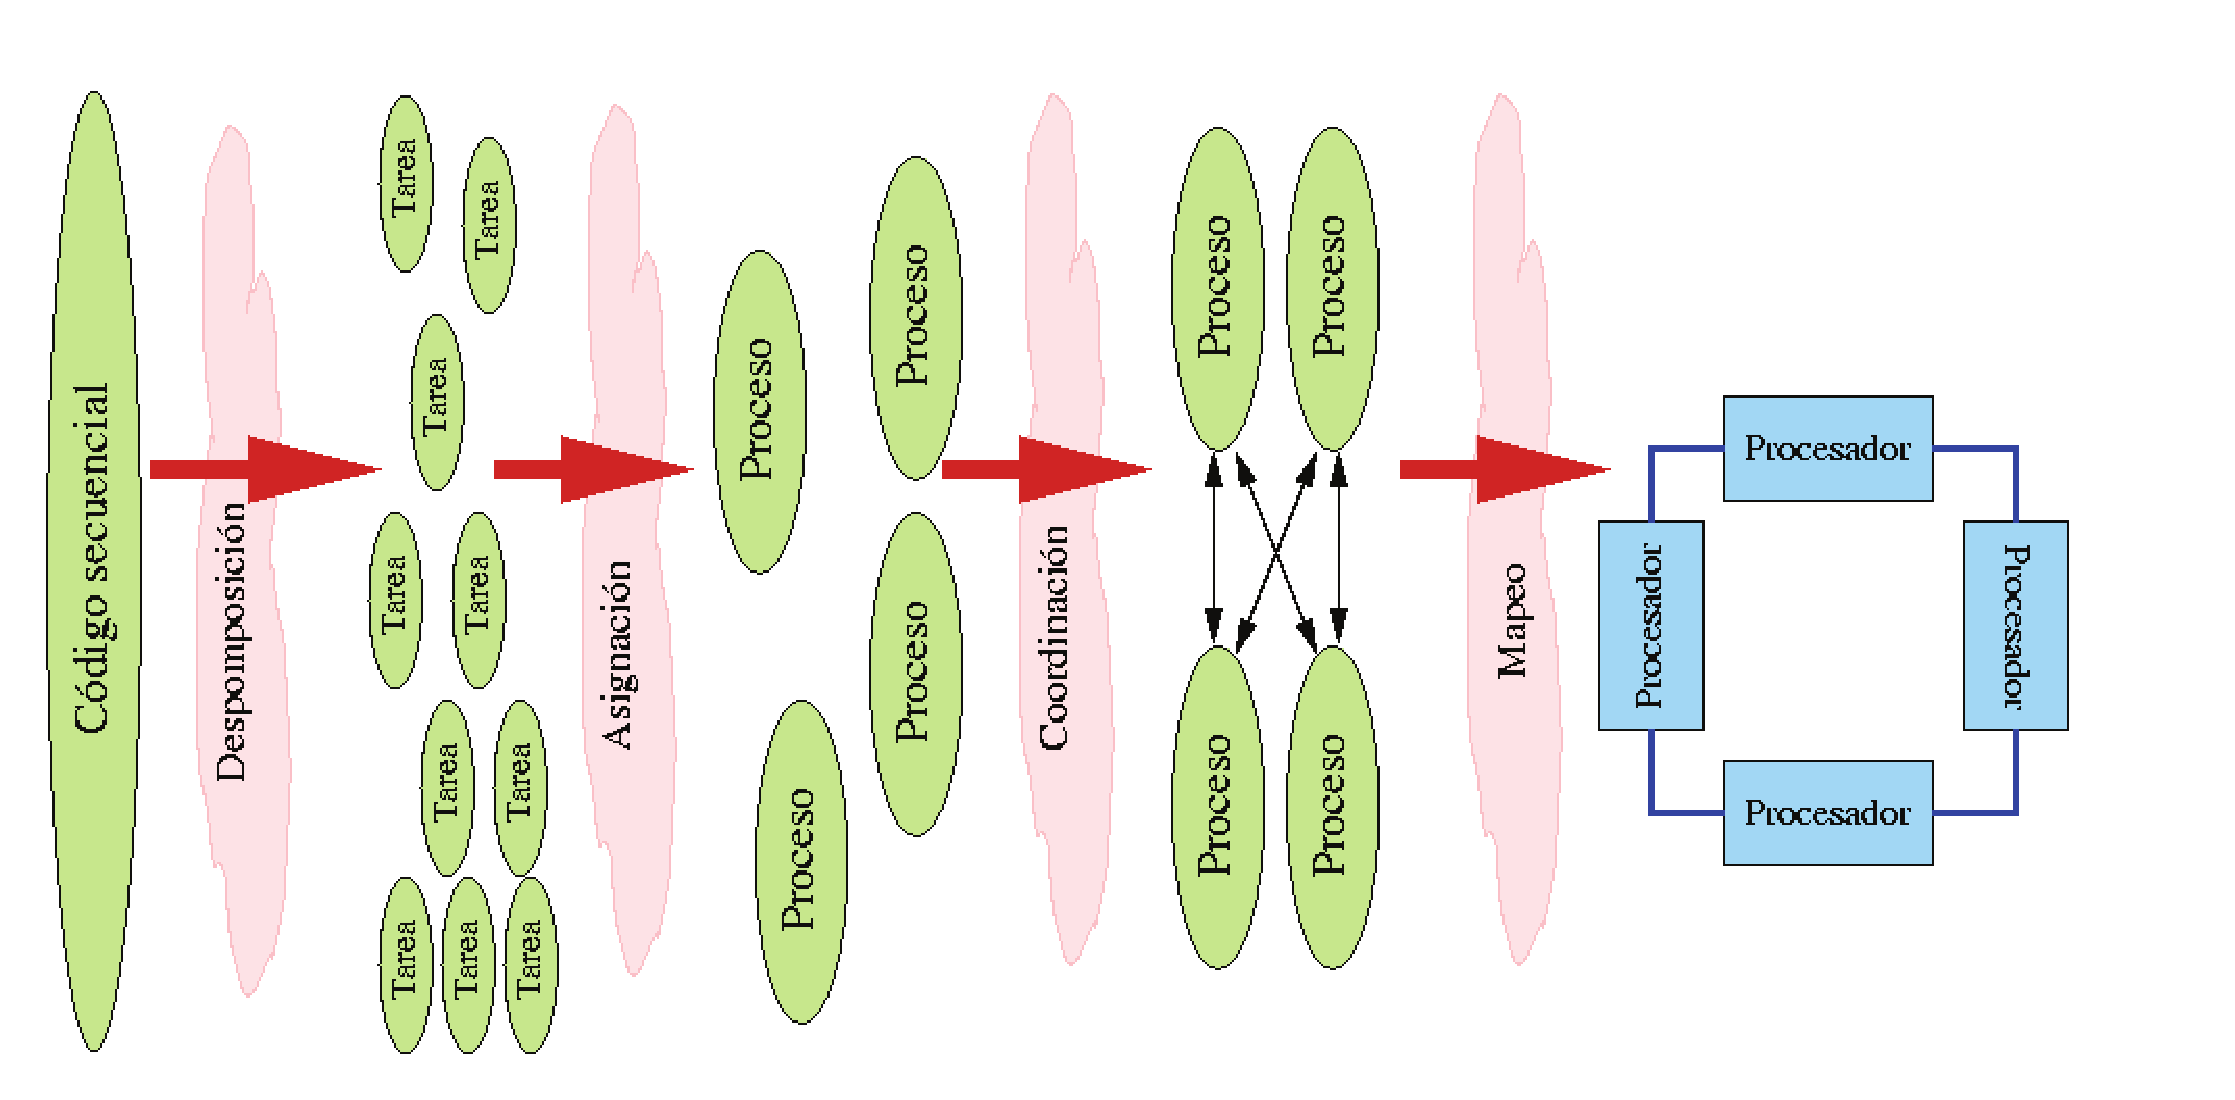
\includegraphics[width=15cm]{figuras/figura01.eps}}
\caption{Esta é a figura de tal e cal.}
\label{enlace1}
\end{figure}

\begin{table}
\begin{center}
\begin{tabular}{|l||r|c|} \hline
Izquierda & Derecha & Centrado  \\ \hline\hline
ll & r & cccc \\ \hline
llll & rrr & c \\ \hline
\end{tabular}
\caption{Esta é a táboa de tal e cal.}
\label{enlace2}
\end{center}
\end{table}

\section{Exemplos de referencias á bibliografía}
Este é un exemplo de referencia a un documento descargado da web \cite{cuda}. E este é un exemplo de referencia a unha páxina da wikipedia \cite{cdma}. Agora un libro \cite{gonzalez} e agora unha referencia a un artigo dunha revista \cite{patricia}. Tamén se poden pór varias referencias á vez \cite{cuda,gonzalez}.

\section{Exemplos de enumeracións}

Con puntos:

\begin{itemize}
\item Un.
\item Dous.
\item Tres.
\end{itemize}

Con números:

\begin{enumerate}
\item Catro.
\item Cinco.
\item Seis.
\end{enumerate}

Exemplo de texto verbatim:

\begin{verbatim}
O texto        verbatim 
     se visualiza tal
            como se escribe
\end{verbatim}

Exemplo de código C:

\lstset{language=C}

\begin{lstlisting}
#include <math.h>
main()
{  int i, j, a[10];
   for(i=0;i<=10;i++) a[i]=i; // comentario 1
   if(a[1]==0) j=1; /* comentario 2 */
   else j=2;
}
\end{lstlisting}

Exemplo de código Java:

\lstset{language=java}

\begin{lstlisting}
class HelloWorldApp {
    public static void main(String[] args) {
        System.out.println("Hello World!"); // Display the string.
    }
}
\end{lstlisting}



% Engadir os capitulos que fagan falta
%
%\cleardoublepage
%\chapter{Conclusións e posibles ampliacións}

Conclusións e posibles ampliacións


% Aquí empezan os apéndices
%\appendix
%\cleardoublepage
%\chapter{Manuais técnicos}

Manuais técnicos: en función do tipo de Traballo e metodoloxía empregada, o contido poderase dividir en varios documentos. En todo caso, neles incluirase toda a información precisa para aquelas persoas que se vaian a encargar do desenvolvemento e/ou modificación do Sistema (por exemplo código fonte, recursos necesarios, operacións necesarias para modificacións e probas, posibles problemas, etc.). O código fonte poderase entregar en soporte informático en formatos PDF ou postscript.

%\cleardoublepage
%\chapter{Manual de instalación}

El proyecto ha sido desarrollado en Linux por lo que la instalación deberá hacerse a través de ese sistema operativo. 


Se deben seguir los siguientes pasos:

\begin{enumerate}
\item Se abre la terminal.
\item Sitúate sobre el directorio del proyecto \texttt{em_web} con el comando \texttt{cd}.
%\item \textbf{Instalación de la aplicación}
%\begin{enumerate}
%\item Se instala el gestor de paquetes NPM con el siguiente comando:
%%	\begin{listing}[style=consola, numbers=none]
%%	$ sudo apt-get install npm
%%	\end{listing}
%\item Se instalan todas las dependencias de la aplicación que se encuentran en la carpeta local \texttt{node_modules}, y que están listadas como dependencias en el archivo \texttt{package.json}:
%
%\end{enumerate}
%\item Instalación del gestor de bases de datos
%\begin{enumerate}
%\item Se instala MongoDB con:
%
%\item Para correr MongoDB se utiliza:
%
%\item Se crea la base de datos de Emozio con el comando que aparece a continuación. Una vez creada la base de datos, se puede acceder a ella con el mismo comando.
%
%\item Se cargan los datos en la base de datos ejecutando:
%
%\end{enumerate}
\end{enumerate}

%\cleardoublepage
%\chapter{Licenza}
Se se quere pór unha licenza (GNU GPL, Creative Commons, etc), o texto da licenza vai aquí.


%\cleardoublepage
%\markboth{BIBLIOGRAFÍA}{BIBLIOGRAFÍA}
\addcontentsline{toc}{chapter}{Bibliografía}


\begin{thebibliography}{99}
%% EXEMPLO DE DOCUMENTO DESCARGADO DA WEB
%\bibitem{cuda} Nvidia CUDA programming guide. Versión 2.0, 2010. Dispoñible en {\it http://www.nvidia.com}.
%
%% EXEMPLO DE PÁXINA DA WIKIPEDIA
%\bibitem{cdma} Acceso múltiple por división de código. Artigo da wikipedia ({\it http://es.wikipedia.org}). Consultado o 2 de xaneiro do 2010.
%
%% EXEMEPLO DE LIBRO
%\bibitem{gonzalez} R.C. Gonzalez e R.E. Woods, {\it Digital image processing}, 3ª edición, Prentice Hall, New York, 2007.
%
%% EXEMPLO DE ARTIGO DE REVISTA
%\bibitem{patricia} P. González, J.C. Cartex e T.F. Pelas, ``Parallel computation of wavelet transforms using the lifting scheme'', {\it Journal of Supercomputing}, vol. 18, no. 4, pp. 141-152, junio 2001.

%%%%%%%%%%%%%%%%%%%%%%%%%%%%%%%%%%%%%%%%%%%%%%%%%%
%REALES
%%%%%%%%%%%%%%%%%%%%%%%%%%%%%%%%%%%%%%%%%%%%%%%%%%
% PMBOK
\bibitem{pmbok} PMBOK blablabla

% Pressman: Ingeniería del software. Un enfoque práctico
\bibitem{pressman} Pressman blablabla

\bibitem{sommerville} Sommerville blabla

\bibitem{github} GitHub  blaabla

\bibitem{mongodb_traspas} The magical marvels of MongoDB ({\it http://courseware.codeschool.com/the-magical-marvels-of-mongodb/the-magical-marvels-of-mongodb-slides.pdf}). Consultado o 2 de xaneiro do 2010.

\bibitem{mongodb_blog_mean_stack} Blog MongoDB. The Stack MEAN ({\it https://www.mongodb.com/blog/post/the-mean-stack-mongodb-expressjs-angularjs-and}). Consultado o 2 de xaneiro do 2010.

\bibitem{mongodb} MongoDB ({\it https://www.mongodb.com/es})

\bibitem{expressjs} ExpressJS ({\it http://expressjs.com/es/})

\bibitem{angularjs_arch} AngularJS Guide Architecture ({\it https://angular.io/guide/architecture})

\bibitem{angularjs_docs} AngularJS Docs ({\it https://angular.io/docs})

\bibitem{nodejs_about} NodeJS About ({\it https://nodejs.org/es/about/})

\bibitem{bootstrap_get} GetBootstrap ({\it http://getbootstrap.com/2.3.2/})

\bibitem{semanticui_github} Semantic UI GitHub ({\it https://github.com/Semantic-Org/Semantic-UI}) 



\end{thebibliography}



%%%%%%%%%%%%%%%%%%%%%%%%%%%%%%%%%%%%%%%%%%%%%%%%%%%%%%%%%%%%%%%%%%%%%%%%%%

\newpage
%\nocite{*}
%\bibliographystyle{unsrt}
\bibliographystyle{plain}
\bibliography{capitulos/biblio}

\end{document}
